\chapter{\textsc{Solas}, a 3-D Laser Ray-Trace and Cross-Beam Energy Transfer Model}%
\label{chap:SOLAS}

This chapter describes the \textsc{Solas} code, a 3-D laser ray-tracing module implemented in the \ac{Rad-MHD} code \textsc{Chimera}.
The chapter begins with a discussion of why ray-tracing is frequently used to model `long-pulse' lasers for \ac{HEDP} experiments and why the standard framework is inadequate to model \ac{LPIs}.
It then goes on to describe the ray-trajectory solver, electric-field reconstruction and \ac{CBET} components of the model in detail, including discussion of the validity of the model components.
The numerical methods are also presented alongside an extensive set of validation problems to verify the implementation.

\newpage

%###############################################################################################################################
%###############################################################################################################################
%###############################################################################################################################
\section{Ray-Tracing for Hydrodynamic Simulations of Fusion Plasmas}%
\label{sec:SOLAS_raytracing_for_ICF}

Nanosecond length (`long-pulse') lasers are often used as an external energy source in the field of \ac{HEDP}, for example in laboratory-astrophysics experiments~\cite{tzeferacos_laboratory_2018,fiuza_electron_2020,meinecke_strong_2022}, equation of state studies~\cite{kritcher_measurement_2020,smith_ramp_2014} or \ac{ICF} implosions~\cite{zylstra_burning_2022,slutz_highgain_2012,williams_demonstration_2024}.
Experimental design and analysis for these experiments must often be supported with fluid \ac{Rad-MHD} simulations.
The laser must therefore be described in these codes by a theoretical framework that is both valid and computationally tractable.
The physical processes by which lasers interact with plasma are a result of microscopic couplings between the laser field and particles or plasma waves.
The detailed microphysics of these interactions are often studied using \ac{PiC} codes~\cite{nguyen_crossbeam_2021} or wave-based solvers~\cite{myatt_wavebased_2017}, typically for scales and durations of tens of micrometres and hundreds of picoseconds.
Coupling these tools directly to multidimensional \ac{Rad-Hydro} simulations, which are often used for millimetre and nanosecond scales, is usually computationally intractable.

The \ac{GO} assumptions are often applicable for \ac{HEDP} laser-plasma interactions and therefore ray-tracing offers a computationally tractable approach to modelling lasers in these experiments\footnote{Validity is discussed in detail for \ac{ICF} plasmas in Sec.~\ref{sec:Theory_GO_appliciability}}.
By assuming static \ac{Rad-Hydro} profiles (which is normally valid for the propagation time of light through the computational domain) a laser beam can be discretized into a bundle of rays.
The ray equations can then be integrated along their path to solve for the trajectory of the light, assuming that refraction dominates over diffraction.
A discrete amount of power can also be given to each ray.
If there is a suitable model for the power-absorption rate, this can also be integrated along the ray to provide an energy source for the plasma.
In many laser-driven \ac{HEDP} experiments, frequency-doubled or -tripled lasers and long scale-length plasmas mean that \ac{Inv-Brem} is the dominant deposition process~\cite{schmitt_importance_2023,schmitt_importance_2023a}.
There are well established models for \ac{Inv-Brem} that are suitable for implementation in ray-tracing codes, because they only require knowledge of the local plasma conditions, which are easily accessible via interpolation from the \ac{Rad-Hydro} grid to ray locations~\cite{huba_nrl_2013,johnston_correct_1973}.
The combination of the ray equations and \ac{Inv-Brem} deposition is therefore the basis for the vast majority of laser-modules coupled to \ac{Rad-Hydro} codes.

In laser-driven \ac{ICF} experiments however, another class of interaction, \ac{LPIs}, are vitally important to the energetics of the implosion.
For example, \ac{CBET} leads to a zeroth-order correction to the energy deposited in direct-drive experiments at the \textsc{Omega} laser facility, reducing coupled power late in the implosion to $\sim 50\%$~\cite{colaitis_inverse_2021}.
\ac{LPIs} cannot be included in the simple framework described above for two reasons.
Firstly, they are non-linear\footnote{Non-linear in this context means that the interaction involves multiple light and plasma waves.} and secondly, reduced theoretical models of the interaction rely on knowledge of the electric field or intensity of the light~\cite{randall_theory_1981}.
Implementation in a ray-tracing code therefore necessitates a method by which the separate light waves can `talk' to each other.
For example, the \ac{CBET} code described in this chapter stores information for separate components of laser beams on a common grid, which can then interact via the `pump-depletion iterations', described in Sec.~\ref{sec:pump_dep_iters}.
Additionally, calculating the electric field or intensity is problematic because this is not an attribute which can be obtained from a \ac{GO} ray.
Heuristically, rays have an associated power, so an area is required to obtain an intensity.
The evolution of a portion of the beam front's area is governed by a first order expansion of the Helmholtz equation, rather than the zeroth order expansion, which is most commonly used in ray-tracing packages for \ac{Rad-Hydro} codes~\cite{colaitis_modeling_2014}.
The first order expansion introduces an equation for the ray amplitude, which can be solved in a variety of ways and used to obtain the electric field of the light.
Sec.~\ref{sec:SOLAS_field_reconstruc} describes the approach taken to solving for the amplitude of the rays in \textsc{Solas}, which is to track the area of a triangle\footnote{For a 2-D ray-trace, a co-planar, pair of rays is used rather than a triangle.} of rays around a standard \ac{GO} ray.

For direct-drive \ac{ICF} simulations, it is also desirable to have a 3-D ray-trace, where rays travel and refract in three dimensions.
In some computational direct-drive studies, particularly in 1-D \ac{Rad-Hydro} simulations, simplified laser models are employed in which rays travel radially toward the target~\cite{paddock_onedimensional_2021}.
This simplification can lead to significant deviations from reality, as it neglects any refractive losses, which become increasingly significant late in the implosion as the target converges.
Assuming that rays travel radially inward, also leads to deposition occurring closer to the critical surface compared to a true 3-D ray-trace, resulting in an overestimation of the drive.
The growth of \ac{LPIs} also depends on vector summations of light and plasma wavevectors, so a 3-D ray-trace is necessary when modelling these effects.
Predictive direct-drive simulations therefore necessitate a fully 3-D ray-trace, even when coupled to just 1-D hydrodynamics.


%###############################################################################################################################
%###############################################################################################################################
%###############################################################################################################################
\section{Existing Cross-Beam Energy Transfer Models}

There is a variety of existing computational tools used to model \ac{CBET} for \ac{ICF} conditions.
These include codes that are used to study the interaction from first principles, reduced models to investigate the effect of \ac{CBET} when coupled to hydrodynamics and validation tools to test the implementation of these reduced models.
A non-exhaustive list of existing codes is listed below, provided as context for the work presented later in this chapter.

%################################################################################
%################################################################################
\subsection{Ray-Based Models}

The most common tool to study the coupling of \ac{CBET} effects into hydrodynamics are reduced ray-based models, which use the linear gain theory of \ac{SBS}, described in more detail in Sec.~\ref{sec:SOLAS_cbet_model}.
A variety of different codes used to study this.
The main difference between the models is the way that the electric field or intensity of the laser light is obtained.

\paragraph*{\ac{IRT}} This is an approach implemented in the \textsc{Ifriit} code, that creates a mapping between points on an initial beam front and arbitrary locations within the plasma~\cite{colaitis_real_2019,colaitis_adaptive_2019}.
This is in contrast to \ac{FRT}, used in the other ray-based approaches listed below, where discrete points on the beam front are integrated forward to discrete points within the plasma.
\ac{IRT} is an efficient approach for convex, approximately spherically symmetric plasma profiles, but cannot deal well with beams that have multiple caustics\footnote{Caustics are defined and discussed in detail in Sec.~\ref{sec:SOLAS_ray_amplitude}.}, where the \ac{FRT} approach is better suited.
\textsc{Ifriit} has been coupled to the 3-D \ac{Rad-Hydro} code, \textsc{Aster} from \ac{LLE}, and prior to the development of \textsc{Chimera}-\textsc{Solas}, \textsc{Aster}-\textsc{Ifriit} was the only code combination capable of conducting 3-D direct-drive simulations with in-line \ac{CBET}~\cite{colaitis_inverse_2021}.

\begin{figure}[t!]
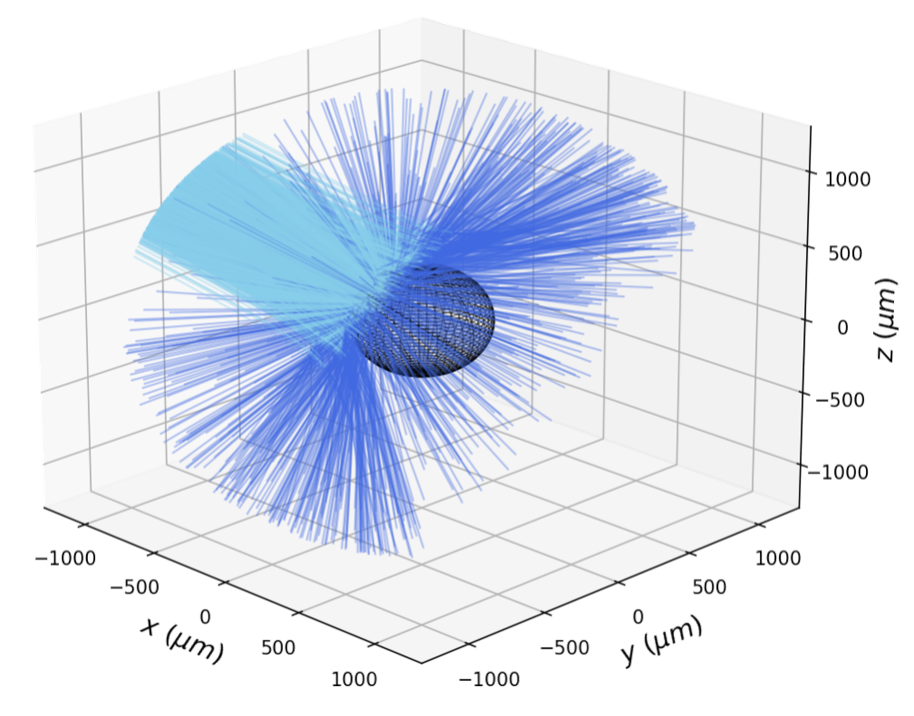
\includegraphics[width=10cm]{Numerics/Images/Reflected_Rays.png}
\centering
\caption{3-D ray trajectories through a spherically symmetric, \textsc{Omega} direct-drive scale density profile.
The incident rays are plotted in cyan and the reflected rays, which spread out over a large solid angle, are plotted in dark blue.
The critical density is represented by the black mesh.}%
\label{fig:reflectedrays}
\end{figure}

\paragraph*{Ray Statistics Approach} The \textsc{Lasnex}~\cite{strozzi_interplay_2017}, \textsc{Troll}~\cite{liberatore_first_2023} and \textsc{Draco} codes~\cite{marozas_wavelengthdetuning_2018}, developed at \ac{LLNL}, \ac{CEA} and \ac{LLE} respectively, implement field-reconstruction methods, which depend heavily on having many rays per computational cell.
\textsc{Lasnex} and \textsc{Troll}, used mainly for indirect-drive hohlraum simulations, obtain the intensity of light by first propagating rays through the mesh and obtaining the deposited power in each grid cell.
The intensity is then obtained from the power in each cell using electromagnetic energy conservation.
Obtaining the intensity from deposition means that the field cannot be reconstructed in vacuum regions where no deposition occurs.

\textsc{Draco} uses a similar approach, but the intensity is estimated by multiplying the ray power by the path length in a cell and dividing by the cell volume, which gives a dimensional estimate for the intensity.
Both of these approaches require many rays-per-cell to accurately obtain the intensity, $\mathcal{O}(100)$~\cite{debayle_unified_2019}.
For direct-drive simulations this is extremely computationally expensive, because backscatter \ac{CBET} dominates over sidescatter.
Therefore, the reflected field of each beam must be resolved, and each beam spreads out over a large solid angle after reflecting off a convex density profile, as is demonstrated in Fig.~\ref{fig:reflectedrays}.
This means that orders of magnitude more rays are required, compared to approaches which can accurately obtain the field from a single ray per cell.

Another drawback of both of these approaches is that caustics of beams (regions where the amplitude of rays diverge) are not identifiable, and therefore fields cannot be capped to physically accurate, diffraction-limited values.
If a significant amount of \ac{CBET} occurs at caustics, such as in direct-drive \ac{ICF}, then erroneous global multipliers to \ac{CBET} gains must be applied which are effectively free parameters that must be tuned to obtain a pre-known reduction in absorbed energy.
It is therefore difficult to trust this approach for predictive, pre-shot direct-drive simulations.

\paragraph*{\ac{PCGO}} In this approach, each ray has an associated Gaussian intensity profile, the width of which is integrated along the ray trajectory~\cite{colaitis_modeling_2014,colaitis_crossed_2016}.
A single ray can be used per cell because each ray therefore has an intensity which is interpolated to the mesh.
However, the reconstructed field near caustics is not accurate and the width evolution is only valid for a short propagation distance.
This approach was coupled to the \textsc{Chic} 2-D \ac{Rad-Hydro} code, but the approach is difficult to extend to 3-D as the implementation relied on interacting only rays whose centroids crossed, which does not occur in 3-D for non-coplanar rays~\cite{colaitis_modeling_2015}.

\paragraph*{Neighbouring Rays} The \textsc{BeamCrosser} code obtains an area for each ray by co-tracing a triangle of neighbouring rays around it that can be converted into a ray amplitude and therefore electric field from electromagnetic energy conservation~\cite{edgell_mitigation_2017}.
Integrating the amplitude along the ray trajectory means that the caustics can be identified and therefore fields in those regions capped to diffraction limited values~\cite{follett_raybased_2018}.
Each ray also has an individual field value, and it is therefore less dependent on ray-per-cell statistics than geometric models, such as that used in the \textsc{Draco} code described above~\cite{follett_validation_2022}.
Sec.~\ref{sec:SOLAS_field_reconstruc} describes the implementation of this approach into the \textsc{Chimera} 3-D \ac{Rad-MHD} code.
A similar approach, simplified by assuming uniform illumination of a direct-drive target, has been implemented into the 1-D \textsc{Lilac} \ac{Rad-Hydro} code~\cite{igumenshchev_crossedbeam_2010, igumenshchev_crossedbeam_2012}.
It had previously however, not been coupled to a multidimensional \ac{Rad-Hydro} code.


%################################################################################
%################################################################################
\subsection{Wave Solvers}

Solving Maxwell's equations in a plasma background is a useful tool for the study of \ac{LPIs}.
The main code used in the \ac{ICF} community that uses this approach is \textsc{Lpse}, which propagates light waves through a prescribed, spatially varying density, temperature and velocity profile in 1-D$\rightarrow$3-D~\cite{myatt_wavebased_2017,myatt_lpse_2019}.
It then solves the nonlinear coupling of electromagnetic waves by allowing first order plasma perturbations (obtained from the ponderomotive beat pattern between light waves), which then feed back into the wave propagation.
The perturbative approach limits \textsc{Lpse} to linear problems and the temporal and spatial resolution required to resolve the beat frequency mean that coupling to multidimensional \ac{Rad-Hydro} simulations is not feasible.
However, it is an extremely useful tool to validate implementation of \ac{CBET} models, especially for laser caustics where diffraction is important, such as the test case presented in Sec.~\ref{sec:SOLAS_CBET_caustic_test}.
It can also been used for many other important studies, such as the mitigation of \ac{LPIs} via laser bandwidth and the effect of beam smoothing techniques on the growth rate of \ac{LPIs}~\cite{follett_thresholds_2021}.

%################################################################################
%################################################################################
\subsection{Particle in Cell Codes}

Both ray-based codes and \textsc{Lpse} are ill-suited to the study of \ac{LPIs} in the non-linear regime, where the laser intensity becomes sufficiently large that the ponderomotive imprint on the plasma can no longer be treated perturbatively.
Understanding the growth and saturation of \ac{LPIs} in this regime is particularly important for \ac{ICF} schemes with high peak intensities, such as during the ignitor spike in shock ignition pulses~\cite{perkins_shock_2009}.
Often kinetic effects such as ion-trapping become important in non-linear saturation, where ions are trapped and then accelerated in the \ac{CBET} induced \ac{IAW}, leading to changes in the \ac{IAW} phase velocity and therefore a loss of resonance~\cite{nguyen_crossbeam_2021}.
\ac{PiC} codes operate by using a finite number of macro-particles to represent the distribution function of the plasma, coupled to an electromagnetic solver, discretised on a mesh.
They are therefore well suited to model this kinetic saturation, albeit over short timescales and in simulations that are not truly representative of direct-drive conditions, due to computational expense~\cite{seaton_crossbeam_2022a}.
Kinetic modelling of \ac{CBET} has demonstrated that the growth of \ac{LPIs} can be a much more complex, time-dependent problem than is assumed by the linear-models used in ray-based codes, leading to larger net energy transfers~\cite{seaton_crossbeam_2022}.

%###############################################################################################################################
%###############################################################################################################################
%###############################################################################################################################
\section{\textsc{Solas} 3-D Laser Ray-Trace}%
\label{sec:SOLAS_raytrace}

This section describes how the ray equations, derived from the Helmholtz equation in Sec.~\ref{sec:theory_ray_equations} are solved in the \textsc{Solas} module for the \textsc{Chimera} \ac{Rad-MHD} code.
Details of the mesh used for spherical simulations, load balancing options as well as validation problems are provided.

A short summary of the computational derived-types is presented here, to aid understanding of the following sections.
In \textsc{Solas}, a domain balanced mesh is created from the hydrodynamic grid in \textsc{Chimera}.
The mesh is made up of \textit{laser-cells}, which hold information about the geometry, hydrodynamic-quantities, laser-quantities\footnote{Laser quantities include, for example, \ac{Inv-Brem} deposition and electric field strength.} and neighbouring cells on the \textsc{Solas} grid.
\textit{Beam} objects are created which hold user-defined geometric information about the beam-port and pointing location and also store a list of rays from the beam.
Each ray is defined by a position $(\mathbf{x})$, wavevector $(\mathbf{k})$, phase $(\varphi)$\footnote{Note that the phase $\varphi$ has units of space. It can be converted to the dimensionless phase, $\psi=k_0\varphi$, where $k_0$ is the vacuum wavenumber.}, angular frequency $(\omega)$ and power ($P$).
If field reconstruction is performed, then each ray also stores up to three additional \textit{neighbour-rays}, from which the electric field of the ray can be reconstructed, as described in Sec.~\ref{sec:SOLAS_field_reconstruc}.

%################################################################################
%################################################################################
\subsection{Outline of \textsc{Solas}-\textsc{Chimera} Interfacing}

\begin{figure}[t!]
    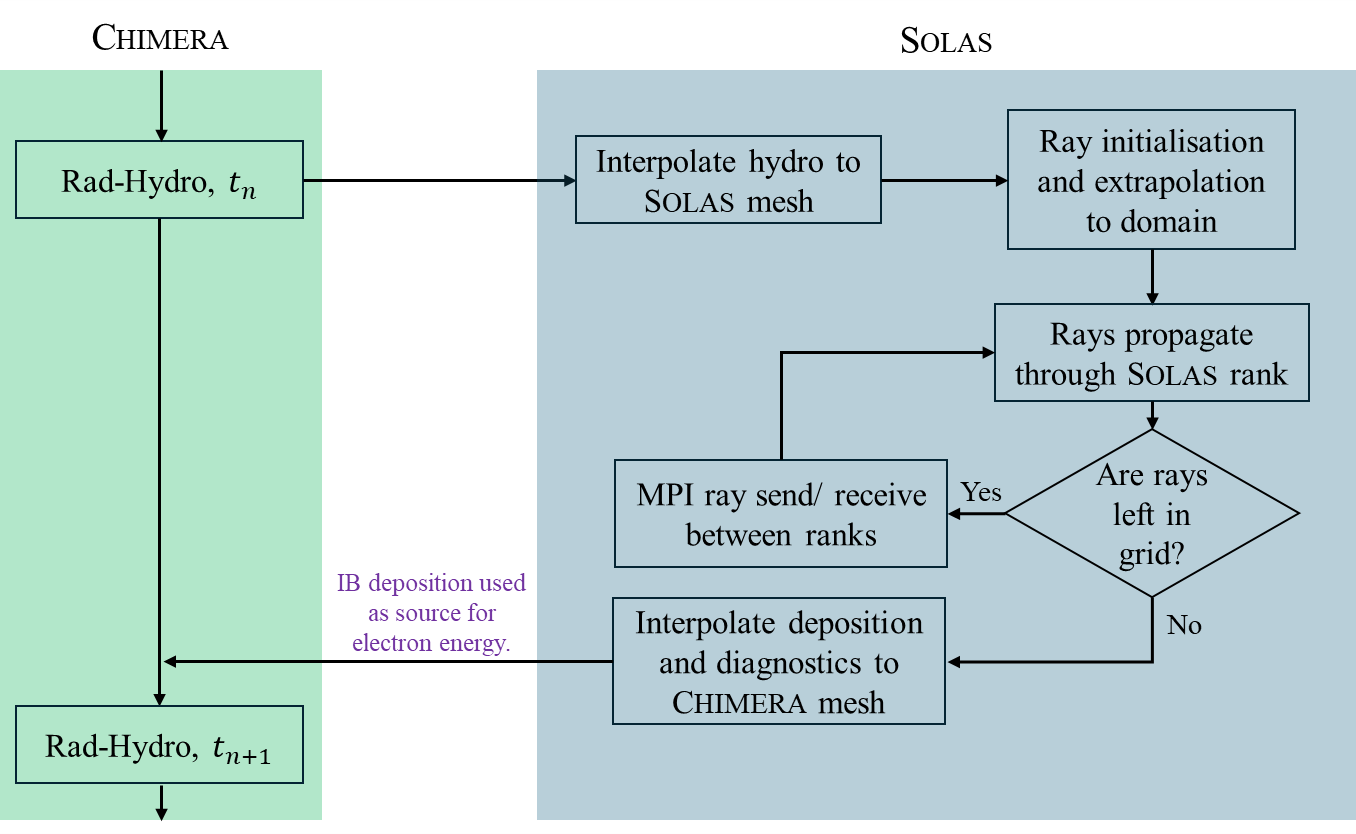
\includegraphics[width=0.9\linewidth]{Numerics/Images/raytrace_flowchart.png}
    \centering
    \caption{A flowchart illustrating the basic interfacing between \textsc{Chimera} and \textsc{Solas}.
    The interpolation steps refer simultaneously to the re-domain balancing and cell combination procedures described in Sec.~\ref{sec:SOLAS_mesh}.}%
    \label{fig:raytrace_flowchart}
\end{figure}

A simple flowchart for the basic \textsc{Solas} operational loop and the interfacing with \textsc{Chimera} is shown in Fig.~\ref{fig:raytrace_flowchart}.
At the start of a \ac{Rad-Hydro} timestep, $t_n$, the hydrodynamic variables (stored on the Eulerian \textsc{Chimera} grid), which are necessary to compute ray trajectories and \ac{CBET} gains, are interpolated to the \textsc{Solas} mesh.
Rays are then initialised on the beam port locations and extrapolated to the computational domain, before being traced through the grid.
\textsc{Solas} uses an \ac{MPI} domain balanced approach to parallelisation, the reasons for which are discussed in more detail in Sec.~\ref{sec:SOLAS_mesh}, therefore rays are traced up to the internal borders of the \ac{MPI} rank subdomain.
Rays are then passed between ranks and moved through their new subdomain until they exit the entire simulation domain.
As rays move through the domain, they lose energy via \ac{Inv-Brem}, contributing to a running deposition total in each grid cell.
When all rays have exited the domain, the \textsc{Solas} quantities, such as deposited energy which have been built up from the ray-trace, are then interpolated onto the \textsc{Chimera} grid, where the \ac{Inv-Brem} deposition is used as a source term for the electron energy in the subsequent \ac{Rad-Hydro} step, $t_{n+1}$.
The interpolation, initialisation and propagation steps are outlined in sections~\ref{sec:SOLAS_mesh},~\ref{sec:SOLAS_ray_init},~\ref{sec:SOLAS_ray_propagation} respectively.


%################################################################################
%################################################################################
\subsection{\textsc{Solas} Mesh Structure}%
\label{sec:SOLAS_mesh}

For direct-drive \ac{ICF} simulations, which model the laser using ray-tracing (especially those which include \ac{CBET}), the choice of an appropriate computational mesh on which to conduct the laser ray-trace is crucial to obtaining an accurate and noise-free energy deposition.
A well-chosen grid can also significantly reduce the run-time and memory requirements of the calculation.
The mesh used for hydrodynamic simulations of these experiments is often not well suited for ray-tracing calculations.
For example, hydrodynamic grids often have excessive resolution in the corona to resolve the gradients in the laser quantities, which greatly increases the expense of tracing rays through the mesh, without significantly enhancing the accuracy of the solution.
This section describes the approach taken in the \textsc{Solas} code to create a grid structure that accurately resolves laser energy deposition, both with and without \ac{CBET}, in a memory-efficient manner.

%##################################################
\subsubsection{Re-Domain Balance for Radial Geometries}

\begin{figure}[t!]
    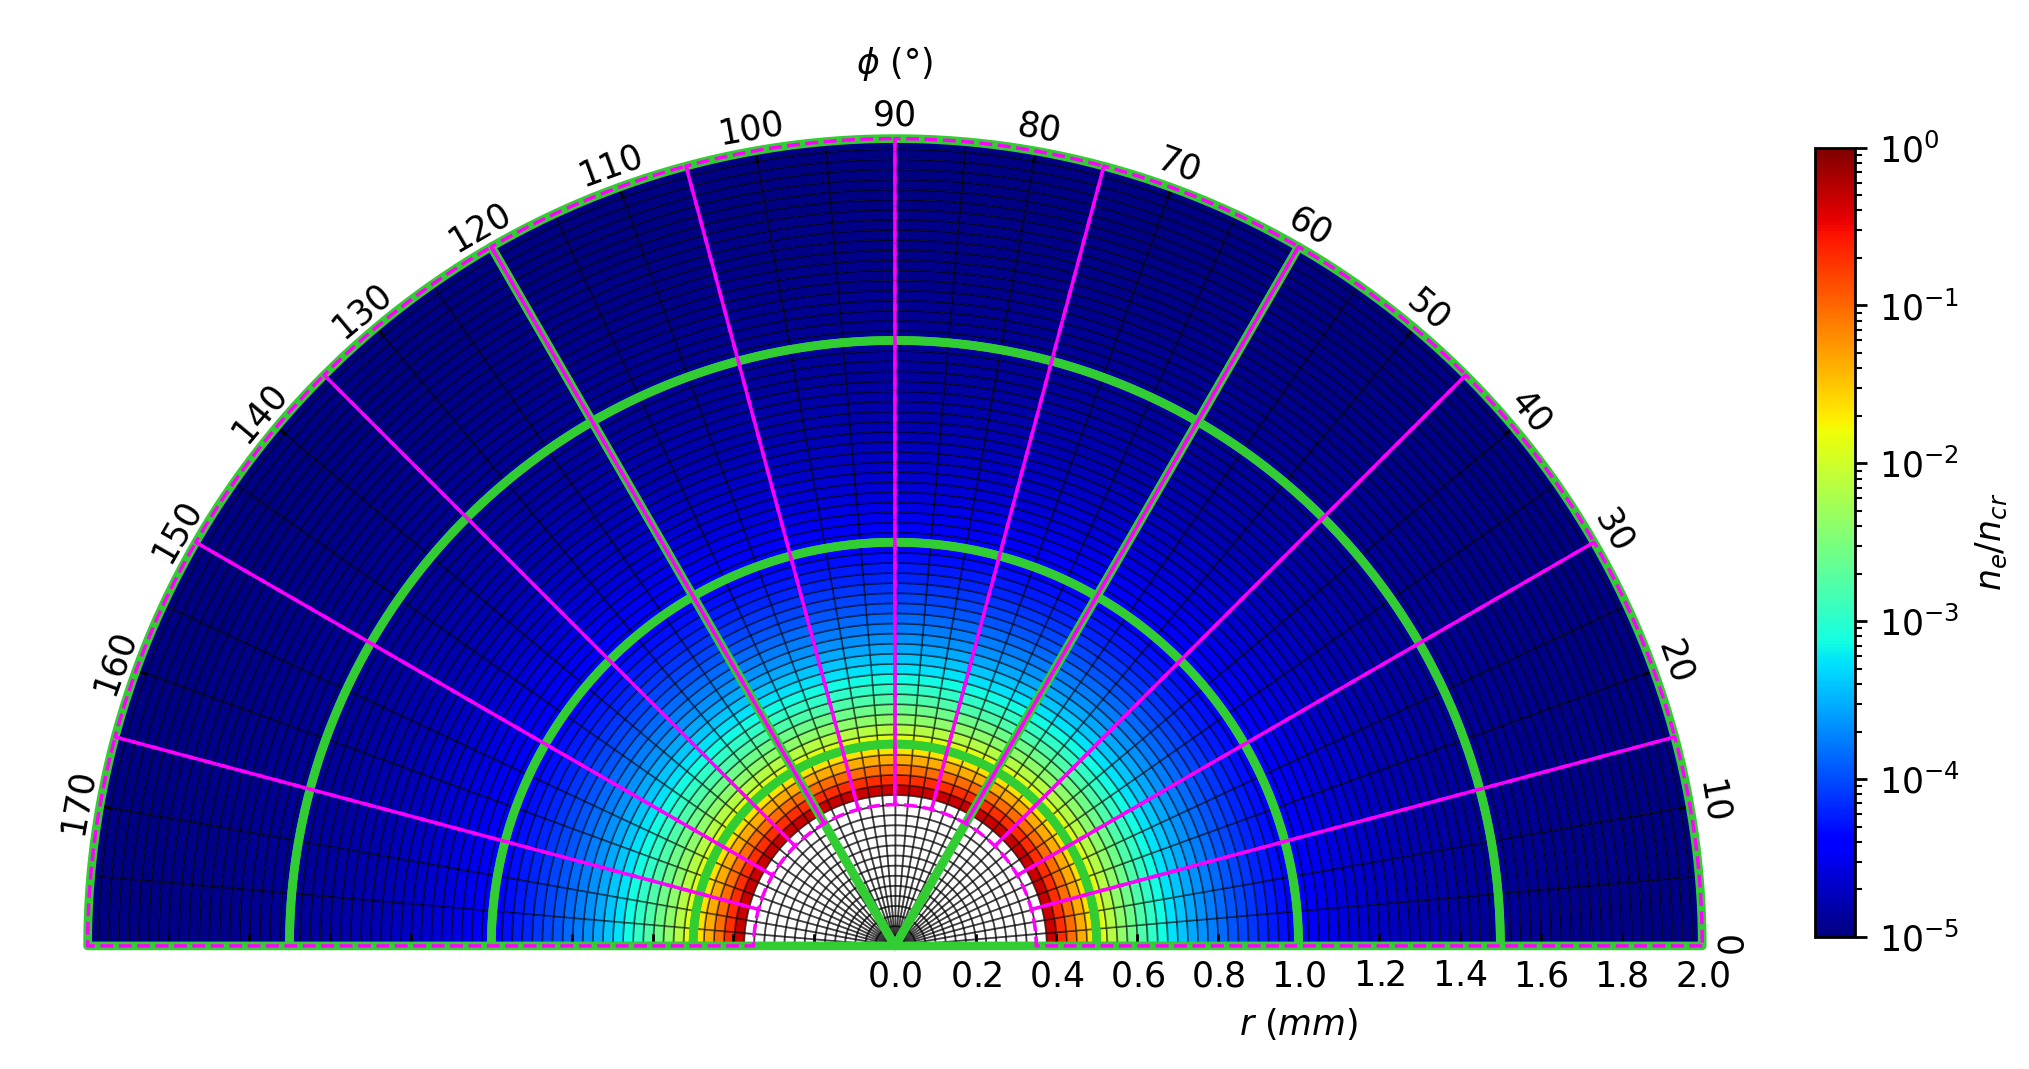
\includegraphics[width=\linewidth]{Numerics/Images/SOLAS_CHIMERA_domain.png}
    \centering
    \caption{An illustrative diagram demonstrating the MPI re-domain balanced grid employed by \textsc{Solas} compared to the \textsc{Chimera} domain balanced grid for a cylindrical geometry.}%
    \label{fig:SOLAS_CHIMERA_domain}
\end{figure}

\ac{Rad-MHD} codes including \textsc{Chimera}, often employ a domain balanced approach to parallelisation, where each computational rank solves a portion of the entire spatial domain, for each discrete timestep.
Additional `ghost-cells' are stored in the subdomains and used to calculate gradients on the boundaries between ranks, which are updated with inter-rank \ac{MPI} communications each timestep.
The hydrodynamic grid for \textsc{Chimera} is Eulerian, with options for Cartesian, cylindrical or spherical-polar grids.

The optimal domain balancing minimises the number of ghost cells at subdomain boundaries, which leads to cubic\footnote{Cubic in cell dimension, not necessarily in physical space for non-Cartesian geometries.} subdomains.
If computing a laser ray-trace through this domain for a typical direct-drive calculation however, initially rays travel approximately radially and therefore regularly encounter processor boundaries where they must be transferred between ranks.
A more optimal domain decomposition for the ray-trace minimises radial splitting to avoid excessive passing of rays.
For spherical and cylindrical simulations, \textsc{Solas} therefore takes the hydrodynamic variables on the \textsc{Chimera} grid and re-domain balances the grid for the ray-trace, such that the splitting does not occur in the radial coordinate.
An example of this re-domain balancing is shown in Fig.~\ref{fig:SOLAS_CHIMERA_domain} for an illustrative cylindrical mesh.
The \textsc{Chimera} domain decomposition divides the radial and azimuthal extent into four and three ranks respectively, whereas \textsc{Solas}' division is purely in the azimuthal direction.
For spherical and cylindrical direct-drive simulations where there is a defined, global minimum critical radius, \textsc{Solas}' mesh excludes the grid cells below this minimum radius beyond which the rays cannot reach in order to reduce the memory burden of the re-gridding.

An alternative approach to \ac{MPI}-based domain-decomposition parallelisation of the module is to use the \ac{OpenMP} package, for which ranks share memory across a computational node.
In this approach, the entire laser grid is stored once on the shared memory of the node and separate ranks trace rays through the entire domain without the need for transfers.
While this is a preferable approach for a standard ray-trace to the \ac{MPI} procedure described above, including a model for \ac{CBET} is more challenging.
This is because \ac{CBET} requires communication between beams and therefore large amounts of information must be stored on the grid, which can lead to large memory overheads.
Therefore, using multiple computing nodes is often a necessity for 3-D \ac{CBET} calculations for which \ac{OpenMP}-\ac{MPI} hybrid approaches are required.
This was deemed too significant an undertaking for the scope of the work presented in this thesis.

When a 3-D ray-trace is coupled to a lower dimensional hydrodynamics simulation (for example, a 1-D spherical direct-drive simulation) then a sparse 3-D mesh at a user-specified resolution is created for the ray-trace.
This 3-D mesh allows the re-domain balancing routine to be employed to load balance the simulation.
For \ac{CBET} simulations, it also allows the field, which is required to compute the power change of rays due to \ac{CBET}, to be stored as a function of angle when discretised on this sparse 3-D mesh.
Storing the field discretised in angle enables the interaction between beams around the sphere to be correctly computed.
After the ray-trace, if these extra dimensions have been added to the ray-trace grid, then the deposited power is integrated over the additional grid directions to obtain the source term on the hydrodynamic grid.

%##################################################
\subsubsection{Semi-Structured Eulerian Grid with Combined Cells}

\begin{figure}[t!]
    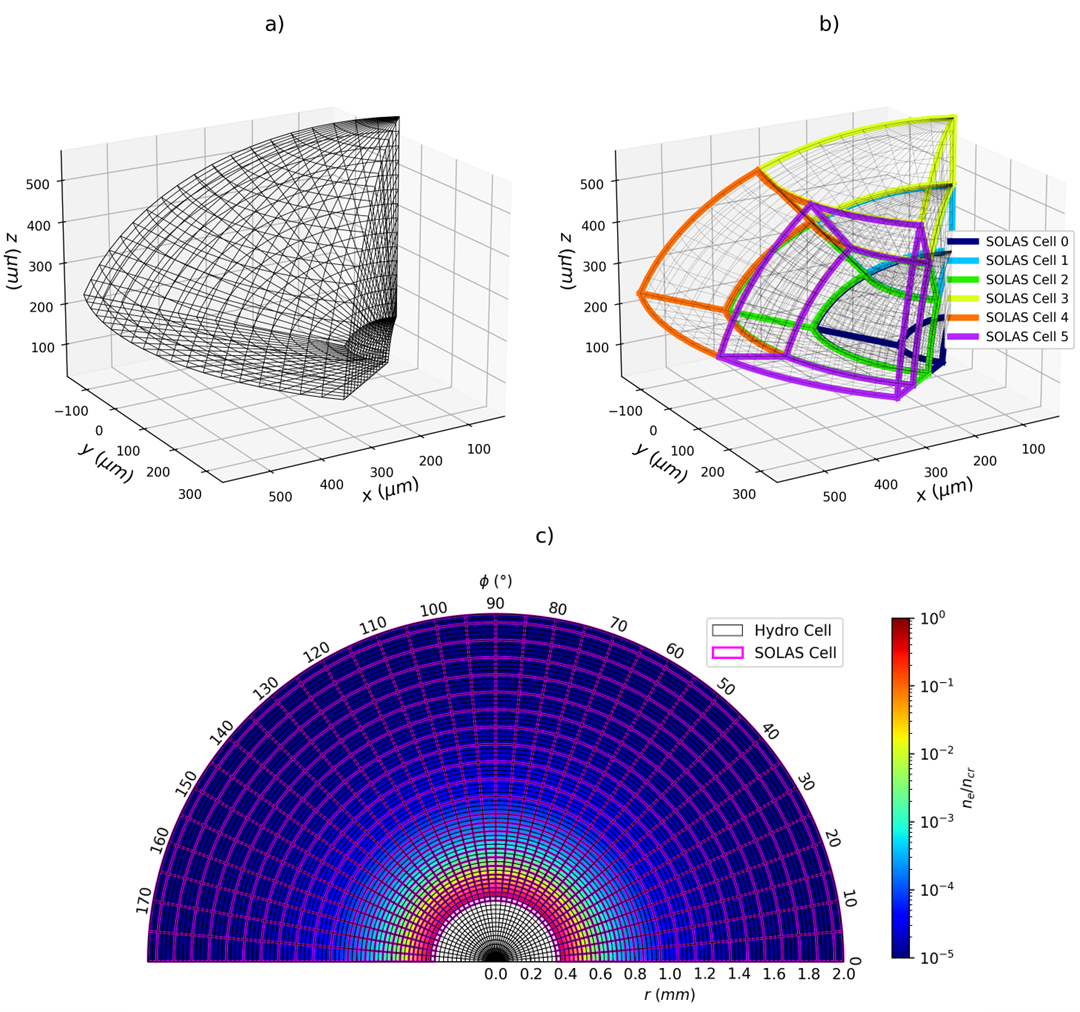
\includegraphics[width=\linewidth]{Numerics/Images/solas_cells_3imagescombined.png}
    \centering
    \caption{Illustrative diagrams demonstrating a) the spherical polar mesh used by \textsc{Chimera} for hydrodynamic calculations, b) the cell combination mechanism employed by \textsc{Solas} to obtain a roughly equal area grid for spherical simulations and c) the adaptive radial cell combination to reduce resolution in regions where \ac{CBET} and refraction are unimportant.}%
    \label{fig:SOLAS_combined_cells}
\end{figure}

Ideal \ac{ICF} implosions are spherically symmetric and departures from this symmetry are usually higher-order corrections.
Simulations of these experiments therefore typically employ a computational grid with spherical symmetry.
\textsc{Chimera} typically simulates direct-drive implosions with a spherical-polar Eulerian mesh, shown in Fig.~\ref{fig:SOLAS_combined_cells}.a.
This grid has the advantage of simplicity to take gradients across cells, however it has the disadvantage that cell edge lengths tend to zero as the radial coordinate, $r\rightarrow 0$ and the polar coordinate, $\theta\rightarrow 0,\pi$.
This limits the hydrodynamic timestep, because stable explicit timesteps are inversely proportional to edge lengths, increasing the cost of 3-D spherical simulations.
The issue is circumvented at late times in the implosion by remapping onto a Cartesian grid, which does not have vanishing edge lengths and face areas~\cite{chittenden_signatures_2016}.

Computing \ac{CBET} requires at least a single ray from each interacting beam to pass through each computational grid cell where the interaction should be important.
For spherical-polar meshes the vanishing cell volume therefore sets extreme minimum ray number limits for the calculation to fully resolve all the fields, particularly the reflected field in direct-drive simulations, which spreads out over $4\pi$ steradians, as is shown in Fig.~\ref{fig:reflectedrays}.
Hydrodynamic resolutions are often also excessive for ray-trace calculations to resolve the necessary refraction and energy exchange of the light.
Rays must also stop at each cell boundary in order to deposit the correct amount of energy into each grid cell and therefore the expense of the ray-trace is directly proportional to the number of grid cells that the rays see.

To circumvent these issues, cells can be combined around the spherical grid angles in order to make a semi-structured Eulerian grid, as is shown in Fig.~\ref{fig:SOLAS_combined_cells}.b.
Hydrodynamic grid cells are merged together on the \textsc{Solas} mesh in each grid direction until a pre-specified resolution, set by the user, is reached.
In Fig.~\ref{fig:SOLAS_combined_cells}.b, many cells are combined in each direction to clearly display the effect.
Typically, for spherical simulations however, the cells are not combined in the polar direction, $\theta$ and $n_{\varphi}$ cells are combined in the azimuthal direction until the azimuthal and polar resolutions match, explicitly $n_{\varphi}r\Delta\varphi\sin\theta \approx r \Delta\theta$ at a given radius, $r$.

Fig.~\ref{fig:SOLAS_combined_cells}.c demonstrates the capability of the meshing algorithm to adaptively combine cells in the radial direction based upon density gradients.
This allows large cells to exist in the coronal plasma where the light refracts minimally and deposits little energy, while the sharp turning point regions close to the critical surface can be well resolved.
To find the number of radial cells to combine at a given radius $n_r$, maximum gradient length scale from the combined hydrodynamic cells, $L_{n_e}=n_{crit}/|\nabla n_e|_{\max}$ is calculated.
The algorithm then finds the optimal number of cells to merge together such that the new cell resolution $n_r\Delta r \approx C_L L_{n_e}$, where $C_L$ is a user parameter\footnote{Default value set to $C_L=0.05$.} which can be reduced to limit cell combining.
A maximum cell size is also set to prevent excessively large cells in regions with small density gradients.

Note that many options for equal area computational grids exist which, unlike the semi-structured grid described here, are completely uncorrelated from the \ac{Rad-Hydro} mesh~\cite{cheong_eigensolutions_2015,malkin_new_2019}.
These have the advantage that the grid can be chosen purely based upon quantities important to the laser ray-trace.
However, the mesh described in this section has the advantage that interpolation to the hydrodynamic mesh is extremely straightforward as the \textsc{Solas} grid cells completely overlap the \textsc{Chimera} cells.
This also minimises artefacts from interpolation between the grids, which have the potential to introduce spurious high order modes to the deposition source term.

%################################################################################
%################################################################################
\subsection{Ray Initialisation}%
\label{sec:SOLAS_ray_init}

\begin{figure}[t!]
    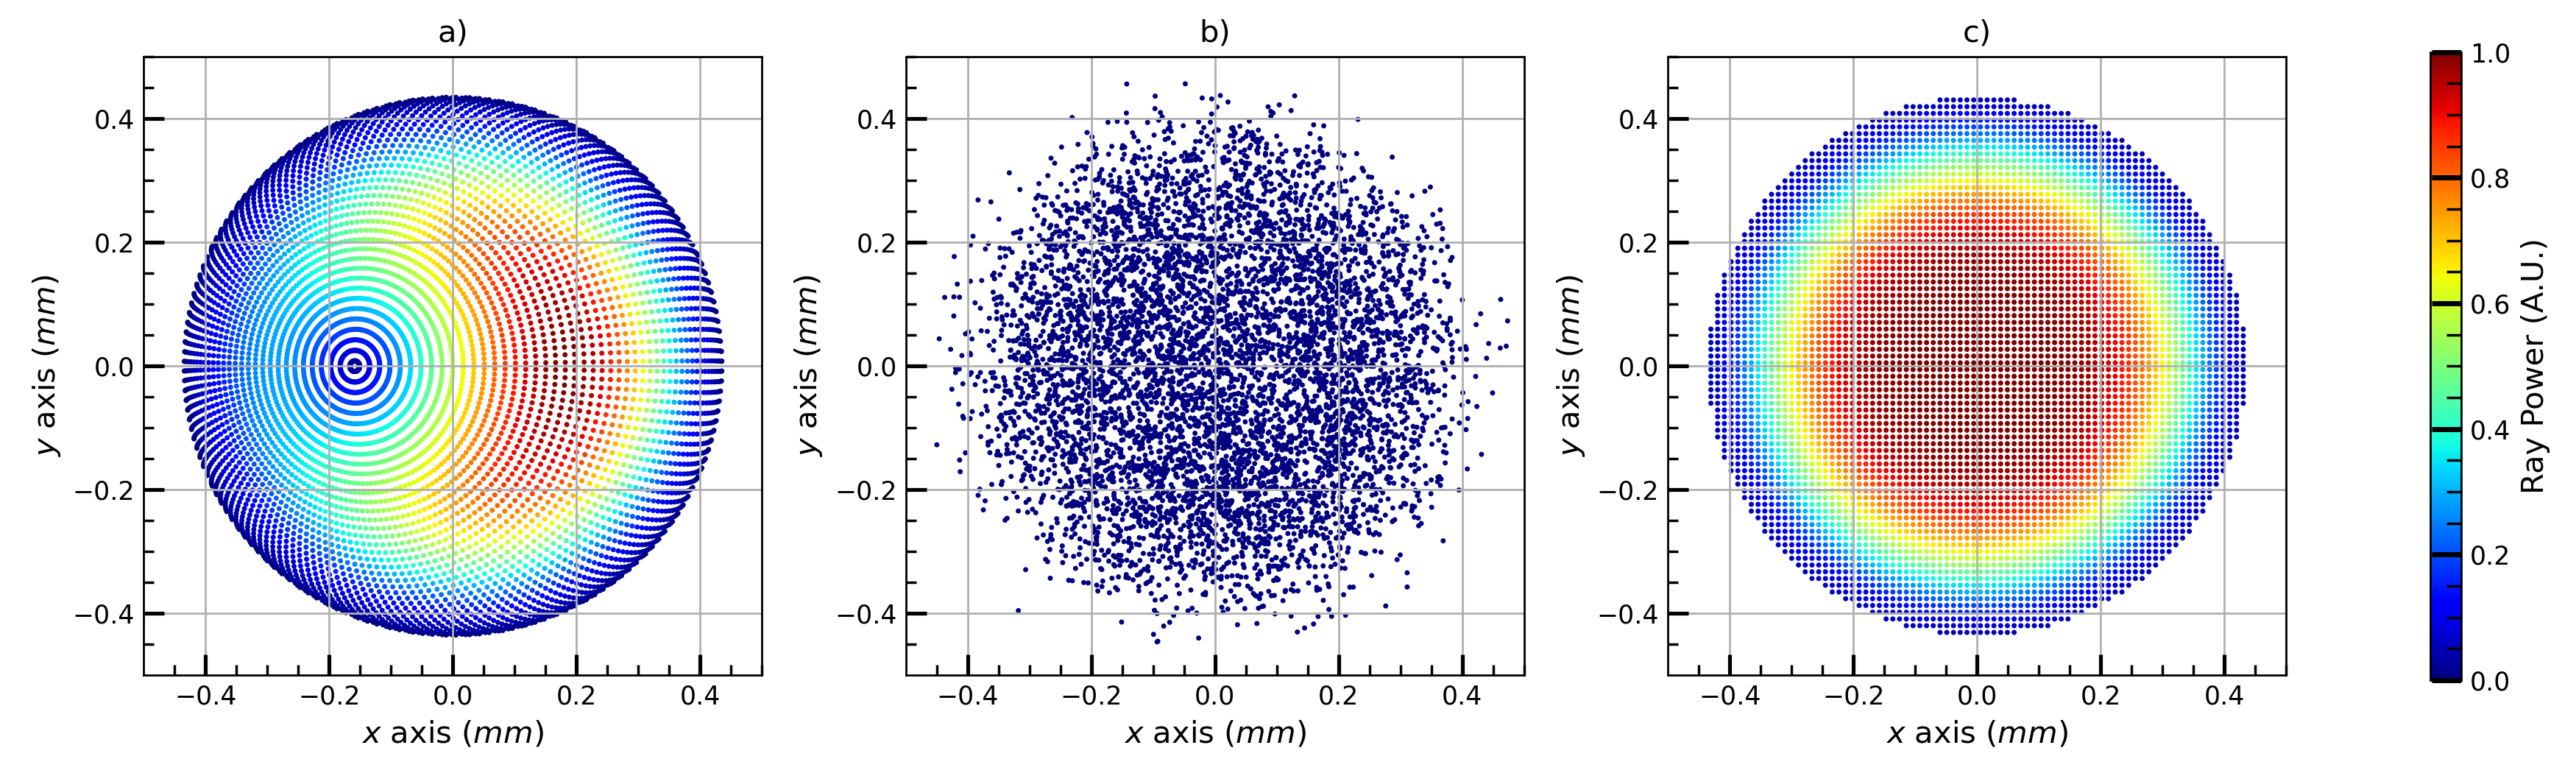
\includegraphics[width=\linewidth]{Numerics/Images/ray_init_plots.png}
    \centering
    \caption{Example initial locations for $\sim4000$ rays for an \textsc{Omega} beam port with super-Gaussian intensity profile, with a shape defined by $n_s=5.2$ and $\sigma=352\ \mu m$.
    The inverse-projection ray locations are shown in sub-figure a) which demonstrate a higher ray density for rays pointed to the pole at $x\sim\ -0.15 mm$.
    b) shows the randomly sampled rays where all rays are initialised with the same power, and c) shows uniformly sampled rays.}%
    \label{fig:SOLAS_ray_init}
\end{figure}

To obtain a noise-free energy deposition source term from a ray-trace, both the grid and choice of initial ray number and location is crucial.
The problems are closely related as a higher resolution grid requires a larger density of rays to get equivalent ray-per-cell statistics.
It is therefore wise to choose the number of rays used in a simulation to be some function of the grid used for the ray-trace.
Several methods for ray initialisation which have been implemented are briefly outlined here, along with a summary of their strengths and weaknesses.

All beams profiles described in this thesis have circularly symmetric super-Gaussian intensity profiles described by the equation,
\begin{equation}
    \label{eq:supgaus}
    I(r) = I_0 \exp{\Bigl( -\Bigl| \frac{r}{\sigma} \Bigr| ^{n_s} \Bigr)},
\end{equation}
where $r$ is the distance from the centre of the beam port, perpendicular to the beam normal, $I_0$ is the peak intensity, $\sigma$ is the beam width\footnote{The radius at which $I=I_0e^{-1}$.} and $n_s$ is the super-Gaussian exponent.

\paragraph*{Uniform Sampling}
In this method of ray initialisation, demonstrated in Fig.~\ref{fig:SOLAS_ray_init}.c, each beam is assigned a number of rays and a maximum initialisation radius\footnote{The maximum initialisation radius is usually set to be the radius at which $I=I_0e^{-3}$.}, beyond which rays are not initialised.
Rays are then placed on a uniform, square grid in this plane with a power proportional to the intensity value from by Eq.~\ref{eq:supgaus}.
For all three procedures described in this subsection, the total summed power of the rays is normalised to the incident beam power after the initialisation of all rays is complete.
Typically, for direct-drive, the total number of rays used for spherical simulations is chosen to be,
\begin{equation}
    \label{eq:SOLAS_nray_uniform}
    N_{\text{ray}} = C_{N}\max{(N_r N_{\varphi},N_r N_{\theta},N_{\theta} N_{\varphi})},
\end{equation}
where $N_{i=r,\varphi,\theta}$ is the number of \textsc{Solas} grid cells in each grid direction and $C_N$ is a user-parameter multiplier which to give better ray statistics for CBET simulations when required.
$C_N\sim 2$ is found to give converged deposition when including \ac{CBET} and so this value is used by default.

When there is sufficiently low ray-per-cell statistics, beat phenomena can occur between the ray spacing and the grid resolution.
In this event, especially when using a nearest neighbour interpolation for ray power deposition onto the grid, significant spurious modes can be introduced to the power deposition.
To resolve this, ray locations can be `dithered' so that they take a random position within the polygon\footnote{This polygon is a square for uniform sampling, but not for inverse-projection} defined by neighbouring ray locations.
This option is always used for simulations using uniform sampling in this thesis.

\paragraph*{Random Sampling}
Rays can also be randomly sampled according to the intensity profile.
Example ray locations from this method are shown in Fig.~\ref{fig:SOLAS_ray_init}.b.
Note that the intensity profile purely emerges from the ray locations in this method as all rays have equal power.
For no-\ac{CBET} simulations this is a useful method as it minimises coherent build-up of noise from ray-spacing, grid-resolution beating.
However, the wings of the intensity profile have poor ray statistics so for direct-drive \ac{CBET} calculations, resolving the reflected field and therefore the dominant backscatter \ac{CBET} is excessively expensive.

\paragraph*{Inverse-Projection}
Inverse-projection is the final method that has been implemented for ray initialisation in \textsc{Solas}.
The algorithm is described in detail in Appendix A of Ref.~\cite{marozas_wavelengthdetuning_2018}.
The method works by finding several surfaces, defined by fractions of the critical density and then creating aim points in each cell on the surface.
These aim points and their associated area on the surface are back-projected onto each beam port and rays are created if the aim point is not obscured by the surface on which it was created.
The power of the ray is then the back-projected area multiplied by the intensity at the beam port location.
For a spherical polar grid, this gives a ray distribution which varies in ray density according to which region on the beam port maps to regions on the grid with higher or lower cell-face areas.
The higher ray density region on the beam port maps to the polar region of the grid, at $x\sim -0.16\ mm$ on Fig.~\ref{fig:SOLAS_ray_init}.a have a correspondingly lower power compared to rays at equal radii to give the same intensity.

While inverse-projection does guarantee good ray statistics at given surfaces for the inbound component of the field, the algorithm does not extend to beyond ray caustics, or the reflected field component.
Therefore, ray statistics are not guaranteed to be good for the reflected field, so the advantages of this method are not evident for direct-drive \ac{CBET} simulations when backscatter must be resolved.
However, for no-\ac{CBET}, direct-drive simulations, this is a useful option for ray initialisation.

\paragraph*{}
For all simulations in this thesis, the uniform sampling method with ray dithering is used.
This method is found to give the best ray-per cell statistics across the semi-structured Eulerian grid described in Sec.~\ref{sec:SOLAS_mesh} while minimising the overall number of rays used required to resolve \ac{CBET}.

After rays are initialised on each of the beam ports, they are extrapolated to the edge of the computational domain.
Beam focussing is typically neglected, so all rays are assigned velocities parallel to the beam normal.
This approximation is widely used for codes that simulate \textsc{Omega}-scale direct-drive implosions, where the lasers are approximately collimated on the implosion scale~\cite{colaitis_inverse_2021,marozas_wavelengthdetuning_2018}.
It is assumed that outside of the simulation domain is vacuum and rays are therefore extrapolated to the edge of the computational domain in straight lines, using a simple root finding algorithm to obtain the intersection of the rays with either a spherical, cylindrical or rectangular domain depending on the simulation geometry.

%################################################################################
%################################################################################
\subsection{Equations of Rays and Adaptive Integration}%
\label{sec:SOLAS_ray_propagation}

The partial differential equations that are integrated along the trajectory of each ray are,
\begin{equation}
    \label{eq:SOLAS_rays}
    \begin{gathered}
        \frac{\text{d} \mathbf{x}}{\text{d} \tau}=\mathbf{k}, \\
        \frac{\text{d} \mathbf{k}}{\text{d} \tau}=\frac{1}{2} \nabla \varepsilon(\mathbf{x}), \\
        \frac{\text{d} \varphi}{\text{d} \tau}= \varepsilon(\mathbf{x}), \\
        \frac{\text{d} \omega}{\text{d} \tau}=\frac{\omega}{2 c} \frac{\partial\left(n_e / n_{\text{cr}}\right)}{\partial t}, \\
        \frac{\text{d} P}{\text{d} \tau}=-\kappa_{\text{IB}},
    \end{gathered}
\end{equation}
where $\varepsilon=1-n_e/n_{\text{cr}}$ is the dielectric permittivity of the plasma, $n_e$ and $n_{\text{cr}}$ are the electron and critical densities, $c$ is the speed of light, $t$ is time, $\kappa_{\text{IB}}$ is the \ac{Inv-Brem} absorption kernel, given explicitly in Eq.~\ref{eq:theory_inv_brem} and $\tau$ is the ray path length.
Note that the phase here is defined such that it has the same dimension as path length and therefore has spatial units.
The wavevector is normalised such that $|\vec{k}|=\sqrt{\varepsilon}$.
The optical path length is related to the arc length, $\text{d}s$ by the variable change $\text{d}s=\text{d}\tau\sqrt{\varepsilon}$.
In some formulations of the ray-tracing equations, the differential equations are written in terms of the arc length~\cite{marozas_wavelengthdetuning_2018,kaiser_laser_2000}, which is equivalent, but more complicated and without benefit.
Note that the time, $t$ is not related to the ray path length $\tau$, because an operator split approach is taken to the ray-trace, such that the hydrodynamic variables are frozen and the ray-trace finds the time independent trajectory of the light through these profiles.
The path length $\tau$ is therefore best seen as a parameterisation of the ray curve.

The frequency shift arises due to light propagating through a time varying refractive index.
This causes successive wavefronts to bunch up (blue-shift) or rarefy (red-shift), which occurs for a temporally increasing or decreasing $n_e$ respectively \cite{dewandre_doppler_1981}.
This effect is only significant for the work presented in this thesis when calculating \ac{CBET}.
For direct-drive calculations at the \textsc{Omega} laser facility scale, this results in wavelength shifts of $\Delta \lambda/\lambda_0 \sim \mathcal{O}(0.1\%)$, which is typically negligible for computing ray trajectories.
However, the induced wavelength shift is relatively significant when calculating the \ac{CBET} resonance and in direct-drive can alter the spatial location where scattering is significant~\cite{colaitis_inverse_2021}.
Neglecting time-dependent ionisation effects, which is a good assumption during peak-power for the approximately steady-state direct-drive corona where \ac{CBET} occurs, the time derivative can be obtained by assuming that $n_e$ is advected with the bulk fluid,
\begin{equation}
    \label{eq:SOLAS_doppler}
    \frac{\partial\left(n_e / n_{\text{cr}}\right)}{\partial t} = - \frac{ \iiint_V \ \nabla.[(n_e/n_{\text{cr}})\vec{u}] \ \text{d}V }{ \iiint_V \text{d}V },
\end{equation}
where $\vec{u}$ is the fluid velocity and the integral is over a computational cell volume.
Using the Divergence Theorem, this can be rewritten,
\begin{equation}
    \label{eq:SOLAS_doppler_used}
    \frac{\partial\left(n_e / n_{\text{cr}}\right)}{\partial t} = - \frac{ \closediint_S \ (n_e/n_{\text{cr}})\hat{\vec{n}}.\vec{u} \ \text{d}S }{ \iiint_V \text{d}V },
\end{equation}
where the integral on the numerator is now over the cell bounding area, with normal $\hat{\vec{n}}$ \cite{marozas_wavelengthdetuning_2018}.

Two algorithms have been implemented to integrate Eqs.~\ref{eq:SOLAS_rays}, an adaptive RK45 algorithm and the Kaiser algorithm.
These are described below, alongside the method for ray-deposition-to-cell interpolation and time-stepping considerations.

\paragraph*{Adaptive RK45 Algorithm}
The default ray evolution algorithm in \textsc{Solas} is to solve Eq.~\ref{eq:SOLAS_rays} using an adaptive RK45 algorithm with stepsize control~\cite{press_numerical_2007}.
Ray steps are either limited by the error from this algorithm, or by distance to the next impact with a cell face.
Evaluations of the right-hand side of these equations employ trilinear interpolation for $n_e$, $\nabla n_e$ and $T_e$ to obtain varying values for these quantities at different locations throughout the cell.
All other quantities are either defined at the ray location, or use nearest neighbour interpolation.
The \texttt{bspline-fortran} library has also been implemented to allow tricubic interpolation of $n_e$, which yields a quadratically varying $\nabla n_e$ across the grid~\cite{williams_bsplinefortran_2024}.
This is slow to evaluate many times per ray step as is required in an RK45 algorithm and therefore limits performance, but is used throughout this chapter as a higher order solution to validate accuracy of the default interpolation.

Linear interpolation of $n_e$ and $T_e$ is required for accurate computation of $\kappa_{\text{IB}}$, especially for `cold-start' simulations where light impacts upon a solid target and the plasma profiles have steep gradients.
Interpolation of $\nabla n_e$ was found to be necessary to obtain low-noise ray amplitudes from neighbouring rays for \ac{CBET} evaluation, which is described in more detail in~\ref{sec:SOLAS_field_reconstruc}.
Linear interpolation of both $n_e$ and $\nabla n_e$ is technically inconsistent, because $\nabla n_e$ should be the gradient of $n_e$, however the test cases presented in Sec.~\ref{sec:SOLAS_ray_validation} found that this did not reduce accuracy compared to the Kaiser algorithm, which employs a self-consistent linear interpolation of $n_e$ and constant $\nabla n_e$ within a computational cell.

\paragraph*{Kaiser Algorithm}
The Kaiser algorithm for ray integration has also been implemented~\cite{kaiser_laser_2000}.
In this algorithm, each cell has a single $\nabla n_e$ and an $n_e$ value defined at the cell centre, allowing for linear interpolation of $n_e$ throughout the cell.
In a constant $\nabla n_e$ region, the trajectory of rays can be analytically shown to follow a parabola.
The Kaiser algorithm thus evolves rays over parabolic segments between cells by finding the intersection of the parabola with cell faces, using a root finding algorithm.
Assuming constant $\nabla n_e$ cells leads to discontinuities in $n_e$ at cell interfaces when the true gradient is not linear and thus Snell's Law is used to refract rays upon cell exit.
While this method is often slightly more efficient compared to the adaptive RK45, it was found that when attempting to reconstruct the ray amplitude from the area of neighbouring rays, as outlined in Sec.~\ref{sec:SOLAS_field_reconstruc}, excessive noise was introduced in the amplitude from the discontinuous refraction.
Therefore, the adaptive algorithm was used for all work in this thesis, other than where explicitly outlined.

\begin{figure}[t!]
    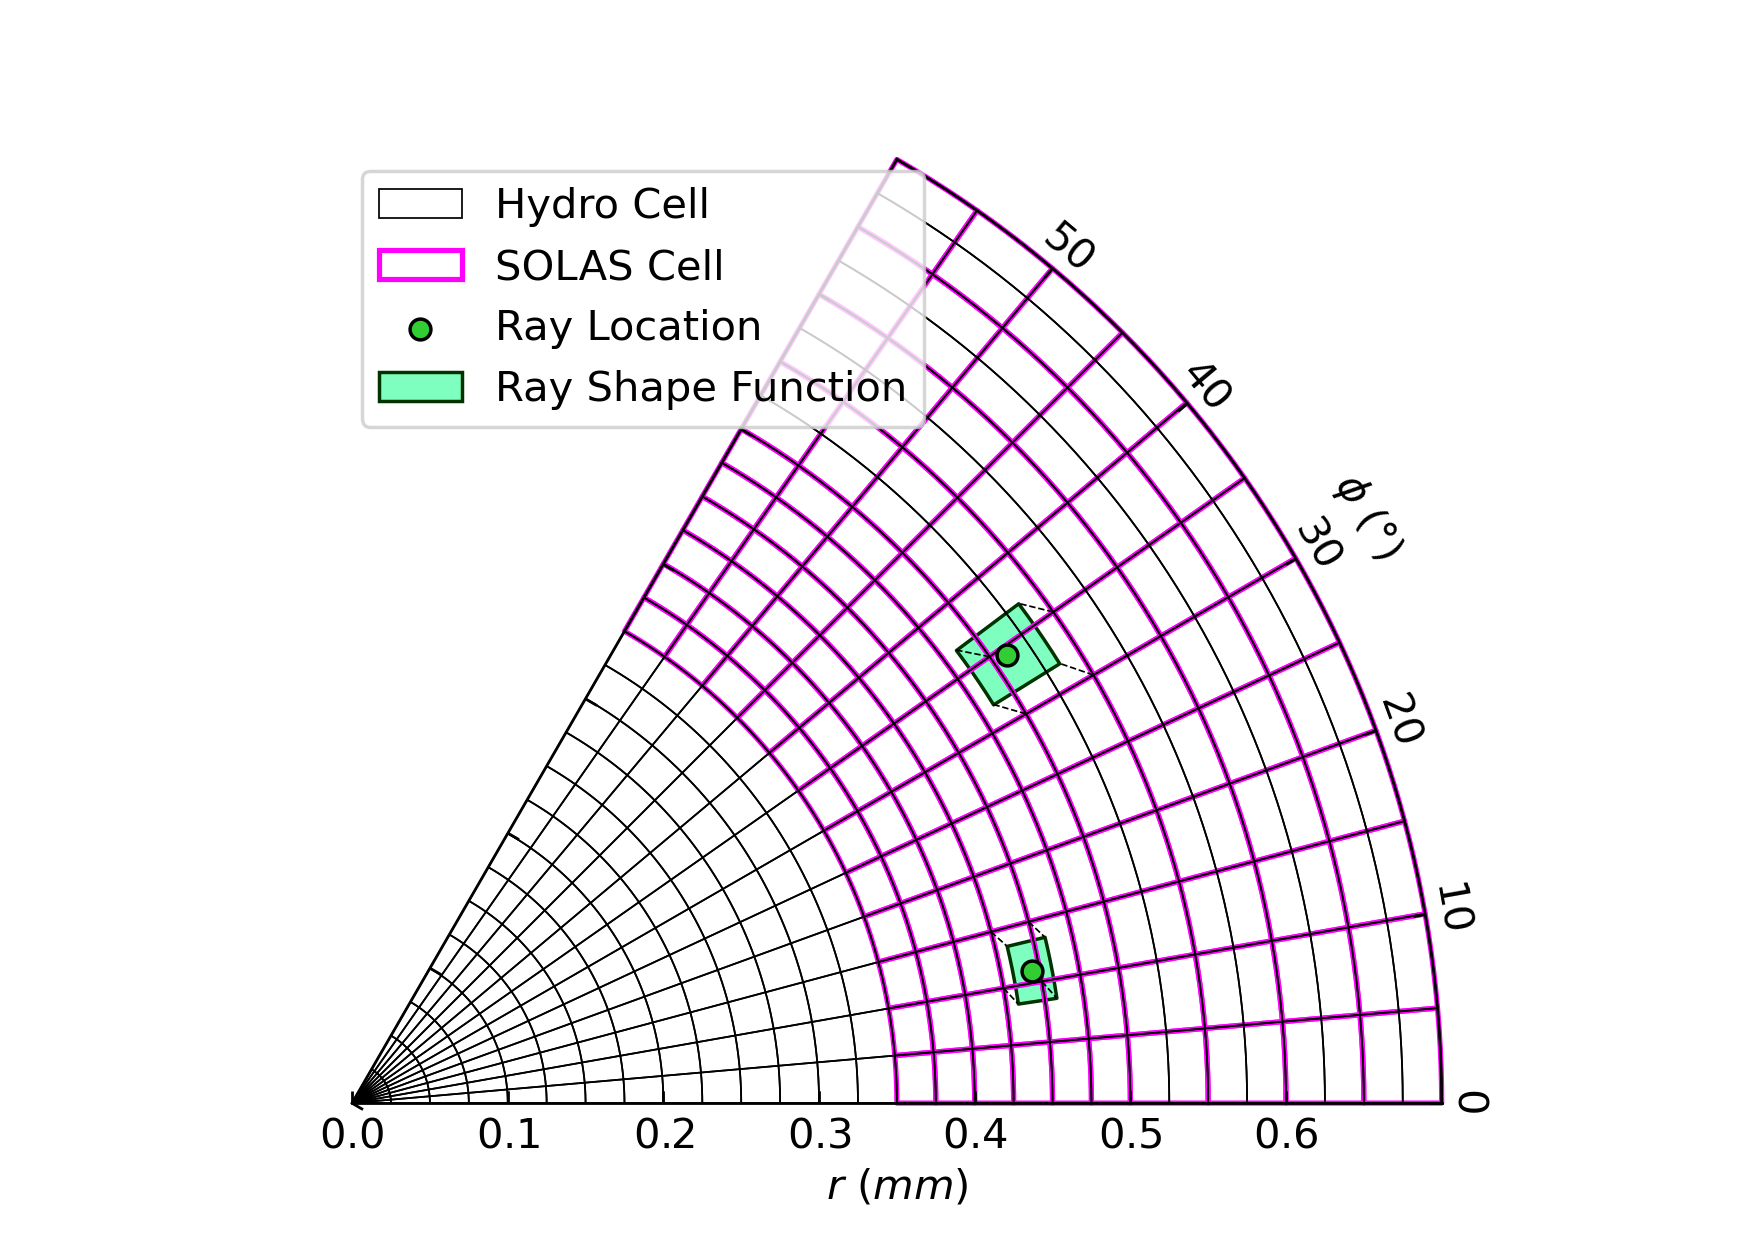
\includegraphics[width=10.0cm]{Numerics/Images/SOLAS_ray_shape_functions.png}
    \centering
    \caption{Shape function smearing for ray power interpolation to the \textsc{Solas} grid for a cylindrical mesh.
    The shape function has the same size and geometry as the \textsc{Solas} grid cell which the ray is located in.
    A top-hat shape function is used, so the fraction of the deposited power interpolated to a given cell is proportional to the volume overlap of the shape function with the cell.}%
    \label{fig:SOLAS_ray_shapefunction}
\end{figure}

\paragraph*{Shape Functions for Ray Deposition}
Nearest neighbour interpolation of power deposition, which is defined along the ray trajectory, onto the computational grid can result in significant levels of noise in the power deposition profile when ray statistics are not sufficiently high.
This is similar to problems experienced in \ac{PiC} codes when interpolating macro particles to the grid without the use of shape functions~\cite{birdsall_plasma_1985,arber_contemporary_2015}.
A \ac{PiC}-inspired shape function approach was therefore taken, where the power deposition from rays is smeared across neighbouring cells.
A top hat shape function is used, with a shape function that has the size and shape of the cell that the ray is located within, as is shown in Fig.~\ref{fig:SOLAS_ray_shapefunction}.
The power deposited into each cell that has an overlap with the shape function bounds is therefore proportional to the volume overlap of the shape function with the cell.
This approach is more explicitly outlined, particularly for the case of the non-logically rectilinear grids which are present for \textsc{Solas}, in Ref.~\cite{cornet_new_2007}.
This smearing is somewhat numerically diffusive and therefore can be optionally disabled.
For the work presented in this thesis, the shape function smearing is employed for multidimensional direct-drive simulations, but otherwise disabled.

\paragraph*{Hydrodynamic Time Step Limiter}
Laser heating of a plasma results in a temperature increase of the material, which also reduces the \ac{Inv-Brem} kernel.
If the hydrodynamic timestep, $\delta t$ is too large, excessive heating occurs in initially cold cells, which should have the magnitude of absorption gradually reduced as they warm up.
This can lead to spurious oscillations in temperature at fine grid resolutions.
A limiter on the hydrodynamic time-step is therefore introduced to prevent large heating in any cell within one timestep.
The limit detailed by Haines in Ref.~\cite{haines_coupling_2020} is enforced, which estimates the increase in temperature of a cell from \ac{Inv-Brem} heating by assuming an ideal gas equation of state to derive,
\begin{equation}
    \label{eq:SOLAS_dt_limit}
    \delta t = \min_{n\in \text{cells}}{\left( \tilde{\delta t}, C_{\delta t} \frac{3}{2} \frac{n_{e,n} e T_{e,n} V_n }{P_n} \right)},
\end{equation}
where $\tilde{\delta t}$ is the stable hydrodynamic timestep from other physical processes, $n_{e,n}$, $T_{e,n}$, $V_n$ and $P_n$ are the electron density, electron temperature, volume and deposited power into cell $n$, and $C_{\delta t}$ is a user defined stability parameter.
By default, the parameter $C_{\delta t}$ is set to 1, which is found to be adequate for most situations~\cite{haines_coupling_2020}.
Note that Eq.~\ref{eq:SOLAS_dt_limit} is only applied in cells where $n_{e,n}>1\times 10^{-4} n_{\text{cr}}$.
Small amounts of deposition in these cells can lead to large temperature increases, which severely limits $\delta t$, despite the cells often being far from the region of interest, normally near critical, where the maximum deposition occurs.
For simulations where a laser heats a solid, initially cold target, Eq.~\ref{eq:SOLAS_dt_limit} mostly only affects the hydrodynamic timestep early in the simulation, after which the laser-heated plasma corona remains in a mostly steady-state unless there are steep changes in incident power.

%##################################################
\subsubsection{Ray Solver Validation}%
\label{sec:SOLAS_ray_validation}

Several validation problems have been conducted to verify that the ray solver has been implemented correctly.
Here the quadratic trough and cylindrical helix test problems are presented, which compare the path of a single ray in to an analytic solution in order to verify that the ray solvers correctly obtain the trajectory of light.
The blast wave problem is also presented which is a test of \ac{Inv-Brem} absorption to an analytic solution in the absence of thermal conduction and hydrodynamic motion.

\paragraph*{Quadratic trough}

\begin{figure}[t!]
    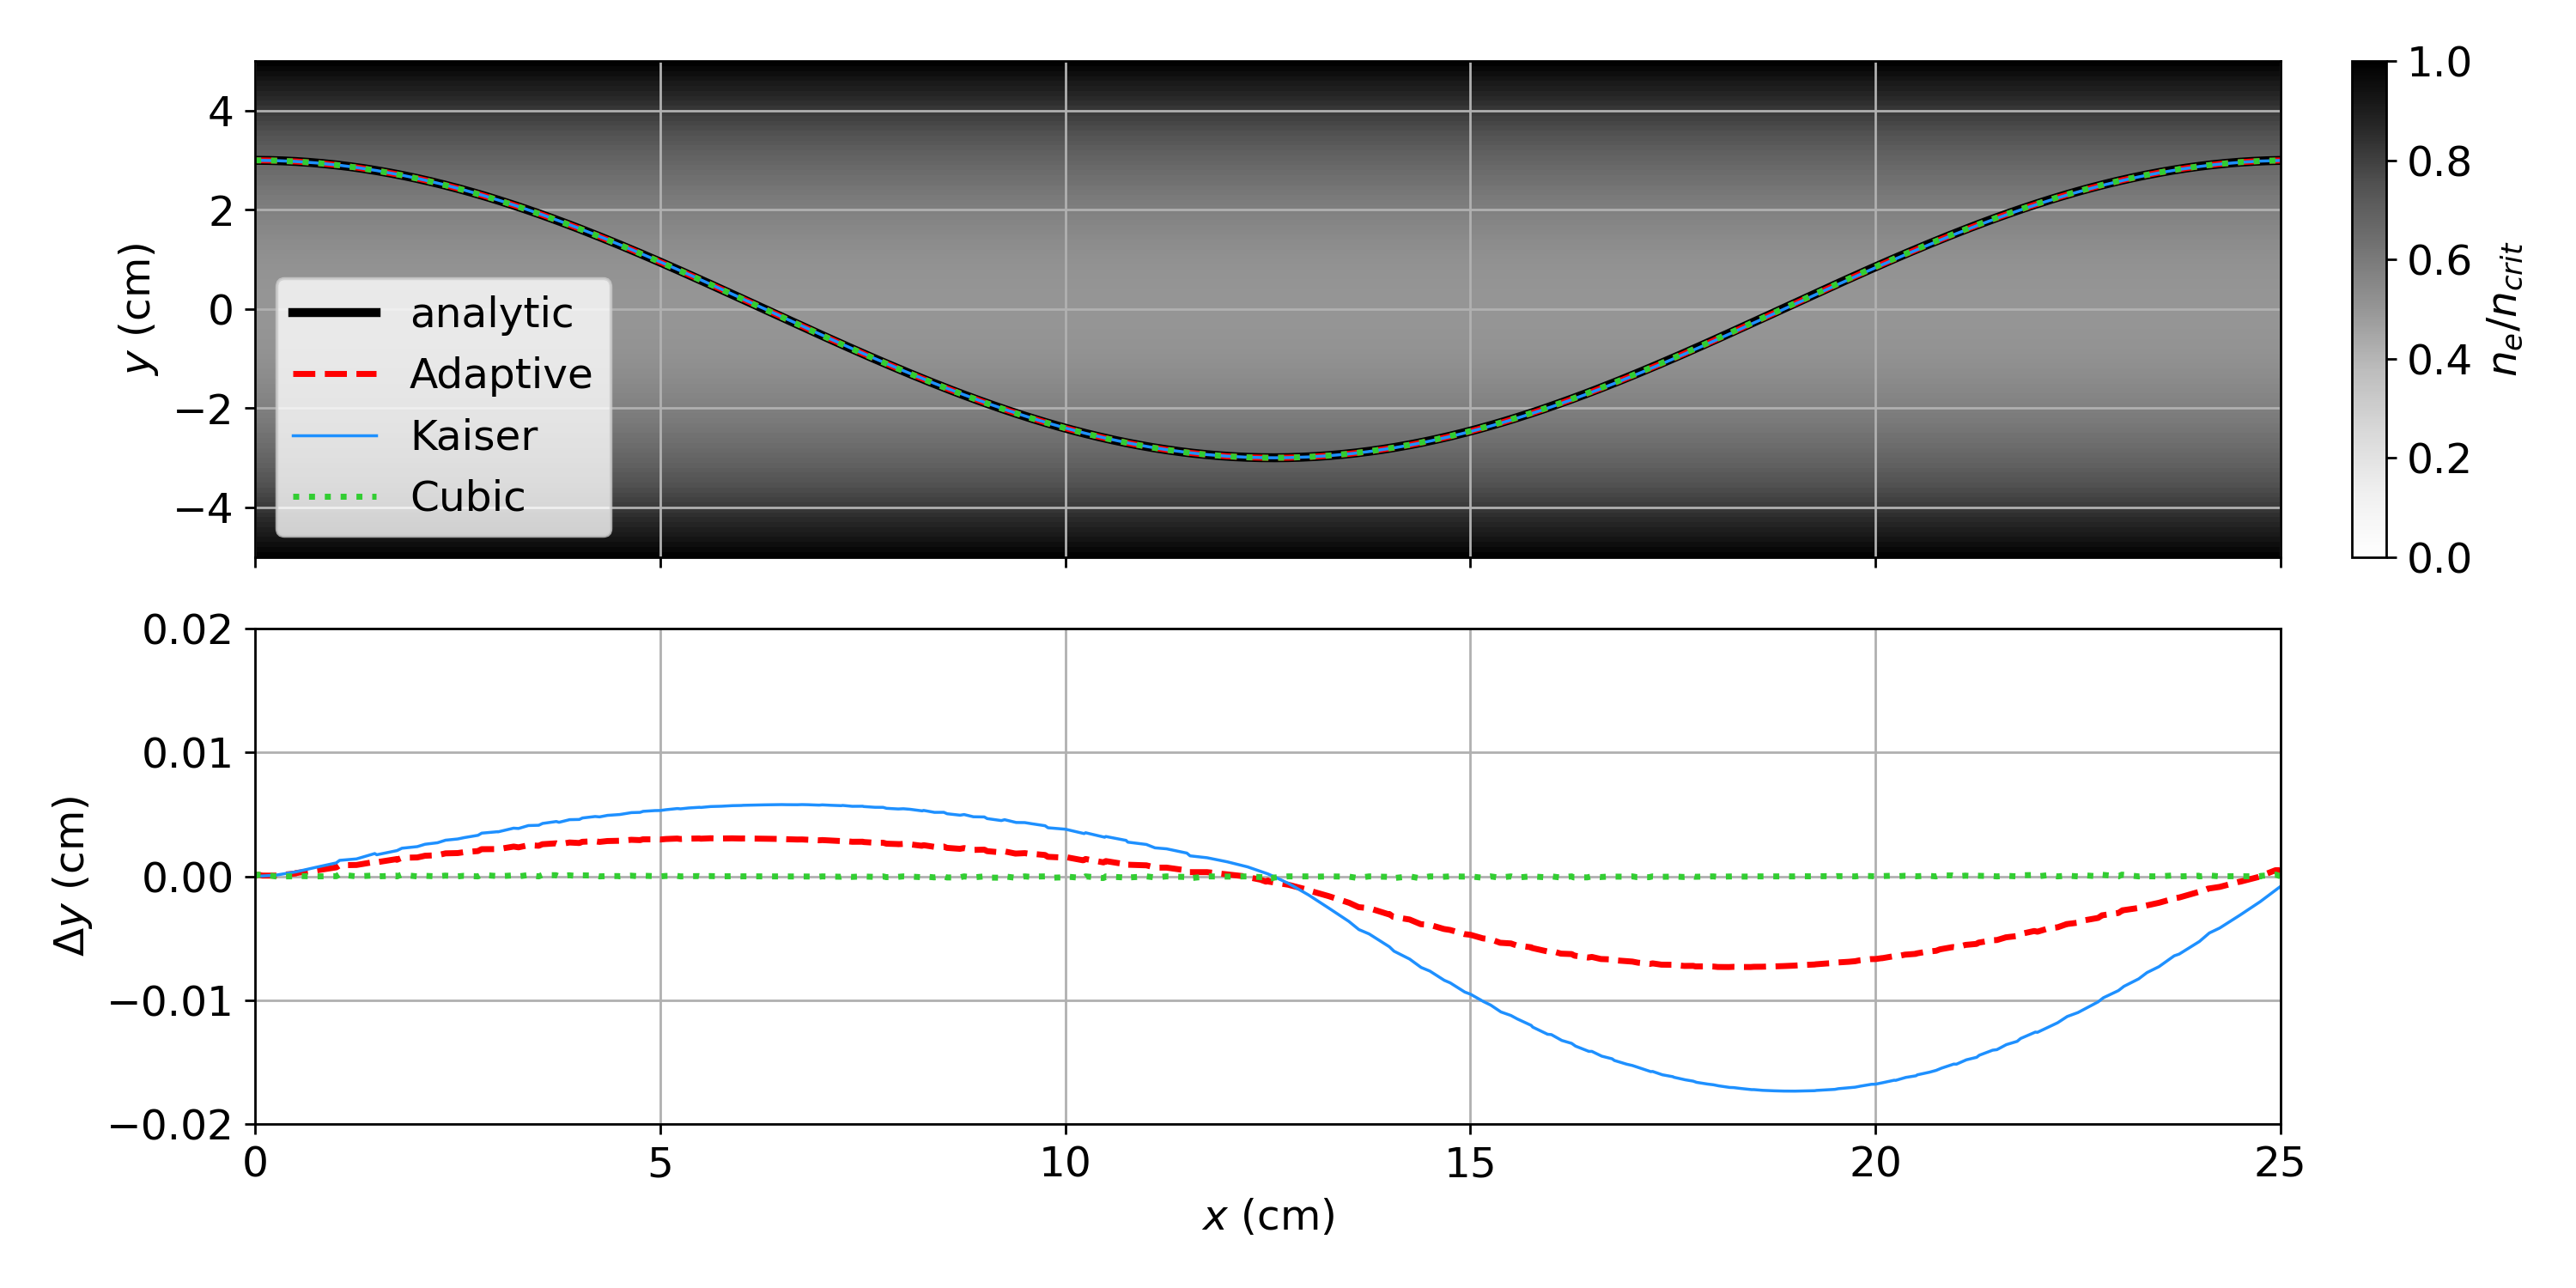
\includegraphics[width=\linewidth]{Numerics/Images/Quadtrough.png}
    \centering
    \caption{Results of the quadratic trough ray trajectory test problem for the adaptive solver with 3 different cases.
    These are default settings (linear interpolation of both $n_e$ and $\nabla n_e$), the Kaiser algorithm (linear interpolation of $n_e$ and uniform $\nabla n_e$ in a cell) and the adaptive algorithm with tricubic interpolation of $n_e$).
    The top plot shows ray trajectories and analytic trajectory and the bottom plot shows absolute errors for the 3 cases.}%
    \label{fig:SOLAS_quadtrough}
\end{figure}

The quadratic trough is a test of ray trajectory in a quadratic density trough, which admits an analytic solution of a periodically oscillating ray~\cite{kaiser_laser_2000,haines_coupling_2020}.
The density profile used for the test is defined as,
\begin{equation}
    n_e(y) = \frac{n_{\text{cr}}}{2} \left( 1 + \frac{y^2}{y_c^2} \right),
\end{equation}
which for light with wavelength $\lambda=351\ \text{nm}$, is initialised with $n_{\text{cr}} = 9.049\times 10^{21} \ \text{cm}^{-3}$ and $y_c = 5 \ \text{cm}$.
The domain has bounds $x \in [0,25]\ \text{cm}$ and $y \in [-5,5]\ \text{cm}$ and a ray enters the domain at $[x_0,y_0]=[0,3]\ \text{cm}$.
Analytic integration of the first 2 lines from Eq.~\ref{eq:SOLAS_rays}, yields the analytic trajectory as a function of ray path length, $\tau$,
\begin{equation}
    \begin{gathered}
        x(\tau) = \tau\sqrt{1-\frac{n_e(y_0)}{n_{\text{cr}}}}, \\
        y(\tau) = y_0\cos{\left( \frac{\tau}{\sqrt{2}y_c} \right)}.
    \end{gathered}
\end{equation}

The analytic trajectory is compared to the solution from the adaptive solver (using both default interpolation and tricubic interpolation of $n_e$) and the Kaiser algorithm in Fig.~\ref{fig:SOLAS_quadtrough}.
The associated error, defined as the difference in $y$ from the analytic value at a given $x$ is also plotted.
Note that all results were obtained using a grid resolution of $100\times100$ cells.
The top panel demonstrates that all trajectories are identical to the analytic solution by eye.
The corresponding errors show that the tricubic interpolation effectively perfectly recreates the analytic solution and the Kaiser error is slightly more significant compared to the default adaptive error.
The tricubic error is insignificant because the cubic interpolation perfectly recreates the true density profile, so the errors are purely numeric, not due to the resolution.
Errors from the other algorithms would therefore decrease more quickly with increasing resolution as the density profile the ray sees becomes more similar to a quadratic trough.
The error from the default adaptive interpolation (linear interpolation of both $n_e$ and $\nabla n_e$) is lower than that of Kaiser (linear $n_e$ and uniform $\nabla n_e$), indicating that the inconsistent interpolation is not a significant issue for resolving ray trajectories.

\paragraph*{Cylindrical-Helix}

\begin{figure}[t!]
    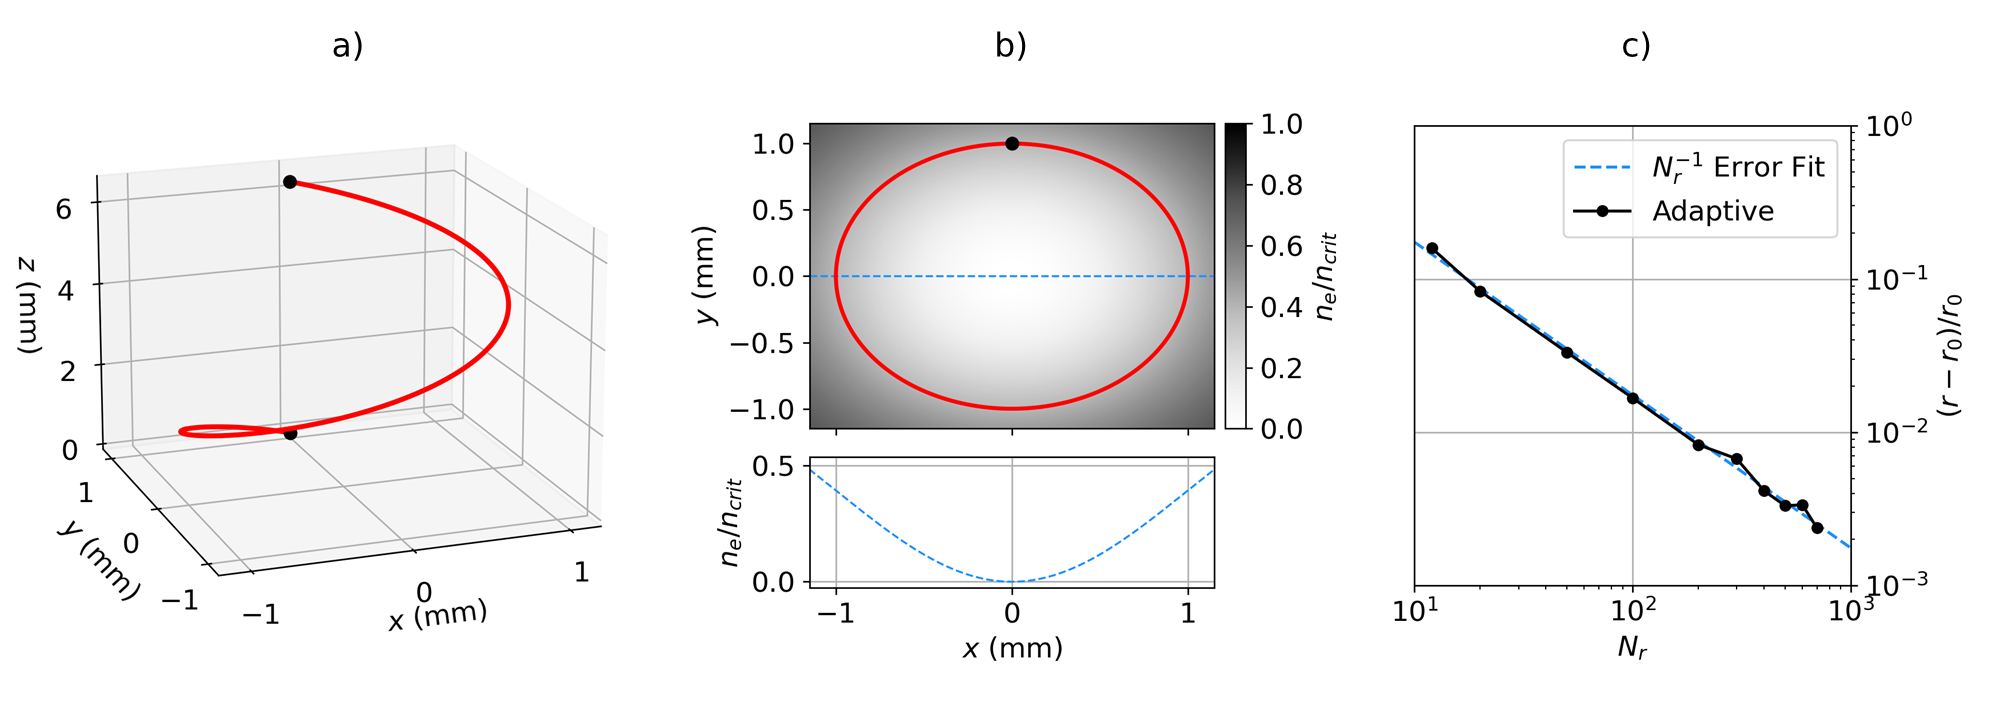
\includegraphics[width=\linewidth]{Numerics/Images/cyl_helix.png}
    \centering
    \caption{Results from the cylindrical-helix test problem, obtained using the default adaptive RK45 algorithm.
    a) shows the trajectory of a ray from a simulation with 100 radial cells in 3-D space.
    b) shows the trajectory of the ray projected on the $x-y$ plane, along with the $n_e$ profile.
    c) shows the error of the test, defined as the fractional difference in radius of the ray as it exits the domain from the initial radius, as a function of number of radial cells.}%
    \label{fig:SOLAS_cylhelix}
\end{figure}

The quadratic trough test ensures that the ray evolution algorithm functions correctly in Cartesian geometry.
An additional test was desired in non-Cartesian geometry, because \textsc{Chimera} also operates with cylindrical and spherical grids.
The cylindrical-helix test was therefore devised, where a ray enters an axially symmetric density trough that keeps the ray at a constant, cylindrical radius, $r$, as is shown in Fig.~\ref{fig:SOLAS_cylhelix}.b.
As is shown in Fig.~\ref{fig:SOLAS_cylhelix}.a, the $z$ extent of the simulation is chosen such that the ray has performed one complete helical spiral when it exits the domain.
By requiring that a ray undergo circular motion in the $x-y$ plane and specifying the initial ray direction such that $k_{z0}=\sqrt{k_{x0}^2+k_{y0}^2}$, it can be derived that a ray entering the domain at $r_0$ will undergo one complete helical spiral over a $z$ length $\Delta z= 2\pi r_0$, if the density profile has the shape,
\begin{equation}
    \label{eq:SOLAS_cyl_helix_ne}
    n_e(r) = n_{\text{cr}} \left( 1-\exp{\left( \frac{-r^2}{2r_0^2} \right)} \right).
\end{equation}
For a ray entering the domain at $[x_0=0,\ y_0=1,\ z_0=2\pi]$ mm, with initial wavevector $[k_{x0}=\sqrt{\varepsilon_0/2},\ k_{y0}=0,\ k_{z0}=-\sqrt{\varepsilon_0/2}]$, the ray position as a function of path length $\tau$ is,
\begin{equation}
    \begin{gathered}
        x(\tau) = r_0\sin{\left( \sqrt{\frac{\varepsilon_0}{2}}\tau \right)}, \\
        y(\tau) = r_0\cos{\left( \sqrt{\frac{\varepsilon_0}{2}}\tau \right)}, \\
        z(\tau) = z_0 - \sqrt{\frac{\varepsilon_0}{2}}\tau,
    \end{gathered}
\end{equation}
where $\varepsilon_0\equiv\varepsilon(r=r_0)$.

This problem was run in cylindrical geometry for a variety of radial resolutions, employing the default adaptive RK45 solver with linear interpolation of both $n_e$ and $\nabla n_e$.
The domain bounds for the problem were $r \in [0,1.5]\ \text{mm}$, $\varphi \in [0,2\pi]$ and $z \in [0,2\pi]\ \text{mm}$, with a single cell in both the $\varphi$ and $z$ directions.
For all radial resolutions, the ray was observed by eye to exit the domain at the expected location, verifying that the ray-trace is functional in non-Cartesian geometries.
Plotting the fractional error in ray exit location as a function of number of radial cells, $N_r$ in Fig.~\ref{fig:SOLAS_cylhelix}.c, demonstrates that the error in final position of the ray scales as $N_r^{-1}$.
This is because larger $N_r$ more closely recreates the density profile in Eq.~\ref{eq:SOLAS_cyl_helix_ne}.
The error scaling in dictated by the lowest order interpolation used in the algorithm.
This is the linear interpolation of $n_e$ for the default adaptive RK45 solver, which leads to the $N_r^{-1}$ scaling.

\paragraph*{Blast wave}

\begin{figure}[t!]
    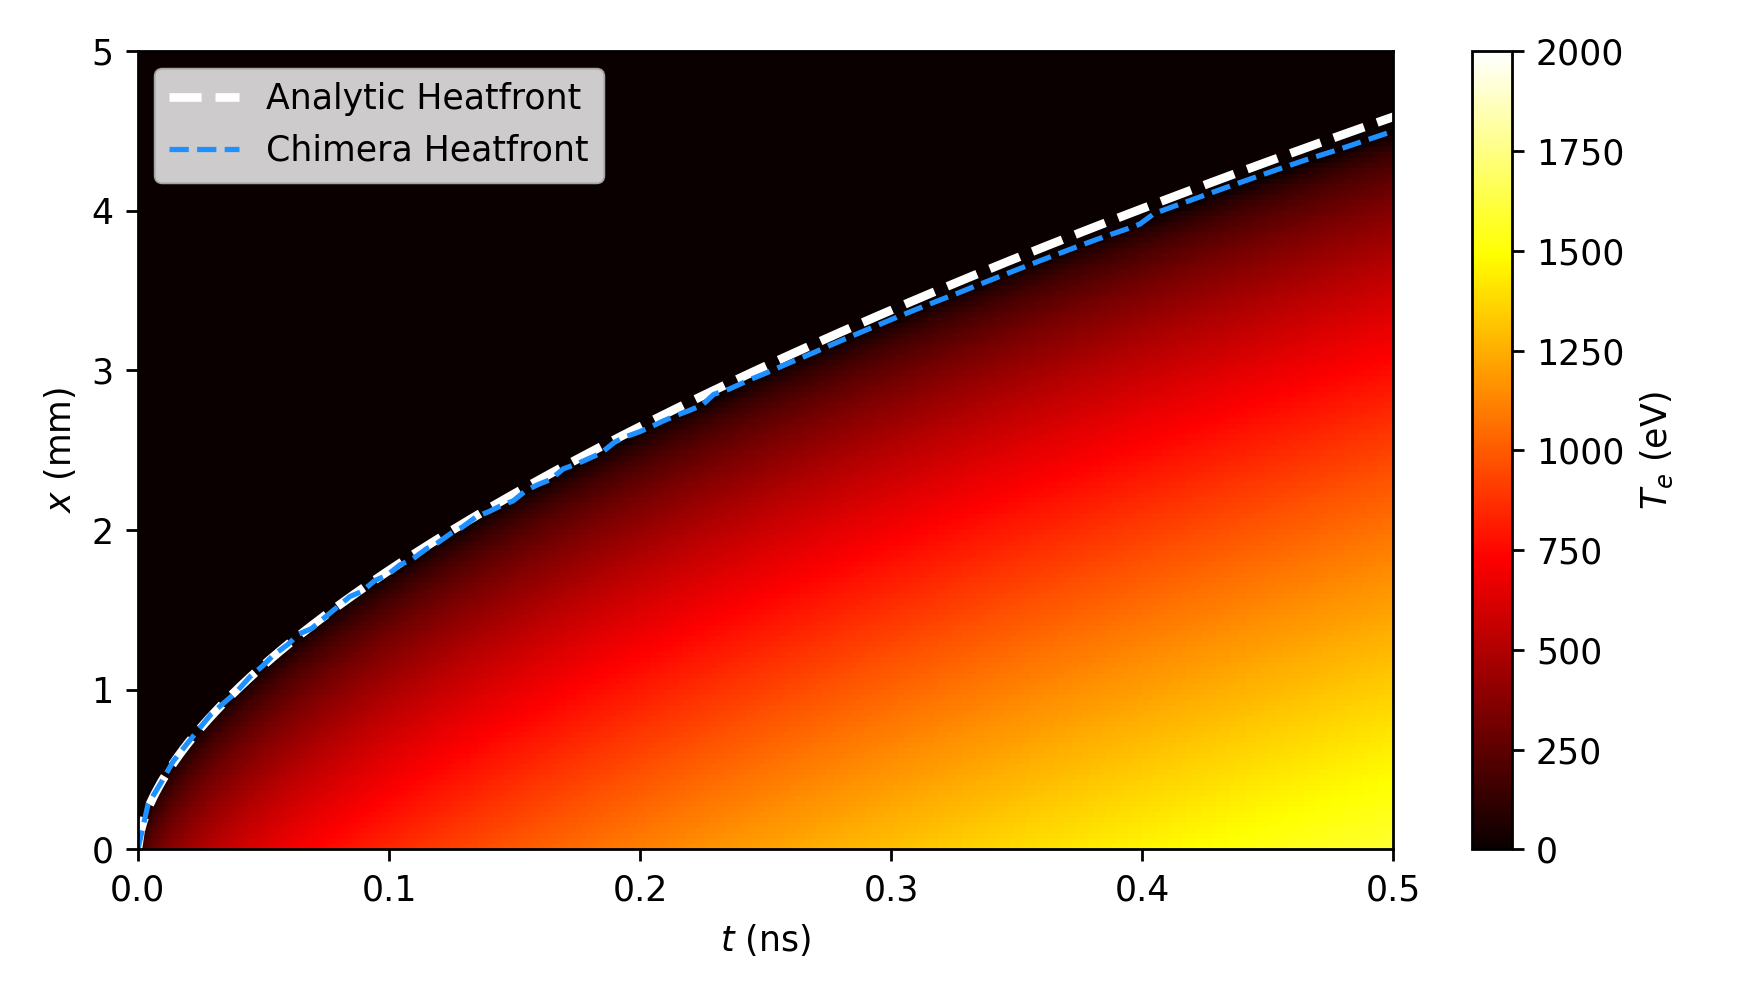
\includegraphics[width=0.9\linewidth]{Numerics/Images/blastwave.png}
    \centering
    \caption{Results of the blast wave \ac{Inv-Brem} absorption test problem.
    The colour-plot shows the temperature of the 1-D simulation as a function of time ($x$-axis) and space ($y$-axis).
    The heatfront obtained from \textsc{Chimera}, which is the maximum $x$ location where $T_e>T_{e0}$, is in good agreement with the analytic solution.}%
    \label{fig:SOLAS_blastwave}
\end{figure}

The blast wave problem is a validation test of the implementation of \ac{Inv-Brem} absorption~\cite{denavit_laser_1994,haines_coupling_2020}.
In this problem, a $527\ \text{nm}$, $2\ \text{ns}$ laser is incident on a uniform density $(\rho = 1\ \text{mg}/\text{cm}^{-3})$, cold gas $(T_{e0} = 1\ \text{eV})$ with fixed ionisation at $Z=6$, that has an ideal gas equation of state.
The $\ln{\Lambda}$ value used for the $\kappa_{\text{IB}}$ coefficient is fixed at 7.
The laser travels in the $x$ direction and has an intensity of $6.4\times 10^{13}\ \text{Wcm}^{-2}$.
Hydrodynamic motion and transport is disabled in the simulation.
The laser is initially strongly absorbed in the gas, so energy is not transported beyond the initial layer, perpendicular to the laser propagation direction.
As the gas heats up, $\kappa_{\text{IB}}$ decreases and therefore more energy is transported further into the domain by the laser, moving the heatfront forward.
The heatfront $x_{\text{analytic}}(t)$, defined as the largest $x$ coordinate at a time, $t$ where $T_e>T_{e0}$, has an analytic solution, derived by Denavit and Phillion in Ref.~\cite{denavit_laser_1994},
\begin{equation}
    x_{\text{analytic}}(t) = \frac{2}{3\kappa_{\text{IB}}}\left( \frac{5}{3} \frac{\kappa_{\text{IB}}I}{n_e k_B} \right)^{3/5},
\end{equation}
which can be compared to the result from a ray-tracing simulation.

Fig.~\ref{fig:SOLAS_blastwave} shows the results for $T_e(x,t)$ and the heatfront location from a \textsc{Chimera}-\textsc{Solas} simulation of the blast wave problem.
The heatfront from the simulation compares well to the analytic heatfront, validating the implementation of the \ac{Inv-Brem} absorption kernel.


%###############################################################################################################################
%###############################################################################################################################
%###############################################################################################################################
\section{Ray-Based Field Reconstruction and Ray Sheets}%
\label{sec:SOLAS_field_reconstruc}

In order to compute \ac{CBET}, or other \ac{LPIs} in a ray-tracing calculation, additional information about the electric field or intensity of the light is required than can be obtained from the ray directly.
This section outlines the method used in \textsc{Solas} to obtain the electric field of the light along the path of each ray, which broadly follows the implementation from Ref.~\cite{follett_validation_2022}.

%################################################################################
%################################################################################
\subsection{Ray-Amplitude and Field Estimate from Neighbour-Rays}%
\label{sec:SOLAS_ray_amplitude}

\begin{figure}[t!]
    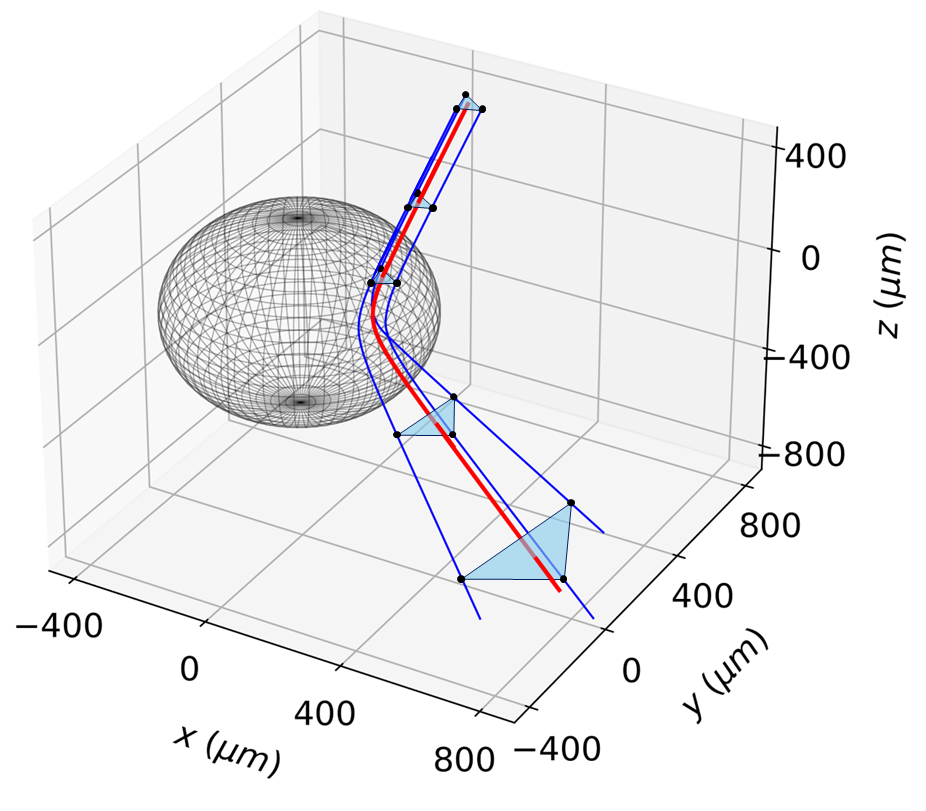
\includegraphics[width=0.75\linewidth]{Numerics/Images/3d_raytube.png}
    \centering
    \caption{A 3-D illustration of the ray-amplitude construction for a single ray in a spherically-symmetric, direct-drive like plasma profile.
    The critical surface is shown as the grey wire mesh.
    The main-ray trajectory is plotted in red, and its three neighbour-ray trajectories are in blue.
    The area of the main-ray at 5 successive phase-fronts is plotted, \textit{i.e.} when the main- and neighbour-rays all have the same phase, $\varphi$, is illustrated by the shaded triangles.
    This is inversely proportional to the ray-amplitude at this location.}%
    \label{fig:SOLAS_3draytube}
\end{figure}

Recalling the formula for the ray-amplitude, $A$, Eq.~\ref{eq:theory_rayamp} from Sec.~\ref{sec:theory_rayamp},
\begin{align}
    A(\tau) = A(0)\left| \frac{D(0)}{D(\tau)} \right|^{1/2}, &&
    D(\tau) = 
    \begin{bmatrix}
        \frac{\partial x}{\partial \zeta_1} & \frac{\partial x}{\partial \zeta_2} & \frac{\partial x}{\partial \tau} \\
        \frac{\partial y}{\partial \zeta_1} & \frac{\partial y}{\partial \zeta_2} & \frac{\partial y}{\partial \tau} \\
        \frac{\partial z}{\partial \zeta_1} & \frac{\partial z}{\partial \zeta_2} & \frac{\partial z}{\partial \tau}
    \end{bmatrix},
\end{align}
where $[x,y,z]$ and $[\zeta_1,\zeta_2,\tau]$ are the ray real-space and phase-space coordinates respectively and $D$ is the Jacobian for the coordinate transform from phase-space to real-space.
When refraction forces rays closer together, $|D(\tau)|$ will decrease and equally, when refraction forces rays to separate, $|D(\tau)|$ will increase.
The amplitude can therefore be approximated by assuming proportionality between the determinant of the Jacobian and the area, $S$ of an infinitesimally small bundle of rays surrounding the main-ray,
\begin{equation}
    A(\tau) = \varepsilon^{-1/4} \sqrt{\frac{S(\tau=0)}{S(\tau)}},
\end{equation}
where the $\varepsilon^{-1/4}$ term accounts for swelling of the field due to the increased optical path through plasma with finite density~\cite{follett_validation_2022}.
Note that the amplitude is a purely geometric quantity, which holds no information about power changes of the light due to absorption or \ac{LPIs}.
The electric field outside the caustic region, which is discussed in more detail in Sec.~\ref{sec:SOLAS_caustic_cap}, can then be obtained with the formula,
\begin{equation}
    \frac{|E(\tau)|}{|E(\tau=0)|} = \sqrt{\frac{P(\tau)}{P(\tau=0)}}A(\tau),
\end{equation}
where $P$ is the power of the ray and the initial (vacuum) electric field $|E(\tau=0)|=\sqrt{2I_0/c \varepsilon_0}$, where $I_0$ is the intensity of the beam at the ray initialisation point on the beam port.

\begin{figure}[t!]
    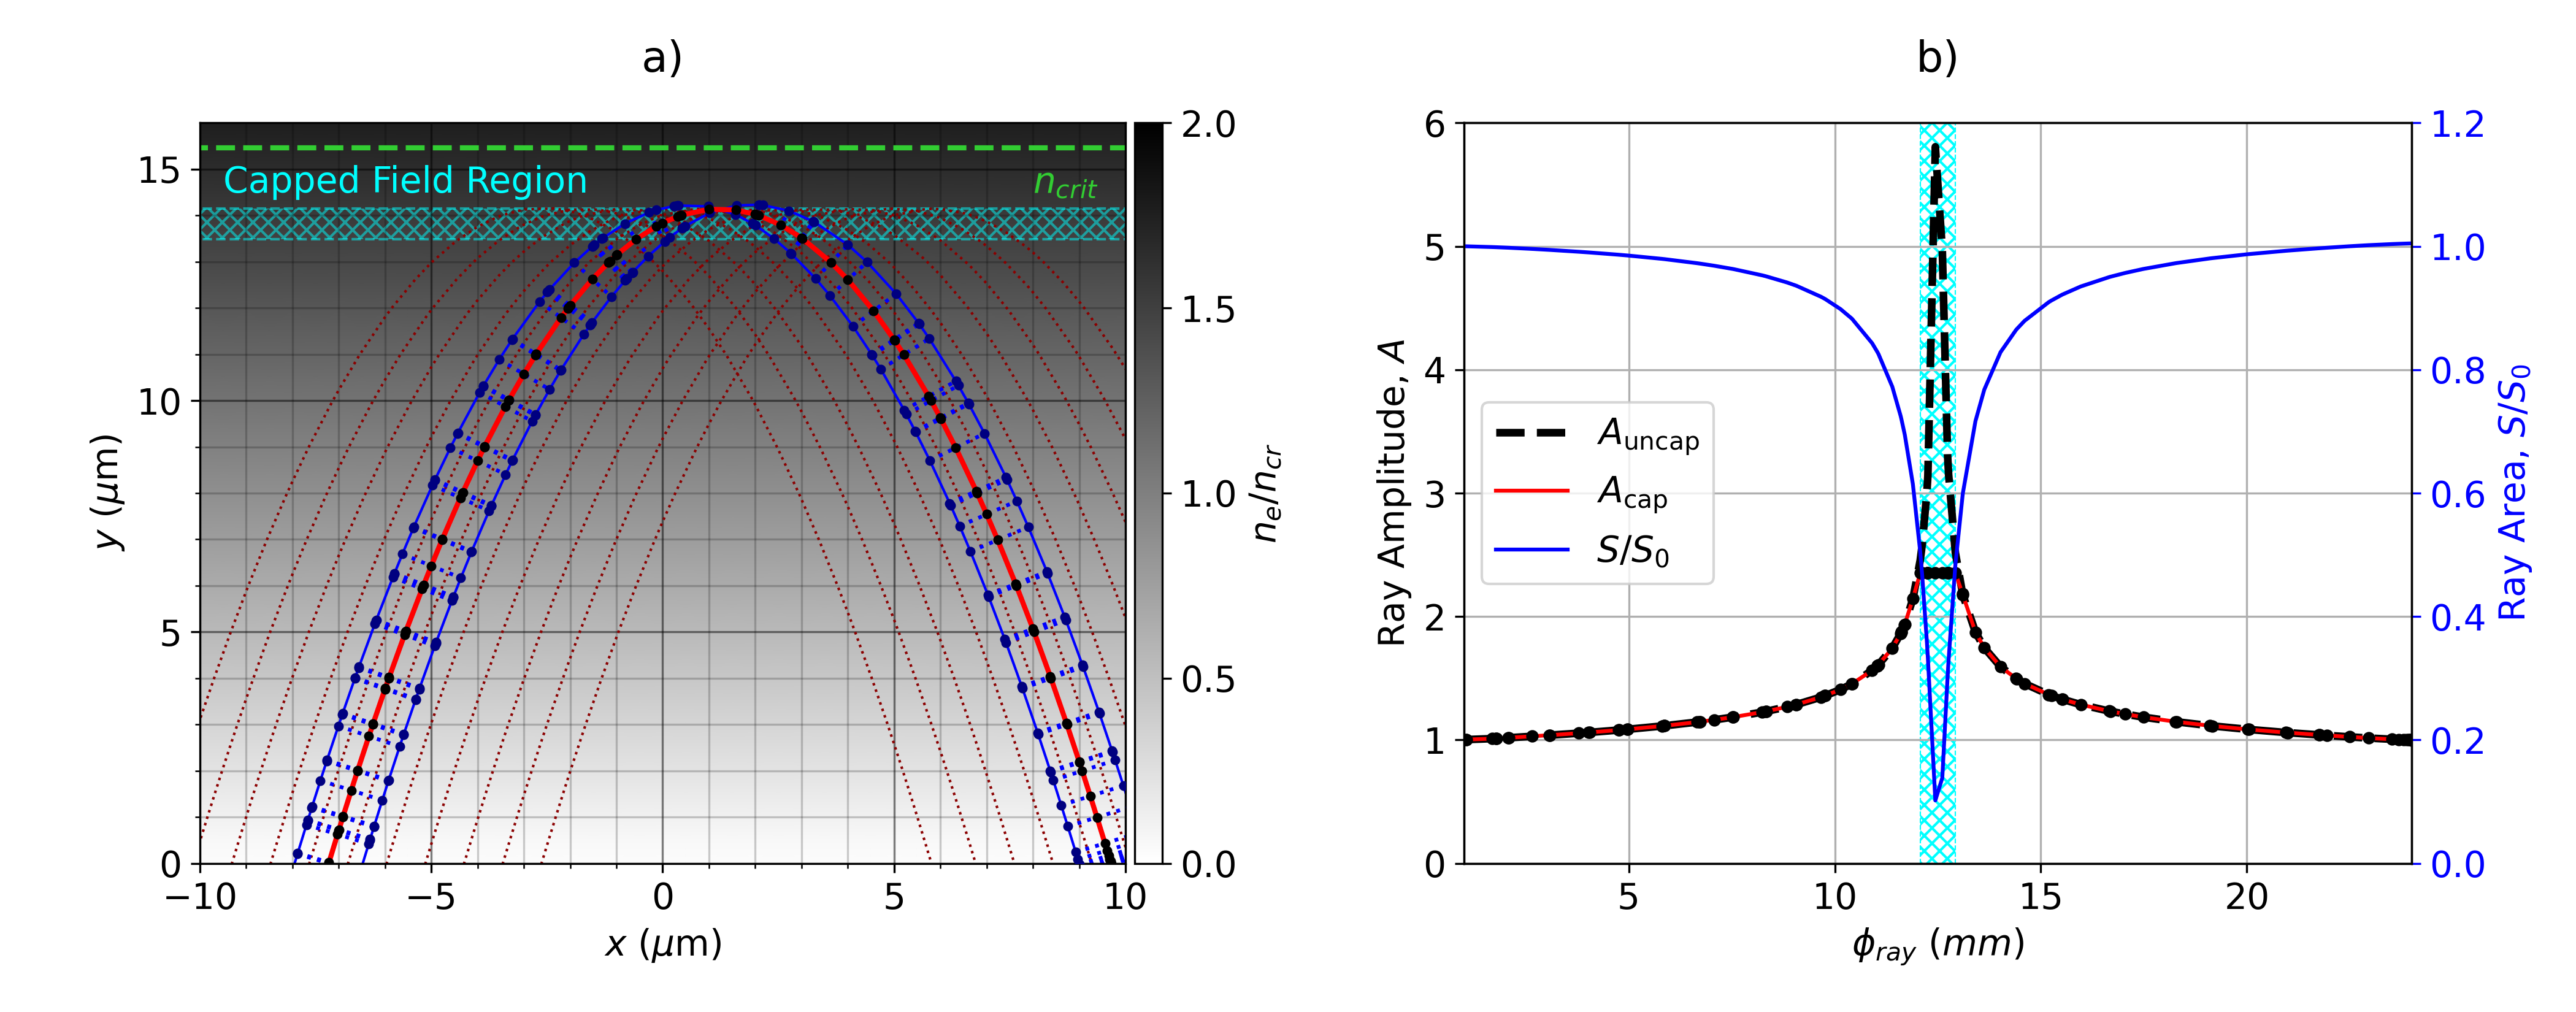
\includegraphics[width=\linewidth]{Numerics/Images/FieldCap_Diagram.png}
    \centering
    \caption{A demonstration of how the ray-amplitude is obtained from the area of neighbouring-rays for a beam propagating up a linear density gradient.
    Fig. a) explicitly shows the trajectory of a main-ray and its neighbour-rays in red and blue respectively, explicitly highlighting the beam's caustic region, where the amplitude of the light is capped.
    Fig. b) plots the area of the main-ray in blue (which goes through a minimum at the caustic location), as a function of the phase of the ray.
    Also shown are the uncapped and capped amplitudes of the ray.}%
    \label{fig:SOLAS_fieldcap_diagram}
\end{figure}

This method, which has been used successfully to model direct-drive \ac{CBET} in the \textsc{BeamCrosser} post-process code, is the approach taken to estimate the field in \textsc{Solas}.
Explicitly, for every ray that initialised for a \textsc{Solas} calculation, an additional 3 `neighbour-rays' are initialised in an equilateral triangle around it, perpendicular to the initial direction of propagation.
Note that when a 2-D ray-trace is used, only two neighbour-rays are required as the rays cannot change separation in the out of plane direction.
It is important to distinguish the dimension of the ray-trace, which is the number of dimensions in which rays can move in a simulation, to the dimension of the hydrodynamics.
For example, a 1-D spherical direct-drive \ac{Rad-Hydro} simulation still requires a 3-D ray-trace where rays can move in $x,\ y$ and $z$ for full accuracy.

These neighbour-rays are then co-traced up to the phase of the `main-ray' to evaluate the area of the main-ray on its phase front.
Fig.~\ref{fig:SOLAS_3draytube} plots an example of this co-tracing procedure for a single ray propagating in a 3-D direct-drive profile.
It can be seen that as the reflects away from the critical surface, the area diverges.
Note that artifically large neighbour-ray separation was used for this plot as it is purely illustrative.
Practically, the separation distance of the bundle of neighbour-rays (i.e. the side-length of the triangle, $\Delta l$) does not need to be infinitesimally small, but small enough that it accurately captures the local change of $|D(\tau)|$.
In terms of the hydrodynamic profiles, this means that $\Delta l \ll L_{n_e}$, where $L_{n_e}$ is the density length scale of the plasma.
For \textsc{Omega} scale direct-drive simulations, an initial separation of $\Delta l\lesssim 1\ \mu\text{m}$ is found to give converged behaviour.
If the separation is too small however, floating point arithmetic can lead to noise in the ray-amplitude estimation.
For all simulations presented in this thesis, $\Delta l=\lambda_0/10\ll1\ \mu\text{m}$ was used.

As mentioned in Sec.~\ref{sec:SOLAS_ray_propagation}, it was found that the Kaiser algorithm for ray propagation, which uses a single $\nabla n_e$ in each grid cell and discontinuously refracts rays at cell boundaries, led to large levels of noise in the ray-amplitude profiles.
In order to obtain smooth profiles for $A$, linear interpolation of $\nabla n_e$ was found to be necessary.
The continuously varying $\nabla n_e$, which does not have discontinuities across cell interfaces, allows a smoothly varying area for each ray to be obtained.

Fig.~\ref{fig:SOLAS_fieldcap_diagram}.a demonstrates this amplitude reconstruction process in a purely illustrative example of a beam travelling up a linear density gradient at an angle, leading to a caustic at its turning point.
The trajectory of several main-rays are plotted in dark-dashed red, and a single main-ray is highlighted in a brighter shade of red.
The two neighbour-rays of this highlighted main-ray are plotted in blue.
Note that in this figure, the default initial main-neighbour-ray separation of $\Delta l=\lambda_0/10=0.035\ \mu\text{m}$ was used, but the separation has been magnified on the plot to visualise the amplitude reconstruction from the area more clearly.
The locations of the main- and neighbour-rays after a single step of each main-ray are plotted as black and dark-blue spots respectively.
The `area' of the neighbour-rays $S$, which in this 2-D ray-trace example here is simply a distance, is plotted on~\ref{fig:SOLAS_fieldcap_diagram}.a as a dashed blue line between the neighbour-rays.
The neighbour-rays are pushed until they have the same phase as the main-ray, at which point the area is evaluated.

%##################################################
\subsubsection{Caustics and Ray-Sheets}%
\label{sec:SOLAS_caustics}

\begin{figure}[t!]
    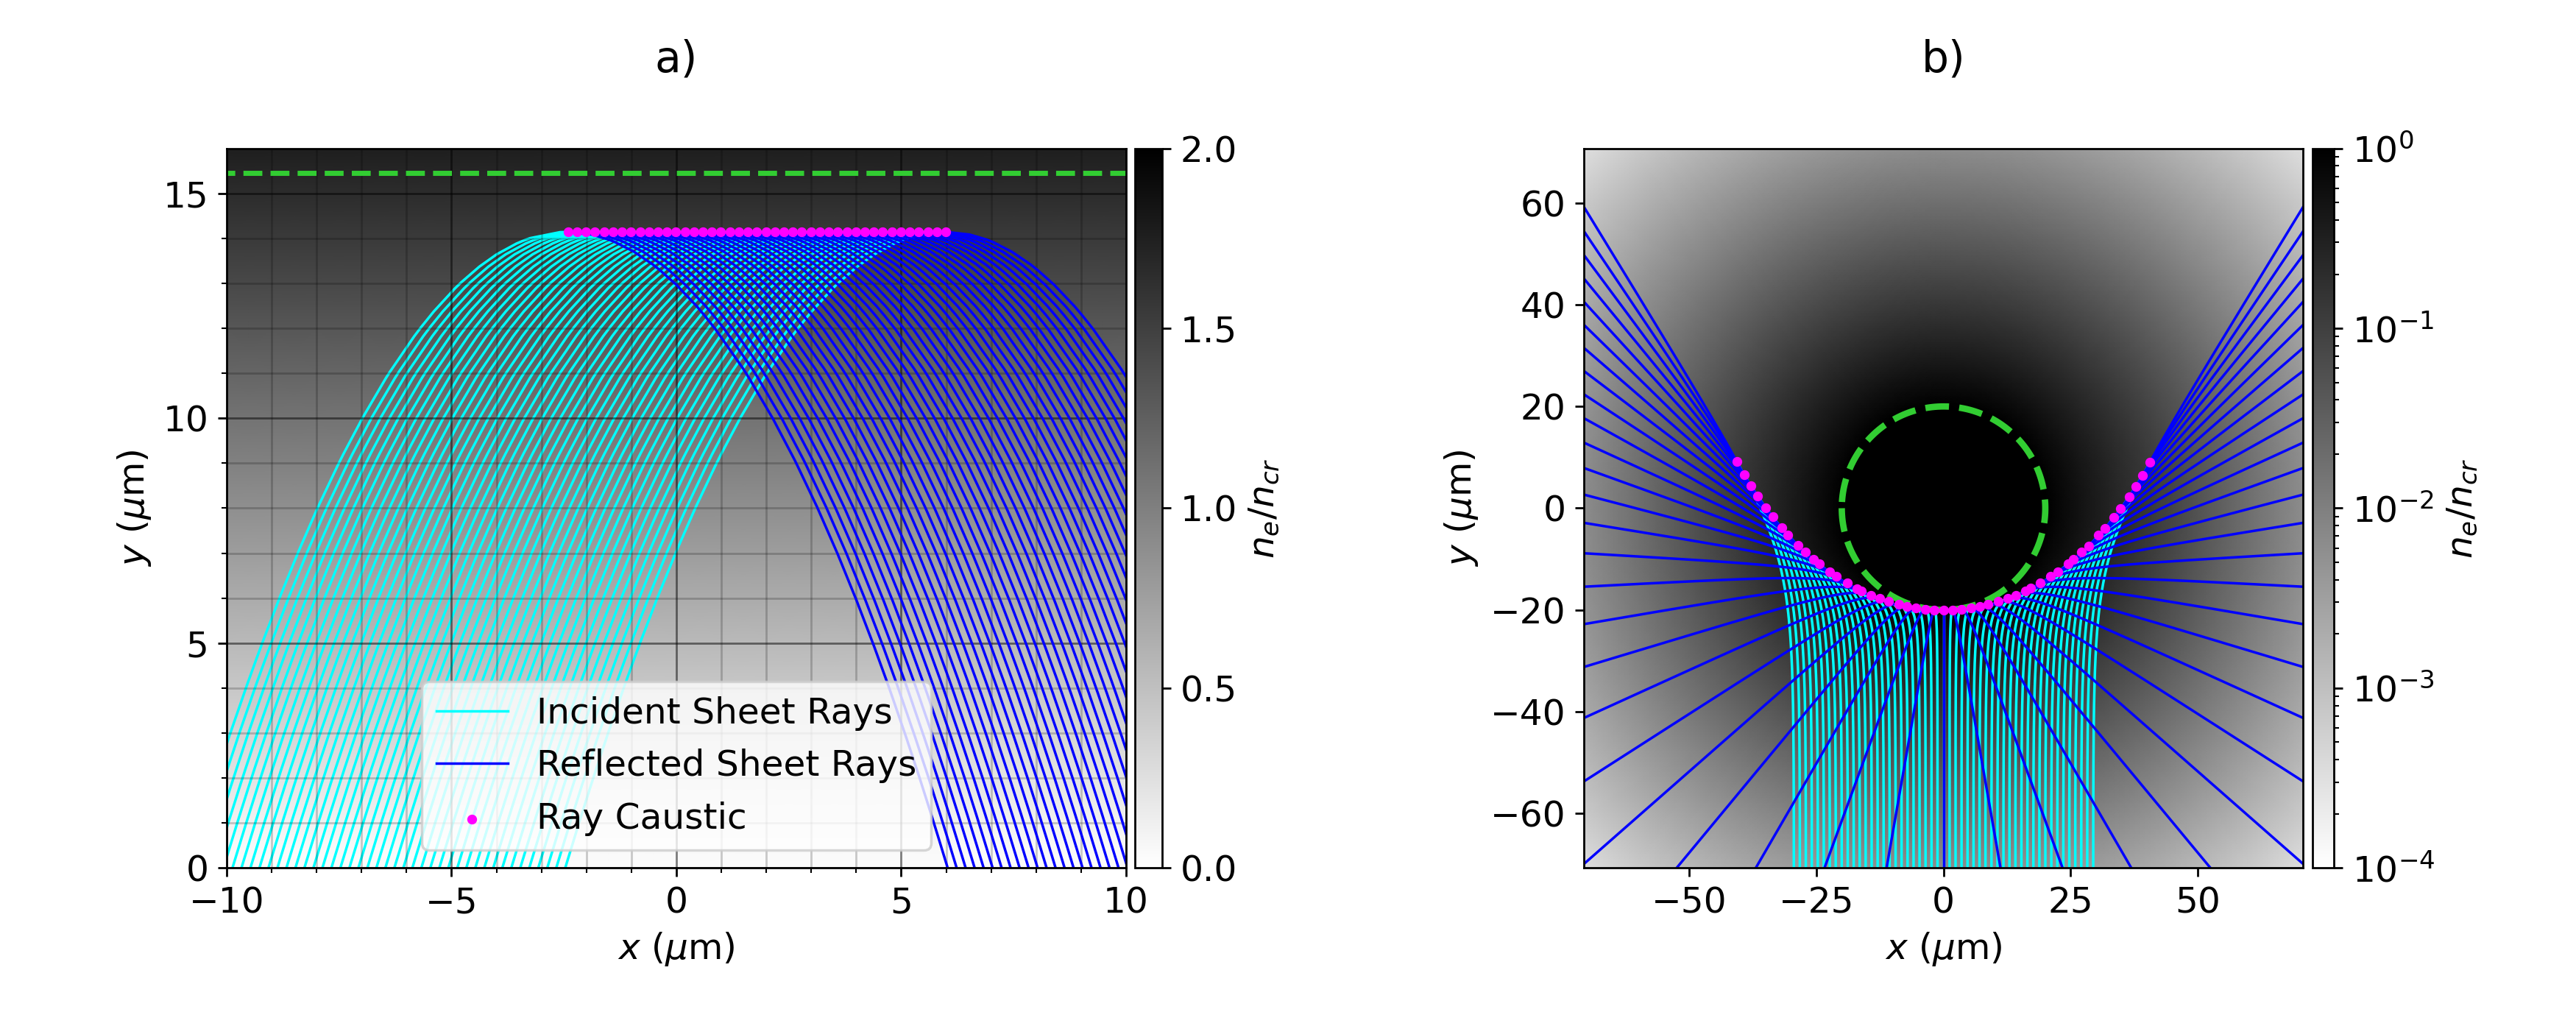
\includegraphics[width=\linewidth]{Numerics/Images/Raysheets_withcyl.png}
    \centering
    \caption{An illustration of the concept of caustics and ray sheets.
    In a), the trajectory of rays traversing up a linear density gradient are plotted.
    Separate colours are used for the incident and reflected sheets, which are separated by a caustic.
    In b), rays propagate up a density profile, $n_e=n_{\text{cr}}\exp{[ -(r_{\mu\text{m}}-20)/100 ]}$.
    Unlike in a), the ray caustics do not occur at their turning point, \textit{i.e.} the minimum radius.}%
    \label{fig:SOLAS_sheet_diagram}
\end{figure}

Caustics are an important concept in \ac{GO}, and the reconstructed field in their vicinity must be handled correctly in order to accurately model \ac{CBET} in ray-based codes.
Fig.~\ref{fig:SOLAS_fieldcap_diagram}.b plots the area of the main-ray as a function of main-ray phase in blue.
At $\varphi_{\text{ray}}\sim12\ \mu\text{m}$, $S\rightarrow 0$, \textit{i.e.} neighbouring-rays cross over each other, which is known as the ray-caustic.
In the absence of caustics, rays never cross over each other and therefore the mapping from ray phase-space (beam-port locations, where $\tau=0$) to real-space is single-valued, or in other words each point in space will be reached by (at most) one ray from each beam.
In the presence of caustics, this single-valued mapping breaks down and a single real-space location is accessible by multiple ray launch locations.
A single-valued mapping is still possible if each beam is separated into distinct `sheets' after caustics, where each sheet still has a single-valued projection from phase-space to real-space.

This is illustrated in Fig.~\ref{fig:SOLAS_sheet_diagram}.a, where rays from a single beam are plotted propagating up a linear density gradient with $n_e=n_{\text{cr}}y_{\mu\text{m}}/15.5$.
As the density gradient is purely in the $y$ direction, each ray has translational symmetry in $x$ and therefore each ray-caustic is located at the ray turning point, $y\sim14\ \mu\text{m}$.
The portions of the ray trajectories that fall before and after the caustic are separated into the `incident' and `reflected' sheets respectively and plotted in separate shades of blue.
Fig.~\ref{fig:SOLAS_sheet_diagram}.b also plots rays from a single beam, but now propagating through a cylindrically symmetric $n_e$ profile.
As can be seen from this figure, the caustic is not the same as the ray turning-point\footnote{Defined here as the location of maximal $n_e$ experienced along the ray trajectory.}, but it is the location that the amplitude diverges.

Unless the amplitude is tracked along each ray trajectory, the location of the caustic cannot be identified and rays cannot be separated into distinct sheets, both of which have important ramifications for ray-based \ac{CBET} models.
Firstly, because the amplitude diverges, the field values can become large and therefore must be capped to diffraction limited values (the \textsc{Solas} methods for this are discussed in more detail in Sec.~\ref{sec:SOLAS_caustic_cap}).
The power change of rays due to \ac{CBET} scales exponentially with field strength squared, so erroneously large field values are extremely problematic to accurately computing power changes.
Additionally, if the beam cannot be separated into distinct sheets, then self-\ac{CBET}, where the reflected component of a beam interacts with the incident component of the same beam, must be neglected.
In \textsc{Solas}, the neighbour-ray method allows the amplitude to be tracked along each ray, enabling caustic location identification and sheet-separation.
Currently, it is assumed that each sheet has two components, \textit{i.e.} an incident and reflected field, but it should be possible to extend this to multiple caustics to accurately model complex \ac{CBET} interactions such as target-stalk simulations~\cite{igumenshchev_effects_2009,igumenshchev_threedimensional_2016,gatujohnson_impact_2020}.
This is an advantage of the forward ray-tracing approach to \ac{CBET} modelling, compared to inverse-ray-tracing, where only plasma profiles that result in a single caustic can be modelled~\cite{colaitis_inverse_2021}.

The phase of the light is also evolved along each ray trajectory in equations~\ref{eq:SOLAS_rays}, and therefore the coherent sum of all electric fields can be reconstructed which involves interference between sheets.
The total electric field is,
\begin{equation}%
    \label{eq:SOLAS_Ecoherent}
    E = \sum_{j}^{\text{sheets}} |E_j|\exp{\left( i(k_0\varphi_j-\pi\alpha_j/2) \right)},
\end{equation}
where $k_0$ is the vacuum wavevector of the light and $\alpha_j$ accounts for the $\pi/2$ phase shift that occurs when a ray changes sheet, \textit{i.e.} $\alpha_j=0$ for the incident sheet and $\alpha_j=1$ for the reflected sheet \cite{follett_validation_2022}.

The fields are discretised on the \textsc{Solas} mesh by nearest neighbour interpolation from the ray to the cell.
When multiple rays from the same sheet pass through a cell, then the inverse-distance weighted average of the mid-point along the ray step to the cell centre is used to compute the field value for the cell.
This leads to a field structure, $|E_j|(\vec{x},\vec{k},\omega,\phi)$, where $j$ refers to each sheet, $\vec{x}$ is the spatial location of the field which refers to the cell the field is stored in, and $\vec{k},\omega,\phi$ are the wavevector, frequency and phase of the ray.
For many beam simulations, there is a large associated memory cost to store this information on the mesh, which is discussed in more detail in Sec.~\ref{sec:SOLAS_memory}.
When computing the effect of \ac{CBET}, it is also necessary to interpolate the fields stored at the cell centre to the ray trajectories.
Nearest neighbour interpolation is also used for this step, so rays experience a constant value for $|E_j|(\vec{x},\vec{k},\omega,\phi)$ throughout the cell.
It is technically possible to use higher order interpolation for both stages, either from an unstructured mesh of the ray locations, or from the \textsc{Solas} mesh, which is close to logically rectilinear.
The second of these options was tested but proved both to be the dominant computational cost for many beam \ac{CBET} interactions and also challenging to robustly implement for non-Cartesian meshes, because the angular resolution for typical spherical direct-drive simulations was too coarse for the required accuracy.

%################################################################################
%################################################################################
\subsection{Caustic Field Capping}%
\label{sec:SOLAS_caustic_cap}
In the vicinity of beam-caustics, the electric field magnitude of a beam is limited by diffraction which is neglected in \ac{GO}.
Therefore, ray-based models which do not cap fields near caustics can experience divergent electric fields.
For direct-drive simulations, a significant amount of \ac{CBET} occurs near caustics and therefore sensibly capping the field value is crucial for accurate simulations~\cite{colaitis_adaptive_2019}.
This cannot be achieved without knowledge of the caustic location, which is a severe limitation to the predictive capability of \ac{CBET} codes that do not track the amplitude.
This section describes two methods that have been implemented to cap the field values in the vicinity of laser caustics, the \ac{FL} and \ac{EI} approaches.

%##################################################
\paragraph*{Field Limiter}
This is a straightforward hard cap on the maximum value of the electric field reconstructed during the ray-trace.
The electric field of light propagating up a linear density gradient has the analytic solution of an Airy function.
The field limiter approach is to cap all electric fields to this value,
\begin{equation}
    \begin{gathered}
        \frac{|E|}{|E(\tau=0)|} = \sqrt{\frac{P(\tau)}{P(\tau=0)}} \min\left[ A, \sqrt{\zeta}\left( \frac{n_{\text{t}}}{n_{\text{cr}}} \right)^{1/4}, \sqrt{\zeta}\sqrt{\frac{S(\tau=0)}{S(\tau)}} \right], \\
        \zeta = 0.9\left( \omega L/c \right)^{1/3}, \\
        L = n_{\text{cr}}/|\nabla n_e|_\text{t},
    \end{gathered}
\end{equation}
where $n_{\text{t}}$ is the electron density at the caustic and $|\nabla n_e|_\text{t}$ is the magnitude of the electron density gradient at the caustic location~\cite{igumenshchev_crossedbeam_2012,follett_raybased_2018,kruer_physics_2003}.
The first term in the minimum is the standard field reconstruction from the amplitude away from caustics.
The second term is the maximum of the Airy function and the third term is an improvement to the second term for near-normally incident rays~\cite{follett_validation_2022}.
Fig.~\ref{fig:SOLAS_fieldcap_diagram}.b plots the uncapped and capped amplitudes obtained from the field limiter approach for light propagating at an angle to a linear density gradient.

%##################################################
\paragraph*{Etalon Integral}
The \ac{EI} method is an improvement to the \ac{FL}, which allows for deviations in the density profile away from linearity~\cite{colaitis_real_2019,kravcov_caustics_1999,kratsov_theory_2010}.
Several distinct types of caustic exist for different geometries of problem.
For example in direct-drive, the light reflecting from the critical surface forms a `fold'-type caustic, whereas focussing light leads to a more complex `cusp'-type caustic~\cite{lopez_metaplectic_2022}.
If the form of the caustic is assumed, then an approximation to the total field in the vicinity of the caustic is formulated, which allows for deviations from the ideal case.
In the example of the direct-drive fold caustic, the field is assumed to be the sum of an Airy function and its derivative, which accounts for the deviations from linearity.
An expression for the total field can be derived in terms of the ray-amplitude and phase before ($A_1$,$\varphi_1$) and after ($A_2$,$\varphi_2$) the caustic,
\begin{equation}
    \begin{gathered}
        E_T = \sqrt{\pi}\left[(-\xi)^{1/4}(A_1+A_2)\text{Ai}(\xi) - i(-\xi)^{1/4}(A_1-A_2)\text{Ai}'(\xi)  \right]e^{i(k_0\chi - \pi/4)}, \\
        \chi = \frac{1}{2}(\varphi_1+\varphi_2), \\
        \xi = -\left[ k_0\frac{3}{4}(\varphi_2-\varphi_1)  \right]^{2/3},
    \end{gathered}
\end{equation}
where $\text{Ai}$ and $\text{Ai}'$ are the Airy function and its derivative.
In \textsc{Solas}, $\text{Ai}$ and $\text{Ai}'$ are computed numerically using the \texttt{special-functions} library~\cite{chang_computation_1996}.
This total field can then be divided between the incident and reflected sheet by inversion of Eq.~\ref{eq:SOLAS_Ecoherent} assuming that $|E_1|=|E_2|$,
\begin{equation}
    \label{eq:SOLAS_etlon_int_field}
    \frac{\left|E_j\right|}{\left|E_{j, 0}\right|}=\frac{\sqrt{W_j}\left|E_T\right|}{\sqrt{2}\left[1+\sin \left(\varphi_2-\varphi_1\right)\right]^{1 / 2}}.
\end{equation}
The assumption of equal fields is approximately valid for \textsc{Omega} scale direct-drive conditions, where the caustic region is small compared to the plasma scales and therefore ray powers are assumed to not vary significantly over this distance.
The Etalon integral is applied in the `caustic-region', which in Refs.~\cite{asatryan_fresnel_1988,kravtsov_iv_1988,colaitis_real_2019}, is stated to be equivalent to,
\begin{equation}%
    \label{eq:SOLAS_causticregion}
    |\varphi_1-\varphi_2|\leq\lambda_0/2,
\end{equation}
where $\lambda_0$ is the vacuum wavelength of the light.

Applying the \ac{EI} method requires evaluation of Eq.~\ref{eq:SOLAS_causticregion} to determine if a ray is inside its caustic region, which relies on interpolation of the phase of the other sheet from the same beam onto the ray location.
If using nearest neighbour interpolation, such as in \textsc{Solas} for interpolation of all field quantities onto rays, a grid resolution of $\Delta\ll\lambda_0$ must be used, which is a much higher resolution than is required for ray-tracing and \ac{CBET} without the \ac{EI}.
Therefore, the \ac{EI} method is only used in \textsc{Solas} simulations for high resolution grid test problems, such as those Sec.~\ref{sec:SOLAS_field_validation}.
The alternative approach is to implement linear interpolation from the field quantities of all beams onto ray locations, such as in Ref.~\cite{follett_validation_2022}.
This was not deemed a viable approach however, because the mesh resolution for spherical simulations was found to not be well-enough angularly resolved to interpolate the phase with sufficient accuracy to the rays.
The standard procedure for \ac{CBET} simulations in \textsc{Solas} is to use the \ac{FL} approach, which was found to give satisfactory results compared to the \ac{EI} method.

%################################################################################
%################################################################################
\subsection{Field Reconstruction Validation}%
\label{sec:SOLAS_field_validation}

In this section, several test problems will be presented that compare electric fields obtained using the \textsc{Solas} field solver in the absence of \ac{CBET}, to those from the wave based solver \textsc{Lpse} in direct-drive relevant plasma profiles.
The \textsc{Lpse} results are presented in Ref.~\cite{follett_validation_2022}, and are available from the repository~\cite{follett_lpse_2022}.
In all the following test problems, the laser has a vacuum wavelength, $\lambda_0=0.351\ \mu\text{m}$ and a super-Gaussian intensity profile, defined in Eq.~\ref{eq:supgaus}.
All 1-D and 2-D validation problems assume lasers polarised out of the simulation plane along the $z$ axis.
The plasma density profiles are given by,
\begin{equation}%
    \label{eq:SOLAS_test_ne}
    n_e(r) = n_0 (d/r)^{m},
\end{equation}
where $n_0/n_{\text{cr}} = 1.165$, $d = 343\times S\ \mu\text{m}$, $m=3.78$ and $S$ changes the scale of the density profile, where $S=1$ corresponds to scale lengths from implosions using the full \textsc{Omega} laser-energy.
These values where obtained from fitting the equation to 1-D \ac{Rad-Hydro} calculations using the \textsc{Lilac} code.

%##################################################
\subsubsection{1-D Reflected Beam}

\begin{figure}[t!]
    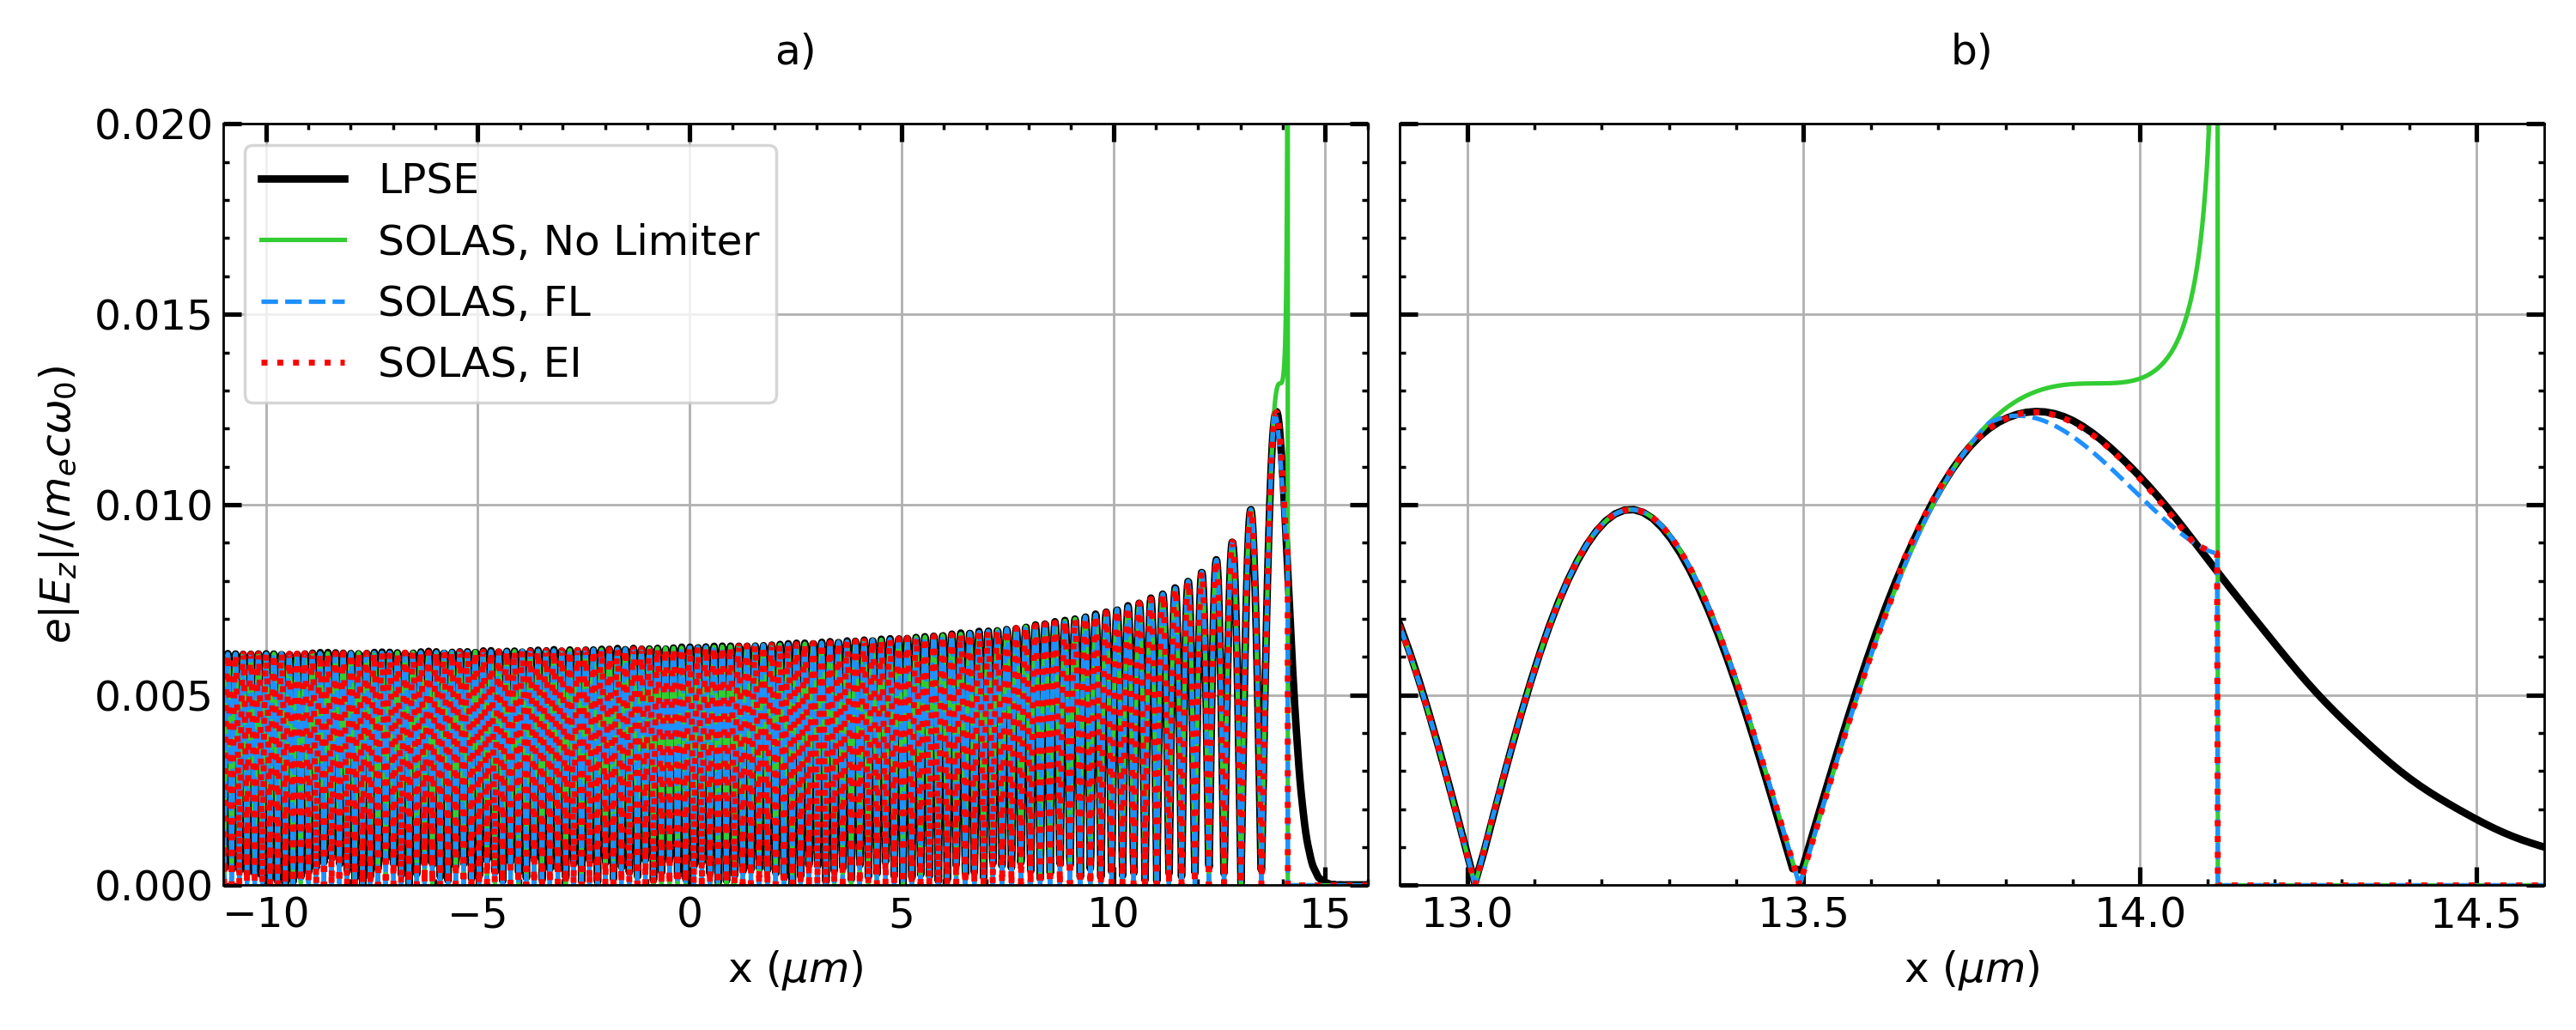
\includegraphics[width=\linewidth]{Numerics/Images/1d_field_capping.png}
    \centering
    \caption{Results of the 1-D field reconstruction test, comparing \textsc{Solas} fields with different caustic field capping methods to the \textsc{Lpse} results.
    Panel a) shows the oscillatory behaviour of the field solution which arises due to the interference between the incident and reflected sheet.
    Panel b) plots the same results, but zoomed in on the caustic region to demonstrate the differences in fields obtained from the different methods.}%
    \label{fig:SOLAS_1d_field_test}
\end{figure}

The first validation problem is for the case of light propagating normally up a density gradient.
For this problem, 1-D Cartesian geometry was used, so the density profile was obtained by transforming the spatial coordinate from equation~\ref{eq:SOLAS_test_ne}, $r\rightarrow x-36.42\ \mu\text{m}$.
The beam is travelled in the $+\hat{x}$ direction, with $I_0 = 14\ \text{W}/\text{cm}^{2}$.
Only a single ray was used because the ray-trace is completely 1-D.
A scale factor of $S=1/16$ was used, resulting in a critical surface at $x\sim 14.14\ \mu\text{m}$.
The simulation had bounds $x\in [-16,20]\ \mu\text{m}$ with a resolution of $\Delta x\sim 1\ \text{nm}$.
A high resolution was used here in order to resolve the highly oscillatory coherent field sum and also enabled use of the \ac{EI} field capping method.
Power changes of the rays due to \ac{Inv-Brem} and \ac{CBET} were also neglected.

The laser in this problem travelled up the density gradient, reflecting from the critical surface.
For light travelling normally up a density gradient, the critical density is the location of the caustic, because the ray area, $S(\tau)$, is constant and therefore the amplitude diverges when $\varepsilon\rightarrow 0$.
The total field is given by the coherent sum between the incident and reflected sheets.
Fig.~\ref{fig:SOLAS_1d_field_test}.a shows the \textsc{Lpse} result compared to the field obtained from \textsc{Solas} without a cap on the caustic field; using the \ac{FL} approach; and using the \ac{EI} approach.
The only difference between the \textsc{Solas} methods occurs in the caustic region\footnote{\textit{i.e.} where equation~\ref{eq:SOLAS_causticregion} is satisfied.}, shown more clearly in Fig.~\ref{fig:SOLAS_1d_field_test}.b, which in this problem is for $x>13.64\ \mu\text{m}$.
Failure to cap the caustic field leads to a divergent $|E_z|$ at the critical surface, but both the \ac{EI} and the \ac{FL} methods show good agreement with \textsc{Lpse}.
This justifies the default use of the simpler \ac{FL} method for \textsc{Solas} \ac{CBET} calculations.

Standard~\ac{GO} cannot capture the field beyond the critical surface because rays cannot propagate beyond $\varepsilon=0$.
The evanescent field in this region can be reproduced in the complex-\ac{GO} framework, which integrates rays which have complex-valued properties and can thus be evolved beyond the critical surface \cite{colaitis_real_2019}.
This, however, is not deemed to be necessary for accurate \ac{CBET} modelling of \textsc{Omega}-scale direct-drive implosions.

%##################################################
\subsubsection{2-D Reflected Beam}

\begin{figure}[t!]
    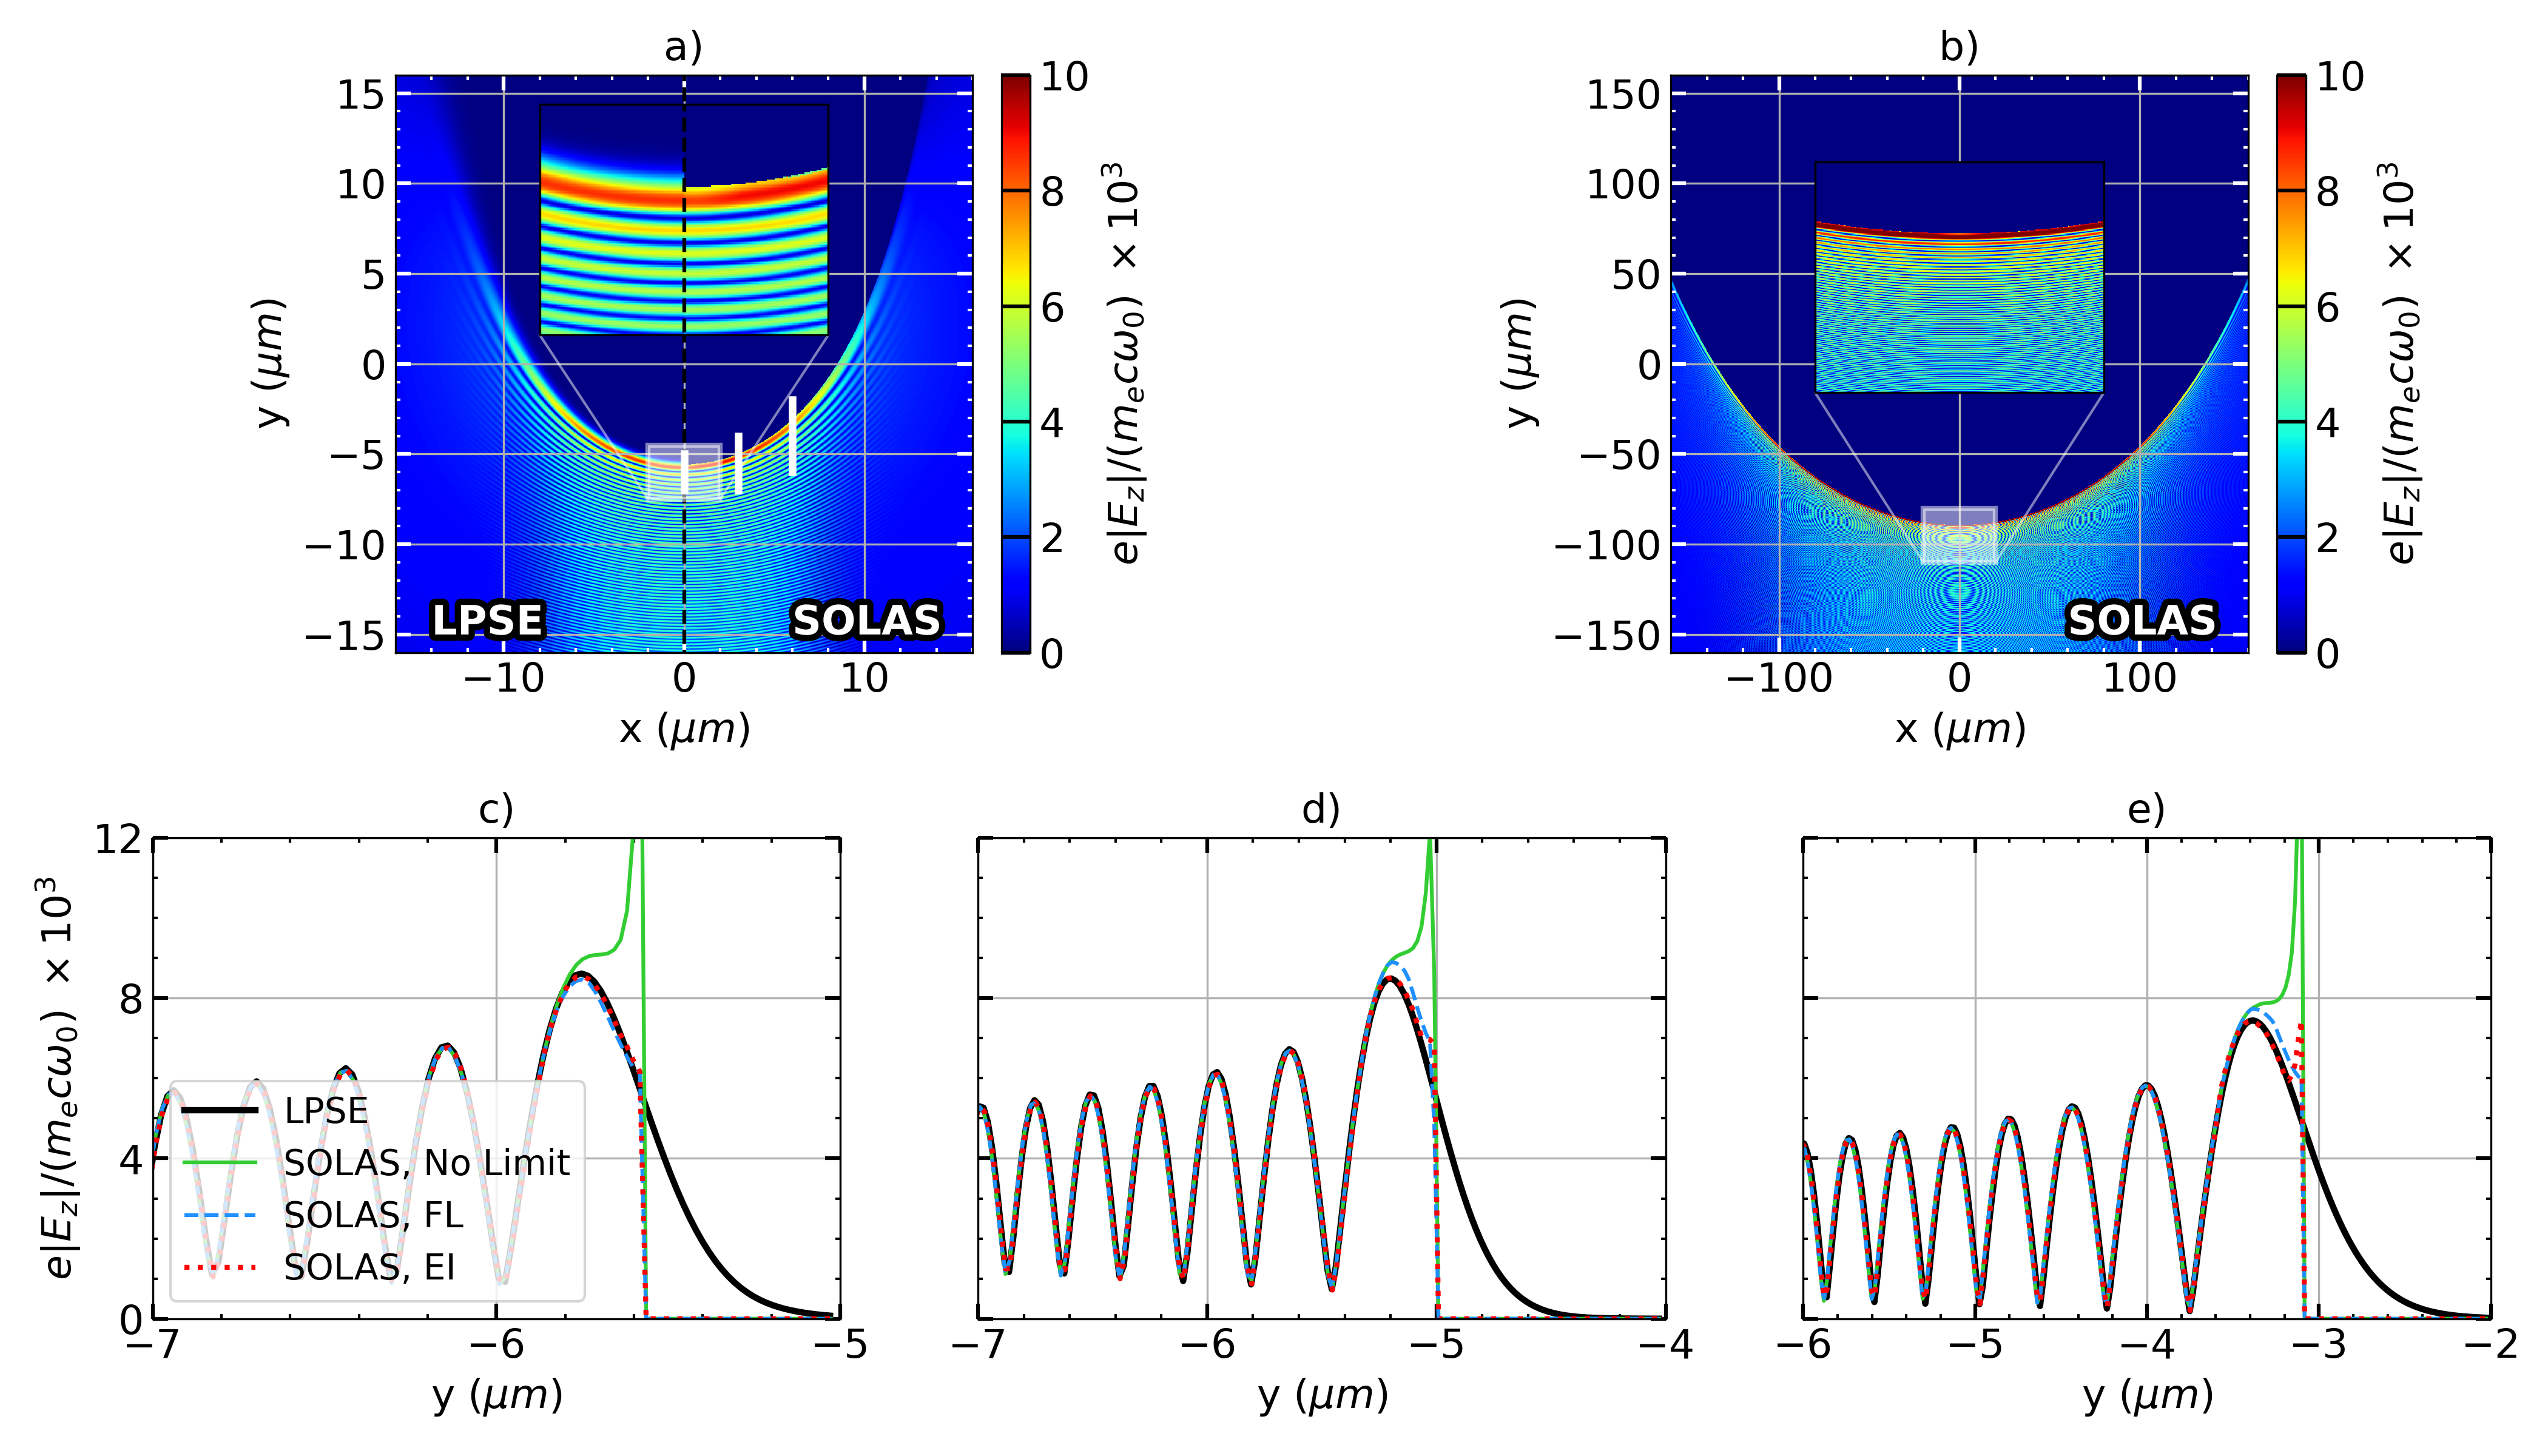
\includegraphics[width=1.0\linewidth]{Numerics/Images/2D_field_reconstruction_lineouts_alt.png}
    \centering
    \caption{Results of the 2-D field reconstruction test.
    Panel a) plots the field from \textsc{Lpse} on the left side and the \textsc{Solas} field on the right for the $1/64$ \textsc{Omega} scale simulation.
    Panel b) shows the \textsc{Solas} field from the $1/4$ scale simulation which, when compared to a), demonstrates that as scale increases, the relative size of the caustic region decreases.
    Panels c), d) and e) are lineouts near the caustic region along $y$ from the $1/64$ scale simulations at $x=0,\ 3$ and $6\ \mu\text{m}$ respectively, the positions of which are indicated by the white lines on a).
    Note that the circular features in the field in panels a) and b) arise due to aliasing artefacts between the true solution scale, with the resolution of the image and/ or simulation grid.}%
    \label{fig:SOLAS_2d_field_test}
\end{figure}

A second field reconstruction test was also implemented in 2-D geometry.
Unlike the previous 1-D test, the reconstructed field for this problem also depends on the divergence of neighbouring rays.
This is because apart from normally incident rays at the centre of the beam, $\vec{k}\nparallel\nabla n_e$, so the area, $S(\tau)$, of the rays vary.
Simulations at $1/64$ and $1/4$ scales are presented here.
The $S=1/64$ simulation bounds were $x,y\in [-20,20]\ \mu\text{m}$ and resolution $\Delta\ \sim 20\ \text{nm}$.
The $S=1/4$ simulation bounds were $x,y\in [-200,200]\ \mu\text{m}$ and resolution $\Delta\ \sim 100\ \text{nm}$.
For both scales, a single beam propagated parallel to $+\hat{y}$ and was centred on $x=0\ \mu\text{m}$.
The beam widths were $\sigma=8\ \text{and}\ 115\ \mu\text{m}$ for the $1/64$ and $1/4$ scales respectively.
The standard uniform sampling procedure described in Sec.~\ref{sec:SOLAS_ray_init} was used with $C_N=2$.
\ac{CBET} and \ac{Inv-Brem} were again both neglected.

Fig.~\ref{fig:SOLAS_2d_field_test}.a shows the \textsc{Lpse} and \textsc{Solas}, \ac{FL} fields for the $S=1/64$ setup.
Qualitative agreement is good between \textsc{Lpse} and the ray-based field in the sub-critical plasma.
The field from the \textsc{Solas} \ac{FL} $S=1/4$ simulation is plotted in Fig.~\ref{fig:SOLAS_2d_field_test}.b, from which it can be seen that the caustic region, which has a characteristic width $\sim\lambda_0$, shrinks in relative size as the scale increases.
This suggests that at increasing scale, the importance of accurate caustic modelling may decrease in importance.
Plotted in Figs.~\ref{fig:SOLAS_2d_field_test}.c,~\ref{fig:SOLAS_2d_field_test}.d and~\ref{fig:SOLAS_2d_field_test}.e are lineouts from the $1/64$ simulations taken at $x=0,\ 3\ \text{and}\ 6\ \mu\text{m}$ respectively.
They all include \textsc{Lpse} and \textsc{Solas} results with \ac{FL}, \ac{EI} caustic field capping along with no limiting.
These plots demonstrate that caustic field limiting is necessary to compare favourably to the \textsc{Lpse} solution and that the \ac{FL} approach slightly overestimates the caustic field compared to \textsc{Lpse} and the \ac{EI} method.
The discrepancy between the \ac{FL} and \ac{EI} results is again deemed sufficiently small to justify the default use of the simpler \ac{FL} approach.
To remind the reader, this choice is because the implementation of the \ac{EI} method in \textsc{Solas} requires grid resolution $\Delta\ll\lambda_0$, the reason for which is described at the end of Sec.~\ref{sec:SOLAS_caustic_cap}.

%###############################################################################################################################
%###############################################################################################################################
%###############################################################################################################################
\section{Ray-Based CBET Model}%
\label{sec:SOLAS_cbet_model}

\begin{figure}[t!]
    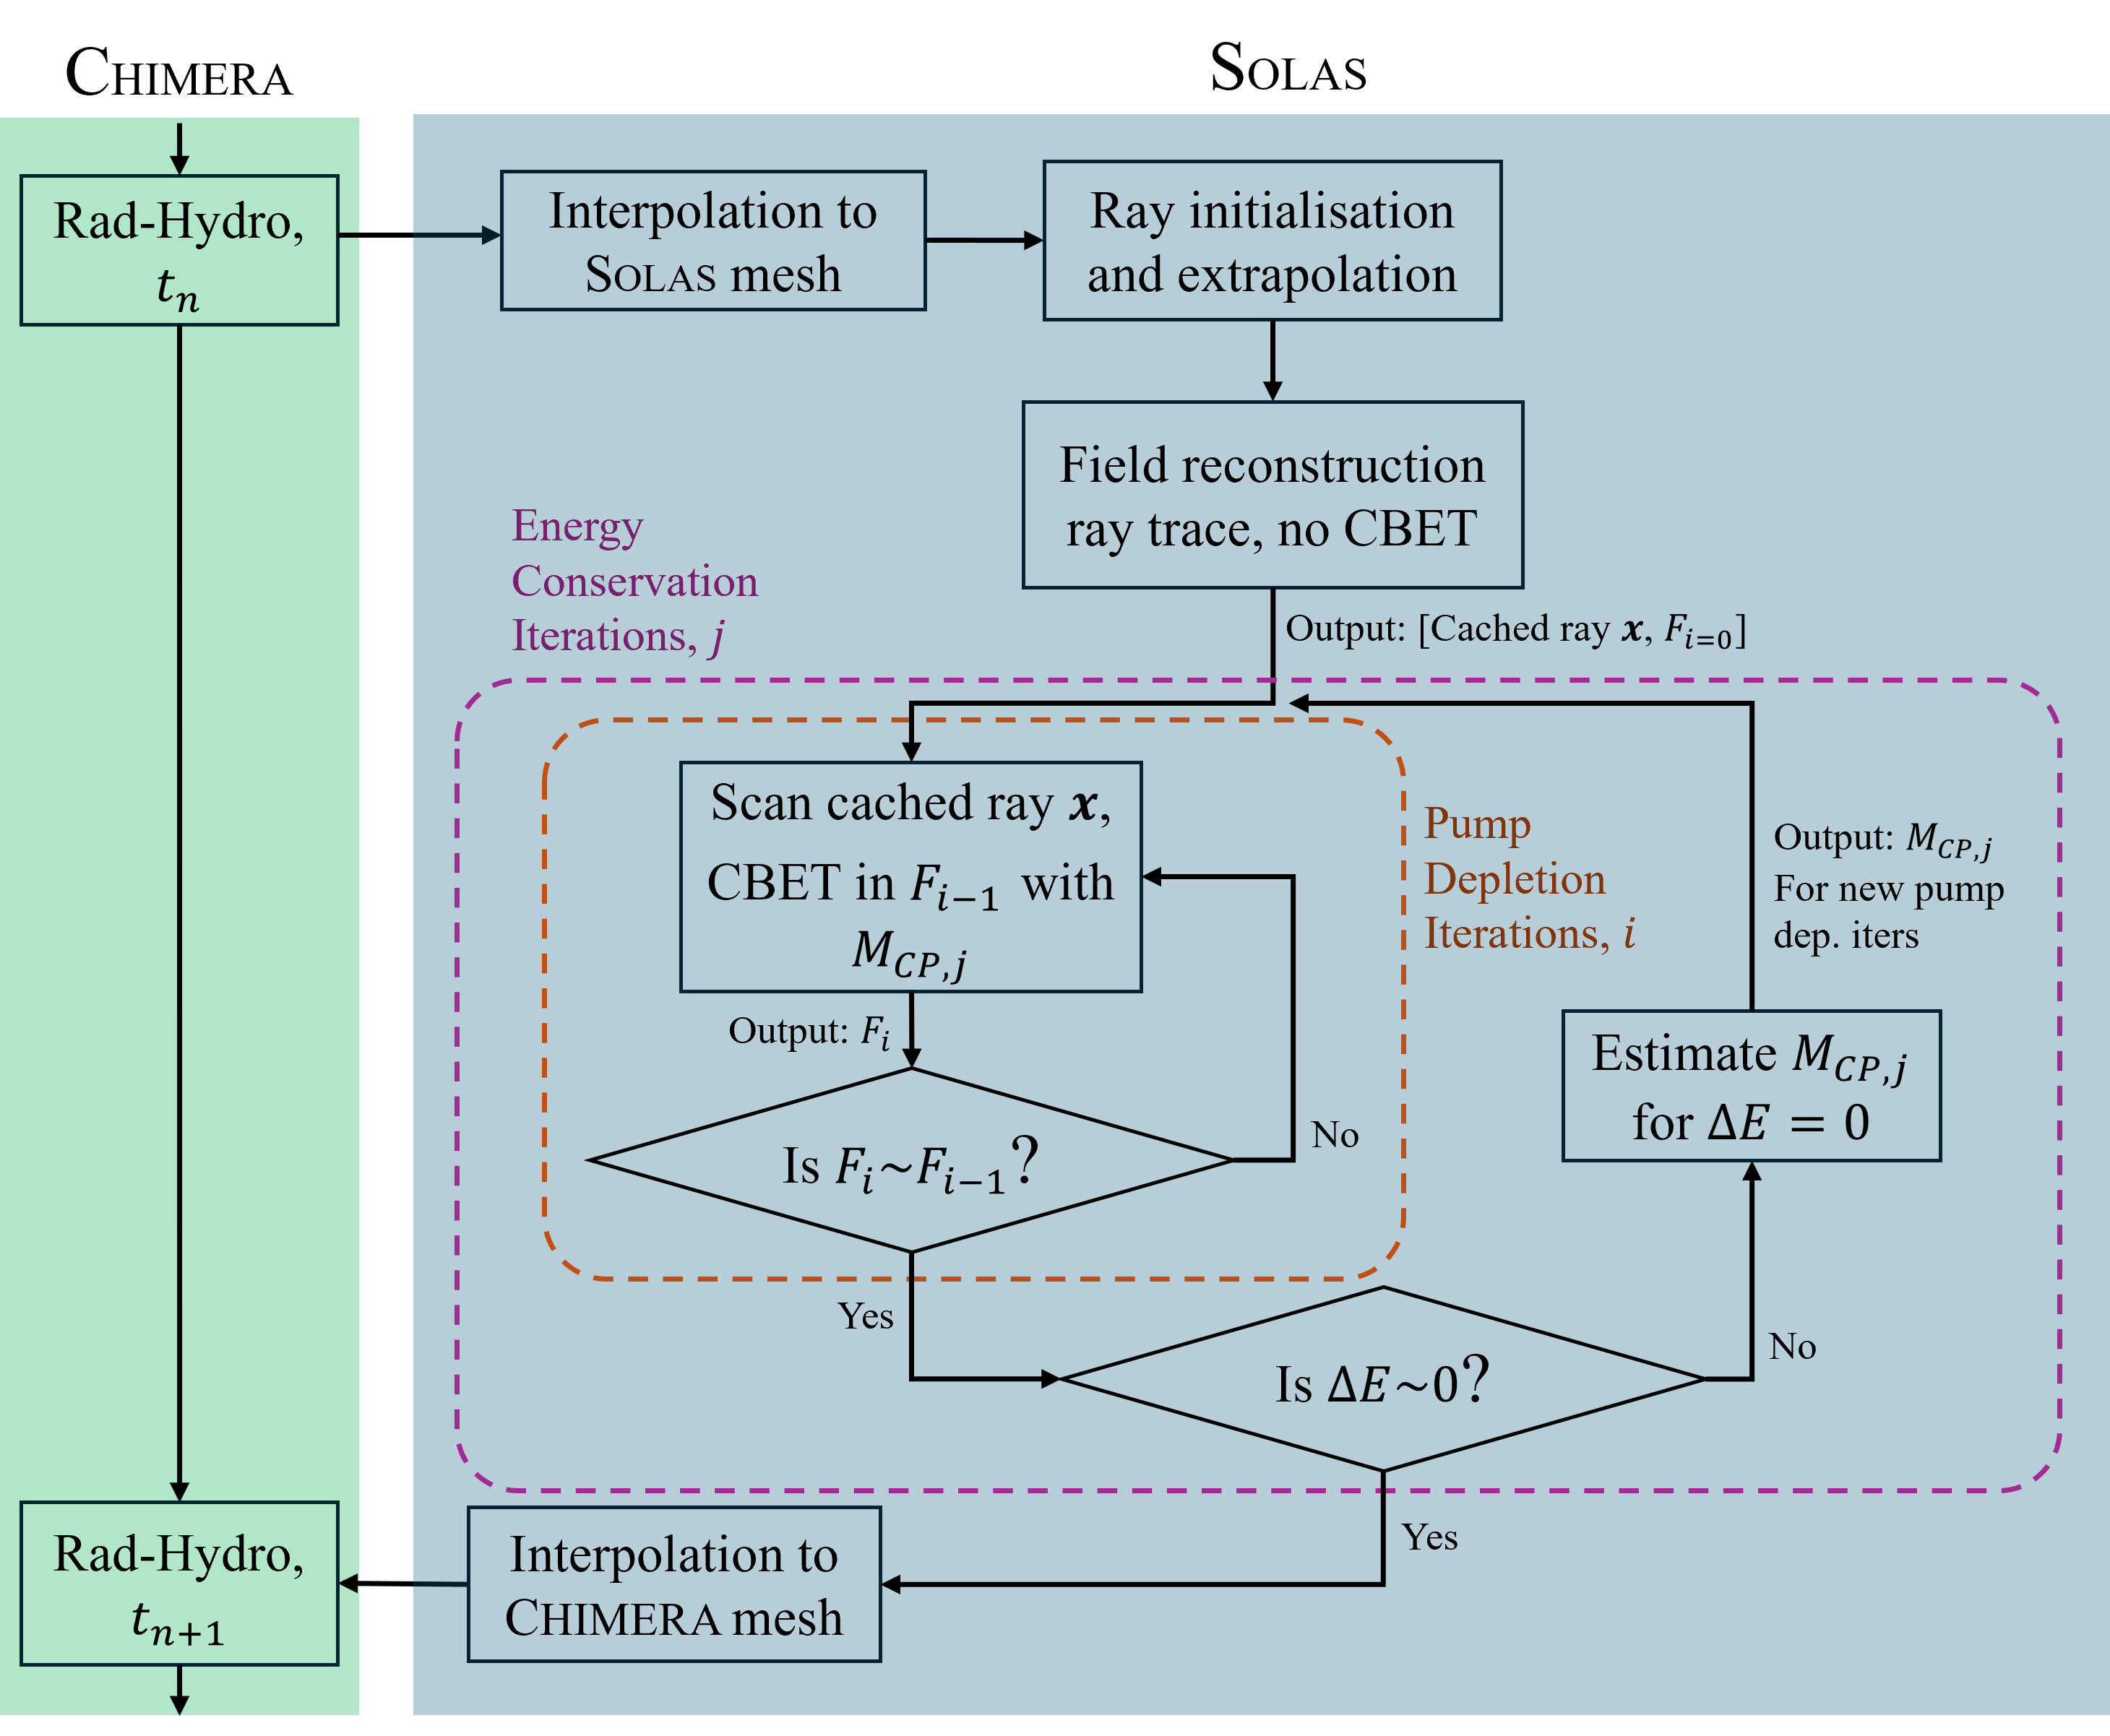
\includegraphics[width=0.9\linewidth]{Numerics/Images/CBET_flowchart.PNG}
    \centering
    \caption{The \textsc{Solas} \ac{CBET} model operation loop.
    $F_i$ is shorthand for the total field from all sheets at pump depletion iteration $i$ and $f_{\text{CP}}$ is the modifier to the caustic pump multiplier, described in Sec.~\ref{sec:energy_conserv_iters} of the $j^{\text{th}}$ energy conservation iteration.
    $\Delta E$ denotes the energy conservation error, which is the total incident power minus deposited power and power exiting the grid.}%
    \label{fig:SOLAS_CBET_flowchart}
\end{figure}

This section describes the implementation of the \ac{CBET} model in \textsc{Solas}.
Fig.~\ref{fig:SOLAS_CBET_flowchart} shows a flowchart which illustrates a broad overview of the operational loop of the \ac{CBET} model when coupled to \textsc{Chimera}.
The initial `field reconstruction' ray-trace in the absence of \ac{CBET}, follows the procedure described in Sec.~\ref{sec:SOLAS_field_reconstruc} to obtain the field for every sheet on the \textsc{Solas} mesh.
Ray-based \ac{CBET} models, including the model in \textsc{Solas}, typically must perform repeated ray-traces through the same hydrodynamic profiles to account for pump depletion and optionally energy conservation.

The pump depletion loop, described in more detail in Sec.~\ref{sec:pump_dep_iters}, is a fixed point iteration method to obtain the new \ac{CBET} laser fields.
This loop is necessary as each iteration produces a new background field which leads to a different \ac{CBET} interaction, which converges when \ac{CBET} has been fully accounted for.
The resultant solution will not necessarily conserve energy if \ac{CBET} occurs in the presence of laser caustics, due to errors in field reconstruction and \ac{CBET} scattering in these locations.
To remedy this, additional energy conservation iterations can be performed, where a multiplier on the \ac{CBET} gain in caustics can be varied to conserve laser energy.
Although this is an ad-hoc correction, it is found to lead to better agreement with higher fidelity solver, as is explicitly demonstrated in Sec.~\ref{sec:SOLAS_16beam_CBET}.

\ac{CBET} does not affect the trajectory of light, only its power and therefore repeating the calculations of ray trajectories is both computationally costly and unnecessary.
Ray locations are therefore stored in a memory-efficient, linked-list to be re-used in both loops.
It was found in \textsc{Solas} that caching the ray locations in this manner typically leads to an order of magnitude speed up compared to performing a new ray-trace for every iteration.

%################################################################################
%################################################################################
\subsection{Power Change of Rays due to CBET}%
\label{sec:SOLAS_ray_power_change}

Ray-tracing calculations assume steady-state hydrodynamic profiles for rays propagating through the plasma and that the field of a ray propagates as a plane wave along the ray path~\cite{ding_identify_2020}.
The linear gain theory of \ac{SBS}, which describes the steady-state energy change of locally plane wave light which passes through uniform plasma conditions, can therefore be used~\cite{randall_theory_1981,myatt_wavebased_2017}.
`Linear' in this context means that the plasma response to the driving fields is sufficiently small to be treated by a linear expansion.
The uniform assumption here means that the plasma conditions must not vary significantly over the interaction time or length scales.
For direct-drive conditions, hydrodynamic time scales are typically $\sim100 \text{ps}$ and \ac{CBET} saturates on the order of $\sim10 \text{ps}$.
Ray steps are also limited to grid cell boundaries, which are smaller than hydrodynamic length-scales, so it is safe to assume a locally uniform plasma background when this model is applied only over a single ray step at a time.

The steady-state interaction between two parallel-polarised sheets ($i,j$) over a path length $\text{d}\tau$ can be written in terms of the field magnitude of the sheet ($|E_{i,j}|$) or equivalently ray power ($P_{i,j} = A_{i,j}|E_{i,j}|^2$),
\begin{equation}
    \label{eq:SOLAS_CBET_power_change}
    \begin{gathered}
        \frac{\text{d}|E_i|^2}{\text{d}\tau}= \left( -\kappa_{\text{IB}} + \gamma_{ij} |E_j|^2 \right) |E_i|^2, \\
        \frac{\text{d}P_i}{\text{d}\tau}= \left( -\kappa_{\text{IB}} + \gamma_{ij} A_j P_j \right) P_i,
    \end{gathered}
\end{equation}
where $\kappa_{\text{IB}}$ is the \ac{Inv-Brem} absorption kernel, $A_j$ is the amplitude of sheet $j$ and $\gamma_{ij}$ is the \ac{CBET} gain of sheet $i$ from the interaction with sheet $j$.
The sheet/ ray which changes energy in a given interaction (here $i$), is often called the \textit{probe} while the other beam is termed the \textit{pump}.
The gain is a function of both the plasma conditions and the local field profiles for both sheets in the interaction, so a gain must be calculated between every pair of sheets at every location where both are present.
Going from the first to the second equation assumes that $\text{d}A_i/\text{d}\tau=0$, which is consistent with the assumption from the linear gain theory that the fields are approximately uniform over a small step.
Different models exist for the gain, which either use a fluid or kinetic treatment for the plasma \ac{IAW} response.

When multiple different probe beams are present, the total \ac{CBET} interaction is treated simply as the sum of all interactions from different sheets,
\begin{equation}
    \label{eq:SOLAS_CBET_power_change_allsheets}
    \frac{\text{d}P_i}{\text{d}\tau}= \left( -\kappa_{\text{IB}} + \kappa_{\text{CBET}} \right) P_i,
\end{equation}
where the \ac{CBET} kernel has been defined $\kappa_{\text{CBET}} = \sum_{j\neq i} \gamma_{ij} |E_j|^2$.
This summation assumes that the fields from different sheets are uncorrelated.
For direct-drive conditions, this assumption is broadly correct, apart from when a probe sheet undergoes a \ac{CBET} interaction in the caustic region of the probe.
In this case, the \textit{Coherent Caustic} correction is applied, which is described in Sec.~\ref{sec:SOLAS_coherent_caustic}.

Note that when computing both \ac{Inv-Brem} and \ac{CBET}, the partition of power lost to each interaction can be computed as,
\begin{equation}
    \label{eq:CBET_deposition}
    \begin{gathered}
        \Delta P_{i,\text{IB}} = - \langle P_i\rangle \frac{\kappa_{\text{IB}}}{\kappa_{\text{CBET}} - \kappa_{\text{IB}}}, \\
        \Delta P_{i,\text{CBET}} = \langle P_i\rangle \frac{\kappa_{\text{CBET}}}{\kappa_{\text{CBET}} - \kappa_{\text{IB}}}, \\
        \langle P_i\rangle = P_i  + P_i\left( \kappa_{\text{CBET}} - \kappa_{\text{IB}} \right)\text{d}\tau/2,
    \end{gathered}
\end{equation}
where $\Delta P_{i,\text{IB}}$ and $\Delta P_{i,\text{CBET}}$ are the powers lost to \ac{Inv-Brem} and \ac{CBET} respectively and $\langle P_i\rangle$ is the average power of the ray over the step, $\text{d}\tau$.
This can be derived by solving Eq.~\ref{eq:SOLAS_CBET_power_change} for $P_i$ and then taking the limit $\text{d}\tau\rightarrow0$ \cite{marozas_wavelengthdetuning_2018}.
The deposition, $\Delta P_{i,\text{IB}}$, can then be interpolated to the grid as an electron energy source as is described in Sec.~\ref{sec:SOLAS_ray_propagation}.

The two formulations of the gain are presented below.
Broadly, the gain describes the plasma response to the 2 driving fields and therefore dictates the energy transfer between them.
They differ in that the fluid formulation arises by deriving a gain from linearised fluid equations for the plasma response, whereas the kinetic formulation is obtained from a linearisation of the Vlasov equation.
The kinetic gain is more complete and should be used for comparison to experimental observables, whereas the fluid gain is useful for comparison with \textsc{Lpse}, which directly solves the linearised fluid equations.

%##################################################
\paragraph*{Fluid CBET Gain}

The linear fluid gain, derived by Randall \textit{et al.} in Ref.~\cite{randall_theory_1981} is,
\begin{equation}
    \label{eq:SOLAS_CBET_fluid_gain}
    \begin{gathered}
        \gamma_{ij} = \frac{n_e e}{4 m_e c \omega_i} \frac{1}{T_e \left( 1 + 3 T_i / Z T_e \right)} \frac{R(\eta_{ij})}{\nu_{\text{ia}}}, \\
        R(\eta_{ij}) = \frac{ (\nu_{\text{ia}}/\omega_{s})^2 \eta_{ij} } { (\eta^2 - 1)^2 + (\nu_{\text{ia}}/\omega_s)^2 \eta_{ij}^2 }, \\
        \eta_{ij} = \frac{ (\omega_j-\omega_i) - \vec{k}_s.\vec{u} }{\omega_s},
    \end{gathered}
\end{equation}
where $T_e$ and $T_i$ are the electron and ion temperatures in $\text{eV}$ respectively, $\omega_i$ and $\vec{k}_i$ are the frequency and wavevector of sheet $i$ respectively, $Z$ is the ionisation state, $\vec{u}$ is the fluid velocity, $\omega_s = |\vec{k}_s|c_s$ is the \ac{IAW} frequency, $\vec{k}_s = \vec{k}_j - \vec{k}_i$ is the \ac{IAW} wavevector, $c_s = \sqrt{e(Z T_e + 3 T_i)/m_i}$ is the sound speed and $\nu_{\text{ia}}$ is the \ac{IAW} damping rate.
This formulation is useful for comparison with \textsc{Lpse}, which directly solves the linearised fluid equations and therefore in situations where the \ac{GO} assumptions are valid, the two methods should give similar results.
However, it is generally not considered to be a good choice of model to compare to experiment.
The damping rate, $\nu_{\text{ia}}$ does not have an analytic formula for arbitrary plasma conditions and therefore must be prescribed.
Additionally, Eq.~\ref{eq:SOLAS_CBET_fluid_gain} assumes an average ion treatment of the species in the plasma if multiple ion species are present.
In reality, both fast and slow modes of \ac{IAW} can be driven in a 2-species plasma~\cite{williams_frequency_1995}, which can independently lead to \ac{CBET} scattering.
This effect cannot be captured using the fluid gain, where the plasma is assumed to made of a single ion species with a number density averaged ion mass.
Codes that use this formulation typically use a damping value $\nu_{\text{ia}}/\omega_s=0.2$ for CH plasmas, which is the value used for all fluid gain simulations in this chapter.

%##################################################
\paragraph*{Kinetic CBET Gain}

The linear kinetic \ac{CBET} gain, described by Michel in Ref.~\cite{michel_saturation_2013} is,
\begin{equation}
    \label{eq:SOLAS_CBET_kinetc_gain}
    \begin{gathered}
        \gamma_{ij} = \frac{e^2 |\vec{k}_s|^2}{4 m_e^2 c \omega_i^3}\text{Im}(K_{ij}), \\
        K_{ij} = \frac{\chi_e(1+\chi_i)}{(1+\chi_e+\chi_i)}, \\
        \chi_e = \frac{-1}{2 |\vec{k}_s|^2 \lambda_{De}^2} \text{Z}'\left( \frac{(\omega_j-\omega_i)-\vec{k}_s.\vec{u}}{\sqrt{2} |\vec{k}|_s v_{Te}} \right), \\
        \chi_i = \frac{-1}{2 |\vec{k}_s|^2 \lambda_{De}^2} \frac{T_e}{\langle Z\rangle T_i} \nsum_{\alpha}^{\text{species}} f_{\alpha}Z_{\alpha}^2  \text{Z}'\left( \frac{(\omega_j-\omega_i)-\vec{k}_s.\vec{u}}{\sqrt{2} |\vec{k}|_s v_{T\alpha}} \right), \\
    \end{gathered}
\end{equation}
where $\chi_e$ and $\chi_i$ are the electron and ion susceptibilities respectively, $f_{\alpha}$ and $Z_{\alpha}$ are the number fraction and ionisation of ion species $\alpha$ respectively, $\text{Z}'$ is the derivative of the plasma dispersion function, $v_{Tn}=\sqrt{e T_n/m_n}$ is the thermal velocity of species $n$ with temperature $T_n$ in eV and mass $m_n$, $\lambda_{De}=\sqrt{\varepsilon_0 e T_e / n_e e^2}$ is the electron Debye length and $\langle Z \rangle = \sum_{\alpha}f_{\alpha}Z_{\alpha}$ is the average ionisation.
Note that the susceptibilities $\chi_{i,e}$ are complex.
In order to compute $\text{Z}'$ in \textsc{Solas}, the \texttt{CALGO} library is used to numerically compute the value of the \textit{Fadeeva function}, $w(x)$~\cite{poppe_algorithm_1990}.
This is then related to the plasma dispersion function and its derivative by,
\begin{equation}
    \label{eq:SOLAS_plasma_disp_func}
    \begin{gathered}
        \text{Z}(x) = i\sqrt{\pi} w(x), \\
        \text{Z}'(x) = -2 [1 + x \text{Z}(x)],
    \end{gathered}
\end{equation}
where $i=\sqrt{-1}$ and $w(x)$, $\text{Z}(x)$ and $\text{Z}'(x)$ are all complex numbers~\cite{fried_plasma_1961}.
Unlike the fluid gain, this theory correctly captures the resonance and has no effective free parameters, making it the judicious choice for predictive simulations.
The plasma dispersion function is however relatively slow to numerically evaluate and dominates computational runtime if evaluated every ray step.
\textsc{Solas} therefore calculates $\gamma_{ij}$ between each sheet in every grid cell at the end of the field reconstruction ray-trace (from Fig.~\ref{fig:SOLAS_CBET_flowchart}) and then interpolates this pre-calculated value onto the ray locations for the pump-depletion iterations.
This reduces computational runtimes by orders of magnitude for many beam direct-drive simulations, but has an associated memory overhead, which is discussed in more detail in Sec.~\ref{sec:SOLAS_memory}.
All simulations in this thesis use the kinetic \ac{CBET} gain unless explicitly stated otherwise.

%##################################################
\paragraph*{Random Polarisation Correction}

The gains calculated above all assume that the interacting fields have parallel polarisations.
For many laser systems, beams may have arbitrary or random polarisations, such as at the \textsc{Omega} laser facility where \ac{DPRs} separate each beam into 2 orthogonally polarised sub-beams which overlap to effectively have one spot with random polarisation \cite{boehly_reduction_1999}.
If a simulation is conducted with multiple beams of random polarisation, a \textit{Polarisation Smoothing} multiplier, $M_{\text{PS}}$, must be applied to the value of $\gamma_{12}$ which accounts for random polarisation angles between the field from different sheets,
\begin{equation}
    \label{eq:polarisation_smoothing}
    M_{\text{PS}} = \frac{1}{4}(1 + \cos^2\theta),
\end{equation}
where $\theta$ is the angle between the wavevectors of the interacting sheets.

%################################################################################
%################################################################################
\subsection{Caustic Gain Truncation}%
\label{sec:SOLAS_caustic_gain_truncation}

\begin{figure}[t!]
    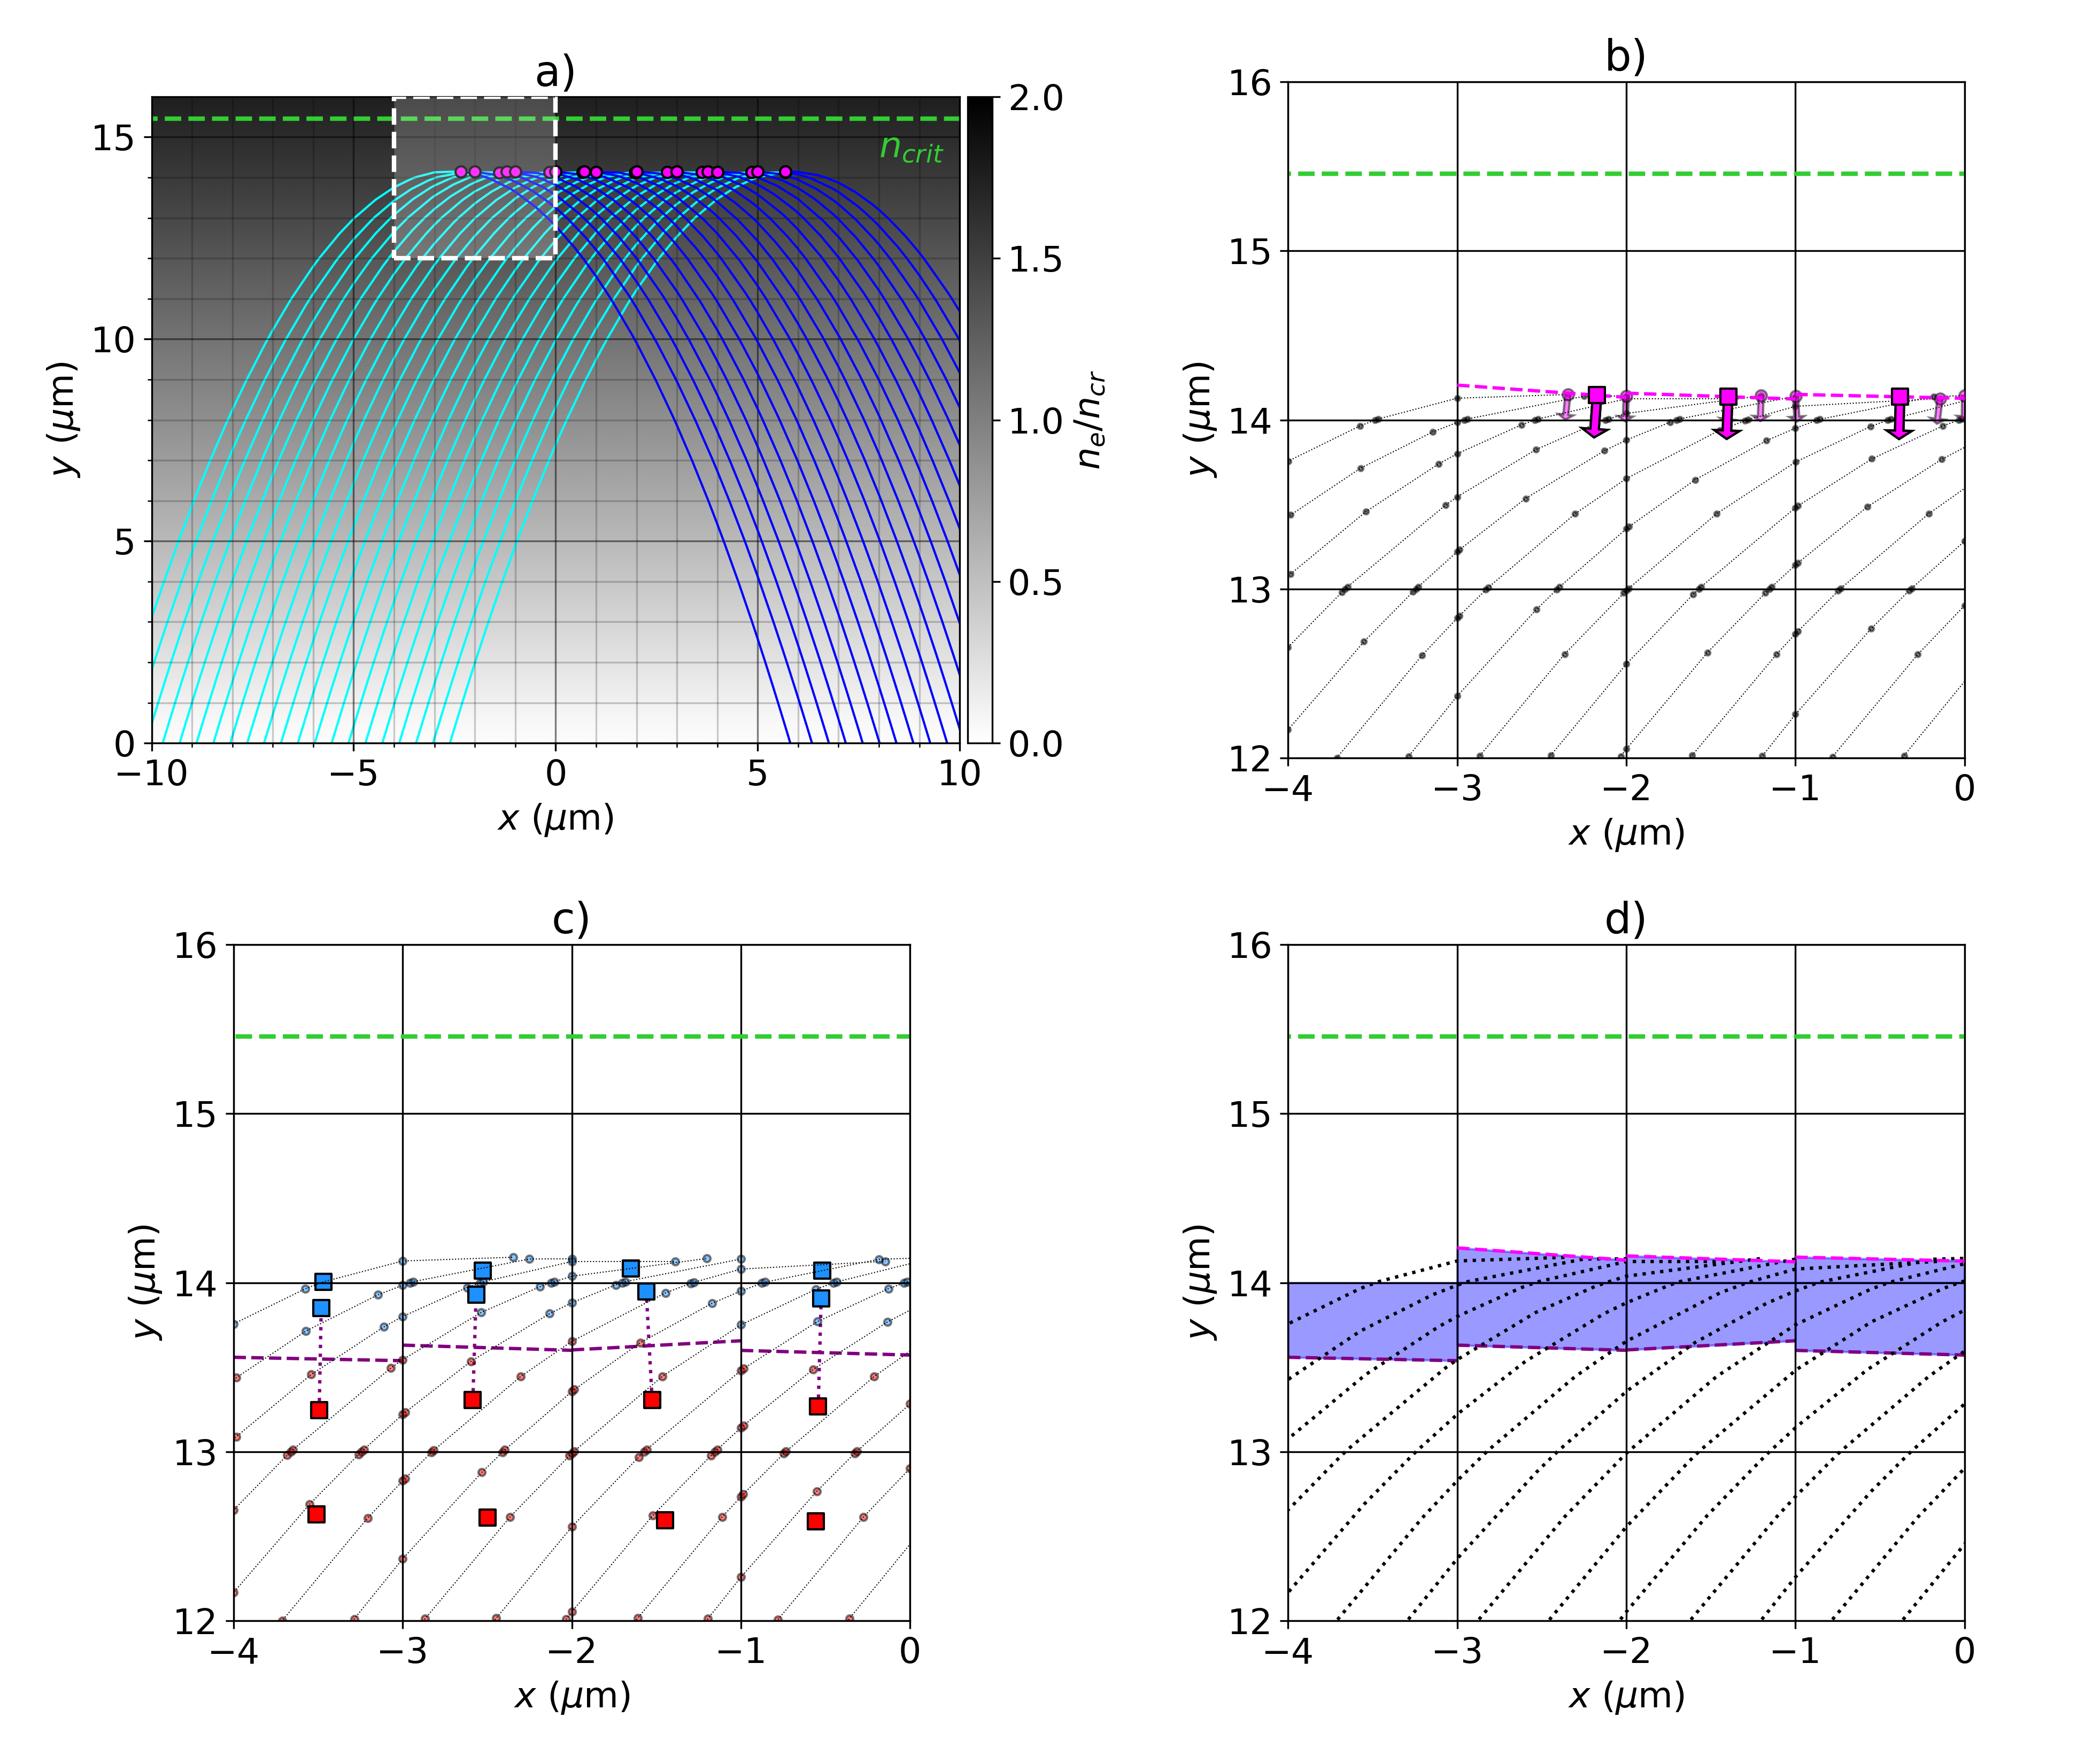
\includegraphics[width=1.0\linewidth]{Numerics/Images/caustic_region_diagram.png}
    \centering
    \caption{Illustration of the \ac{CGT} and caustic region identification algorithms.
    Panel a) shows a laser, separated into incident and reflected sheets by a caustic, propagating up and reflecting in a linear density ramp.
    \ac{CGT} is illustrated in b) where a cell is separated into a \textit{lit} and \textit{unlit} region by the reconstructed \textit{caustic plane} (dashed magenta line).
    Panels c) and d) illustrate the method used to identify the \textit{caustic region} (shaded blue), where the coherent caustic modifier is applied.
    c) shows that cells are geometrically separated into \textit{capped} (blue squares) and \textit{uncapped} (red squares) regions and the coherent caustic modifier to the gain is applied in this capped, caustic-region.}%
    \label{fig:SOLAS_caustic_region}
\end{figure}

For rays propagating through \textsc{Solas} cells, nearest neighbour interpolation is used to interpolate field quantities to the rays.
This is generally an adequate approximation for field magnitudes, frequencies and wavevectors, which vary over greater length scales than typical cell resolutions $\mathcal{O}(1 \mu\text{m})$, apart from in the vicinity of a caustic \cite{follett_validation_2022}.
Near caustics, rays turn sharply and fields have a sharp cut-off, dropping to zero sharply, as be seen in the lineouts from Fig.~\ref{fig:SOLAS_2d_field_test}.
The sharp turning of rays mean that $\vec{k}$ can vary rapidly within a cell.
Although \textsc{Solas} does have variable radial resolution, as described in Sec.~\ref{fig:SOLAS_combined_cells}, this resolution is limited to the minimum radial cell size from the hydrodynamic grid, which is not dictated from laser parameters and cells are typically larger than the caustic region width $\mathcal{O}(\lambda_0)$.
The issue of $\vec{k}$ variation is not addressed in \textsc{Solas}, but linear interpolation or a truly adaptive mesh, separate from the \textsc{Chimera} grid could be implemented to address this.

The field cut-off is an issue however, as it can significantly affect energy conservation in ray-based \ac{CBET} models.
\ac{CGT} is an algorithm that effectively improves the resolution of the grid near laser caustics~\cite{follett_raybased_2018}.
This method separates cells into \textit{lit} and \textit{unlit} regions.
If rays travel in the unlit region, then the \ac{CBET} gain is not applied.
For example, Fig.~\ref{fig:SOLAS_caustic_region}.a shows a beam propagating up a linear density gradient, separated by the caustic into incident and reflected sheets.
Fig.~\ref{fig:SOLAS_caustic_region}.b shows a zoomed in view of in the vicinity of the caustic of the incident sheet ray locations, plotted as grey dots.
If a ray from another beam were present with $14.3 \lesssim y < 15\ \mu\text{m}$, nearest neighbour interpolation would lead to the ray undergoing a \ac{CBET} interaction in this \textit{unlit} region, where no rays from the pump sheet are present.
Field magnitudes in this caustic region are typically large, so even though this is a small region of space, it can lead to significant errors, especially at lower resolutions.

The \ac{CGT} algorithm described by Follett in Ref.~\cite{follett_raybased_2018} defines the \textit{lit} region for each sheet by creating a mesh of the caustic locations from every ray on the sheet and only applying \ac{CBET} gains in on the side of this mesh that rays traversed.
A different algorithm has been developed for \textsc{Solas}, which geometrically splits each cell into \textit{lit} and \textit{unlit} regions by a \textit{caustic plane} if at least one ray caustic occurs in the cell.
The \textit{caustic plane}\footnote{In cylindrical and spherical simulation geometries, the `planes' are defined in the native coordinate system, which creates manifolds that better reflect the assumed geometry of the problem.} is defined by a point $\vec{x}_{\text{caus}}$ and normal $\hat{\vec{n}}_{\text{caus}}$.
The location, $\vec{x}_{\text{caus}}$, is simply the average of all ray caustic locations from the sheet present in the cell, for example shown in Fig.~\ref{fig:SOLAS_caustic_region}.b by the small pink circles for each ray caustic and the larger pink square for the cell averaged location.
The normal is estimated by the average over all ray caustics in the cell of the ray tangent vector just after the caustic $\hat{\vec{t}}_{\text{After}}$, minus the velocity just before $\hat{\vec{t}}_{\text{Before}}$,
\begin{equation}
    \hat{\vec{n}}_{\text{caus}} = \left\langle \frac{ \hat{\vec{t}}_{\text{After}} - \hat{\vec{t}}_{\text{Before}} }{ | \hat{\vec{t}}_{\text{After}} - \hat{\vec{t}}_{\text{Before}} | } \right\rangle,
\end{equation}
such that the normal points to the lit side.
This is plotted in Fig.~\ref{fig:SOLAS_caustic_region}.b as small pink arrows for each ray caustic normal and the large arrows in each cell for the cell averaged value.
The planes defined by these points and normals for each cell that contains a sheet caustic is shown as a pink dashed line.
If a probe ray at location $\vec{x}_{\text{probe}}$ is propagating in a cell where there is a pump sheet caustic, it will only experience a \ac{CBET} interaction if $\hat{\vec{n}}_{\text{caus}}.(\vec{x}_{\text{probe}} - \vec{x}_{\text{caus}})>0$.
Rays from other sheets also have their steps limited by the caustic plane.

This is a slightly lower fidelity implementation of the more complete \ac{CGT} model from Ref.~\cite{follett_raybased_2018}.
The model implemented by Follett can represent caustics which, within a grid cell, are not locally well approximated by planes.
The \textsc{Solas} model is however simpler to implement and also acts to effectively increase the resolution of the cells near caustics.
The caustic test problem presented in Sec.~\ref{sec:SOLAS_CBET_caustic_test} illustrates the effectiveness of the \textsc{Solas}-\ac{CGT} model at reducing energy conservation errors for caustic \ac{CBET} interactions where the grid cells are significantly larger than the caustic region.

%################################################################################
%################################################################################
\subsection{Coherent Caustic Correction and Caustic Region Identification}%
\label{sec:SOLAS_coherent_caustic}

In Sec.~\ref{sec:SOLAS_ray_power_change}, in order to obtain Eq.~\ref{eq:SOLAS_CBET_power_change_allsheets}, it was assumed that when a ray undergoes \ac{CBET} interactions with multiple pump sheets, the field from the pump sheets can be treated independently.
This is equivalent to assuming that over a ray propagation path, $\text{d}\tau$, the fields from the sheets do not add coherently,
\begin{equation}
    \label{eq:SOLAS_coherent_incoherent_field}
    \int\text{d}\tau \sum_{j}^{\text{sheets}} |E_j|^2 \approx \int\text{d}\tau \ \Bigl| \sum_{j}^{\text{sheets}} E_j \Bigr|^2,
\end{equation}
where $E_j$ is the field from the $j^{\text{th}}$ sheet.
Eq.~\ref{eq:SOLAS_coherent_incoherent_field} is valid for all regions of space where the phase from different sheets are uncorrelated.
For direct-drive configurations, this assumption holds everywhere apart from the caustic region of the pump sheet, where fields add coherently.
Thus, the coherent sum of fields in the caustic region is larger than the incoherent sum, so without correcting for this, \ac{CBET} scattering through a pump beam in its caustic region will be underestimated.

The ratio of the coherent and incoherent sums of incident ($E_{\text{inc}}$) and reflected ($E_{\text{refl}}$) fields of the pump sheet in its caustic region is called the \textit{coherent caustic multiplier},
\begin{equation}
    M_{\text{CP}} = \frac{|E_{\text{inc}}|e^{i\phi_{\text{inc}}} + |E_{\text{refl}}|e^{i\phi_{\text{refl}}}}{|E_{\text{inc}}|^2 + |E_{\text{refl}}|^2}.
\end{equation}
By making the same assumption as used to obtain Eq.~\ref{eq:SOLAS_etlon_int_field}, that $|E_{\text{inc}}|\sim |E_{\text{refl}}|$, this simplifies to,
\begin{equation}
    \label{eq:MCC}
    M_{\text{CP}} = 1 + \sin ( \phi_{\text{refl}} - \phi_{\text{inc}} ),
\end{equation}
which should be applied in the caustic region, (defined in Eq.~\ref{eq:SOLAS_causticregion}), as the region where $|\varphi_1-\varphi_2|\leq\lambda_0/2$.
As stated in the discussion in Sec.~\ref{sec:SOLAS_caustic_cap}, grid cells are typically larger than the size of the caustic region, $\mathcal{O}(\lambda_0)$, and \textsc{Solas} does not include linear interpolation of field quantities.
Therefore, Eq.~\ref{eq:MCC} cannot robustly be evaluated at the relevant scales.
The caustic region is identified by a geometric algorithm, similar to the \textit{caustic plane} method discussed in Sec.~\ref{sec:SOLAS_caustic_gain_truncation} and the `average' value of the coherent caustic multiplier is used,
\begin{equation}
    \label{eq:average_MCC}
    M_{\text{CP}} = 1 + 2/\pi,
\end{equation}
when a ray undergoes \ac{CBET} with a pump sheet in its caustic region.
This coherent caustic correction increases the \ac{CBET} scattering and is an important addition to make sure that ray-based \ac{CBET} models are energy conserving.

The geometric approach that was developed to estimate when a ray is in the caustic region of another beam, ($|\varphi_1-\varphi_2|\leq\lambda_0/2$), is described here.
Similar to the \textit{caustic plane} method from Sec.~\ref{sec:SOLAS_caustic_gain_truncation}, this algorithm works by finding planes that divide cells and thus effectively increase their resolution, improving the accuracy of the nearest neighbour interpolation.
The key assumptions of the method are that the boundary of the caustic region can be treated locally in grid cells as a plane and that the caustic region is approximately where ray amplitudes are greater than the \ac{FL} capped amplitude, $A_{\text{ray}}>A_{\text{FL}}$.
Fig.~\ref{fig:SOLAS_caustic_region}.c plots the trajectory of incident sheet rays from Fig.~\ref{fig:SOLAS_caustic_region}.a, with the locations of capped and uncapped rays plotted as small transparent red and blue dots respectively.
The average value of each of these locations is represented by the larger blue ($\langle\vec{x}_{\text{cap}}\rangle$) and red squares ($\langle\vec{x}_{\text{uncap}}\rangle$) respectively, which are stored (only where present), in each \textsc{Solas} grid cell.
The region of the cell occupied by these capped (blue) ray locations is assumed to be equivalent to the caustic region.
The validity of the assumption was tested by conducting high resolution simulations of the 2-D reflected beam field reconstruction test in Sec.~\ref{sec:SOLAS_field_validation} to accurately reconstruct the phase and amplitudes of incident and reflected sheets on a high resolution mesh.
It was found that the assumption is adequate, although it typically slightly overestimates the width of the caustic region by $\mathcal{O}(10\%)$.
This is not considered to be a significant issue, because energy conservation iterations are employed which minimise errors by varying $M_{\text{CP}}$ over multiple iterations.
Therefore, errors in the initial iteration are compensated by this minimisation.

To geometrically estimate the caustic region in cells which contain both capped (blue) and uncapped (red) ray locations, a \textit{caustic region plane} is defined to separate these regions, defined by a point, $\vec{x}_{\text{CR}}$, and normal, $\hat{\vec{n}}_{\text{CR}}$,
\begin{equation}
    \label{eq:SOLAS_caustic_region_plane}
    \begin{gathered}
        \vec{x}_{\text{CR}} = \frac{\langle\vec{x}_{\text{cap}}\rangle + \langle\vec{x}_{\text{uncap}}\rangle}{2}, \\
        \hat{\vec{n}}_{\text{CR}} = \frac{\langle\vec{x}_{\text{cap}}\rangle - \langle\vec{x}_{\text{uncap}}\rangle}{ | \langle\vec{x}_{\text{cap}}\rangle - \langle\vec{x}_{\text{uncap}}\rangle | },
    \end{gathered}
\end{equation}
where $\hat{\vec{n}}_{\text{CR}}$ is defined such that it points toward the caustic region.
For a probe ray propagating through a mesh which contains a pump field, the ray is inside the caustic region if $\hat{\vec{n}}_{\text{CR}}.(\vec{x}_{\text{probe}} - \vec{x}_{\text{CR}})>0$, under which circumstances, the pump-probe \ac{CBET} gain is multiplied by the average value of $M_{\text{CP}}$ defined in~\ref{eq:average_MCC}.
This is illustrated in Fig.~\ref{fig:SOLAS_caustic_region}.c by the purple dashed lines.
If a cell contains both a \textit{caustic region plane} and a \textit{caustic plane} (from Sec.~\ref{sec:SOLAS_caustic_gain_truncation}), then the ray must be inside the caustic and on the lit side of the caustic to undergo \ac{CBET} with $M_{\text{CP}}$ applied.
Fig.~\ref{fig:SOLAS_caustic_region}.d plots the caustic region, as obtained by the algorithm, as a transparent blue shaded area.

%################################################################################
%################################################################################
\subsection{Dynamic Memory for Storing Fields and CBET Gains}%
\label{sec:SOLAS_memory}

\ac{CBET} gains must be calculated between every pair of sheets that cross at a given location.
For $N_b$ beams, each with 2 possible sheets, discretised on a grid with $N_x$ cells in each dimension, a total of $N_f\sim 2 N_x^3 N_b$ \textit{field data points} must be stored.
Each of these data points must store the field magnitude, phase, wavevector and information used to evaluate \ac{CGT} and the coherent caustic correction where necessary, as described in Sec.~\ref{sec:SOLAS_caustic_gain_truncation} and~\ref{sec:SOLAS_coherent_caustic} respectively.
This amounts to large computational memory requirements to store the fields.
Additionally, \textsc{Solas} stores the \ac{CBET} gains between each laser sheet to improve the code execution time.
A separate gain exists between each sheet and therefore the memory cost to store this information scales as $N_g\sim 2 N_f^3 N_b^2$.

$N_g$ is a single number and $N_f$ represents all field information, so for simulations with small numbers of beams, $N_f$ is the dominant memory cost, whereas for large number of overlapping beams such as direct-drive simulations, $N_g$ dominates.
It is therefore important to use a memory efficient method to store this data so that large scale, 3-D simulations can be completed.
\textsc{Solas} utilises pointers in each grid cell to dynamically allocate the field data, such that only where a sheet is present is its corresponding field magnitude, phase \textit{etc.} stored.
Additionally, gains between sheets are an attribute of the field data and are stored as single-precision floats, rather than the native \textsc{Solas} double precision, which also reduces memory costs for large simulations.
These measures significantly reduce memory overhead for multidimensional \ac{CBET} simulations, however high resolution 3-D simulations are still extremely memory intensive, which is an issue also experienced by \textsc{Ifriit}, the other 3-D \ac{CBET} code coupled to hydrodynamics.

%################################################################################
%################################################################################
\subsection{Pump Depletion Iterations}%
\label{sec:pump_dep_iters}

\begin{figure}[t!]
    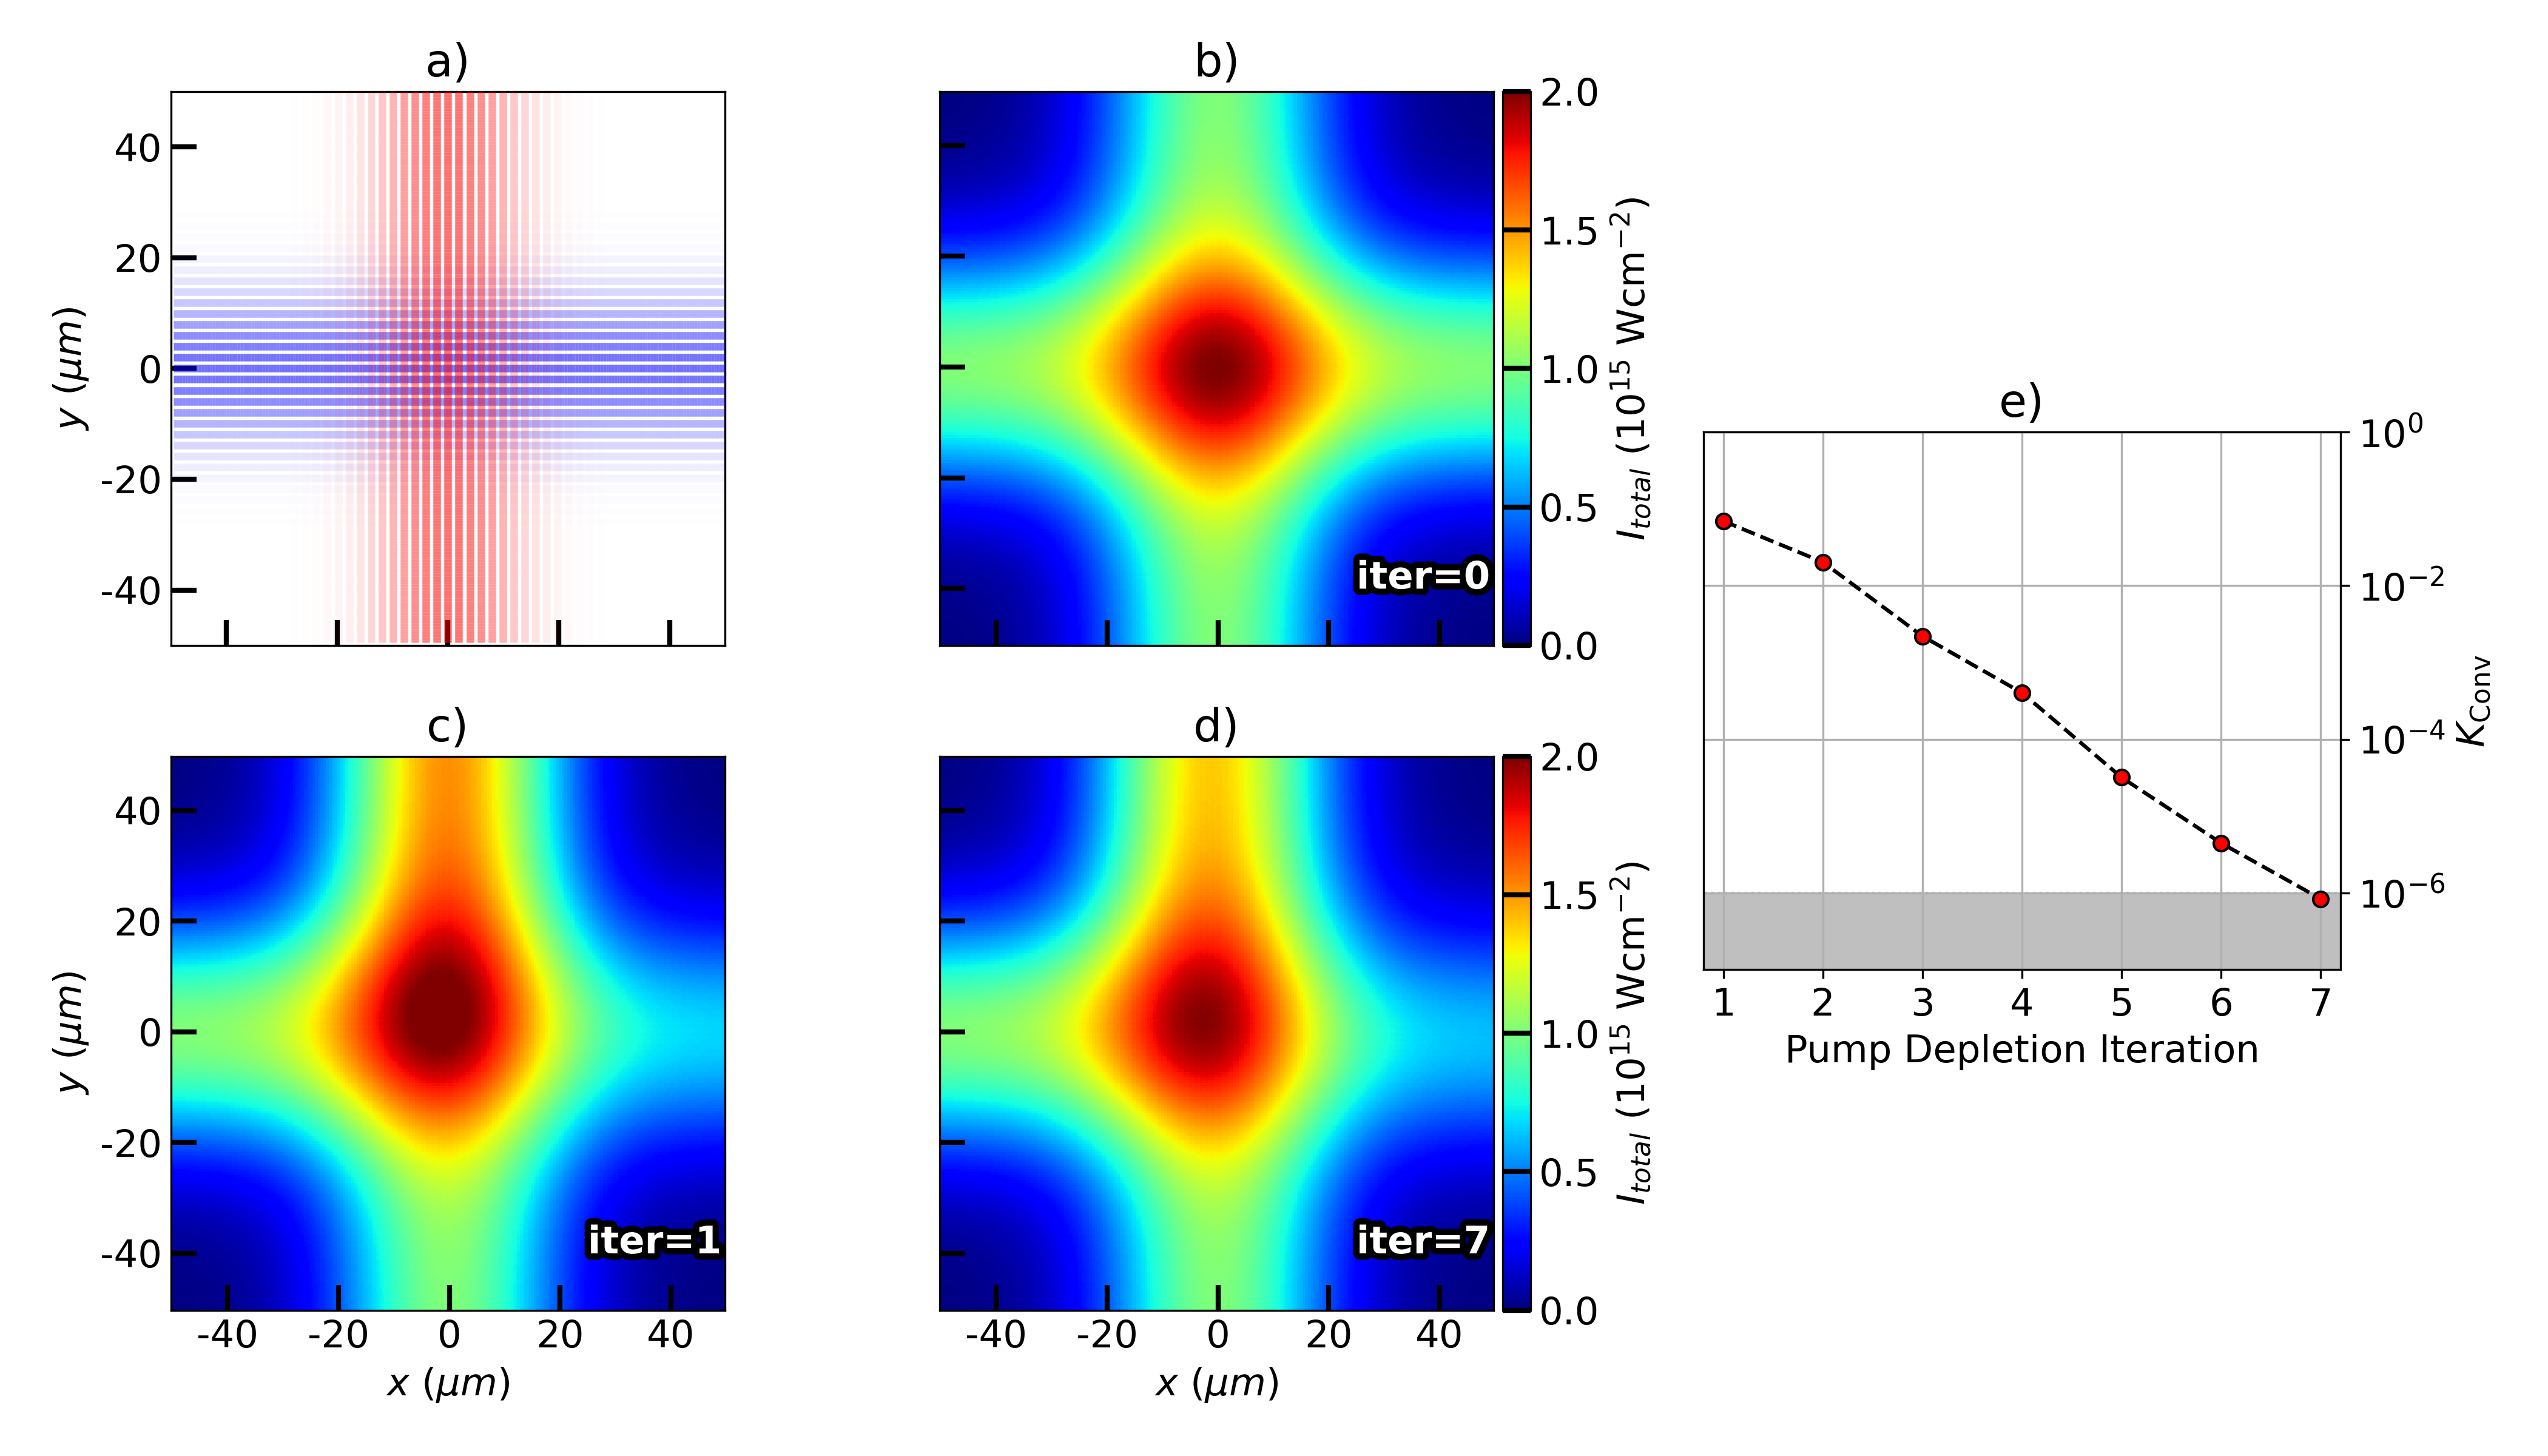
\includegraphics[width=1.0\linewidth]{Numerics/Images/PumpDepletionIterations.png}
    \centering
    \caption{Results of successive pump depletion iterations for an illustrative simulation of two beams crossing and undergoing a \ac{CBET} resonance in a uniform plasma background.
    Each beams' rays from the field reconstruction ray-trace are plotted in a), where more opaque rays indicate a higher power.
    Panel b) plots the reconstructed intensity from this ray-trace, where $i=0$ indicates the field reconstruction ray-trace and therefore no \ac{CBET} occurs.
    Panels c) and d) plot the intensity reconstructed from the $1^{\text{st}}$ and $7^{\text{th}}$ pump depletion iterations respectively, where the effect of transfer of powers between beams due to \ac{CBET} is evident.
    Panel e) plots the convergence parameter from the simulation over successive pump depletion iterations, with convergence defined here as $K_{\text{Conv},0}=10^{-6}$.}%
    \label{fig:PumpDepIters}
\end{figure}

The field reconstruction ray-trace (the initial ray-trace performed in the absence of \ac{CBET}) returns the field from each sheet $|E_j^{i=0}|(\vec{x},\vec{k},\omega,\phi)$, where $j$ is the sheet index and $i=0$ indicates the field reconstruction ray-trace.
This field is discretised on the \textsc{Solas} mesh using nearest neighbour interpolation, so that a ray passing through a cell updates the field in that cell.
Rays can then be re-traced through this mesh and undergo changes in power due to \ac{CBET} interactions with the fields from other sheets.
The solution obtained from a single ray-trace with \ac{CBET} is not the true solution however, because the field that the rays see throughout the \ac{CBET} ray-trace is not dynamically updated by the change in ray power due to \ac{CBET} as they propagate.
This necessitates iteratively solving the ray-trace to account for \ac{CBET} in \textit{pump depletion iterations}, whereby for iteration $i$, the rays from sheet $j$ propagate through the mesh and undergo \ac{CBET} through $|E_{sheet\neq j}^{i-1}|$, while building up a new field, $|\tilde{E}_{j}^{i}|$.
The new \textit{build-up} fields, $|\tilde{E}_{j}^{i}|$, are introduced for the next iteration.
This loop is repeated until convergence of the field has been achieved.
Convergence is tested each iteration ($i>0$) against the total power of rays $\tilde{P}_{j,n}^{i}$, from each sheet $j$ travelling through each cell, explicitly defined by the convergence parameter,
\begin{equation}
    K_{\text{Conv}}^i = \max_{\substack{j\in \text{sheets} \\ n\in \text{cells}}} \left| \left( \tilde{P}_{j,n}^{i}/\tilde{P}_{j,n}^{i-1} \right) -1 \right| < K_{\text{Conv},0},
\end{equation}
where $K_{\text{Conv},0}$ is a user defined parameter, typically set to $10^{-5}$ unless stated otherwise.

This procedure is illustrated in Fig.~\ref{fig:PumpDepIters} for a simple, illustrative problem of two beams crossing in a uniform, stationary plasma background with a frequency difference between the beams tuned to give a \ac{CBET} resonance.
The effect of \ac{Inv-Brem} deposition has been neglected in this simulation.
Fig.~\ref{fig:PumpDepIters}.a shows the ray trajectories for the two crossing beams and Fig.~\ref{fig:PumpDepIters}.b plots the intensity from the field reconstruction iteration, without \ac{CBET}.
The intensities after one and seven pump depletion iterations are plotted in Fig.~\ref{fig:PumpDepIters}.c and Fig.~\ref{fig:PumpDepIters}.d respectively, which show that a single re-trace through the no-\ac{CBET} fields does not return the converged solution.
Fig.~\ref{fig:PumpDepIters}.e plots the convergence parameter after each iteration, illustrating that seven iterations were required to obtain the converged solution, plotted in Fig.~\ref{fig:PumpDepIters}.d.

For many beam simulations with complicated beam trajectories and many overlapping crossings such as direct-drive calculations, the problem is asymptotically unstable.
This means that for iteration $i$, allowing rays to undergo \ac{CBET} in the full $|\tilde{E}_{sheet\neq j}^{i-1}|$ causes unbounded gains on ray powers leading to divergent results for $|\tilde{E}_{j}^{i}|$.
Numerical damping is therefore applied for these calculations to stabilise the solution.
The actual fields that a ray will see for the subsequent iteration, $i+1$, are composed of the weighted sum of the two \textit{build-up} fields,
\begin{equation}
    |E_{j}^{i}| = f_{\text{damp}}|\tilde{E}_{j}^{i}| + (1-f_{\text{damp}})|\tilde{E}_{j}^{i-1}|,
\end{equation}
where $f_{\text{damp}}$ is a user-defined damping value, which is by default set to a (relatively conservative) value of $0.75$, to ensure that the solver does not diverge for complex problems.

%################################################################################
%################################################################################
\subsection{Energy Conservation Iterations}%
\label{sec:energy_conserv_iters}

\begin{figure}[t!]
    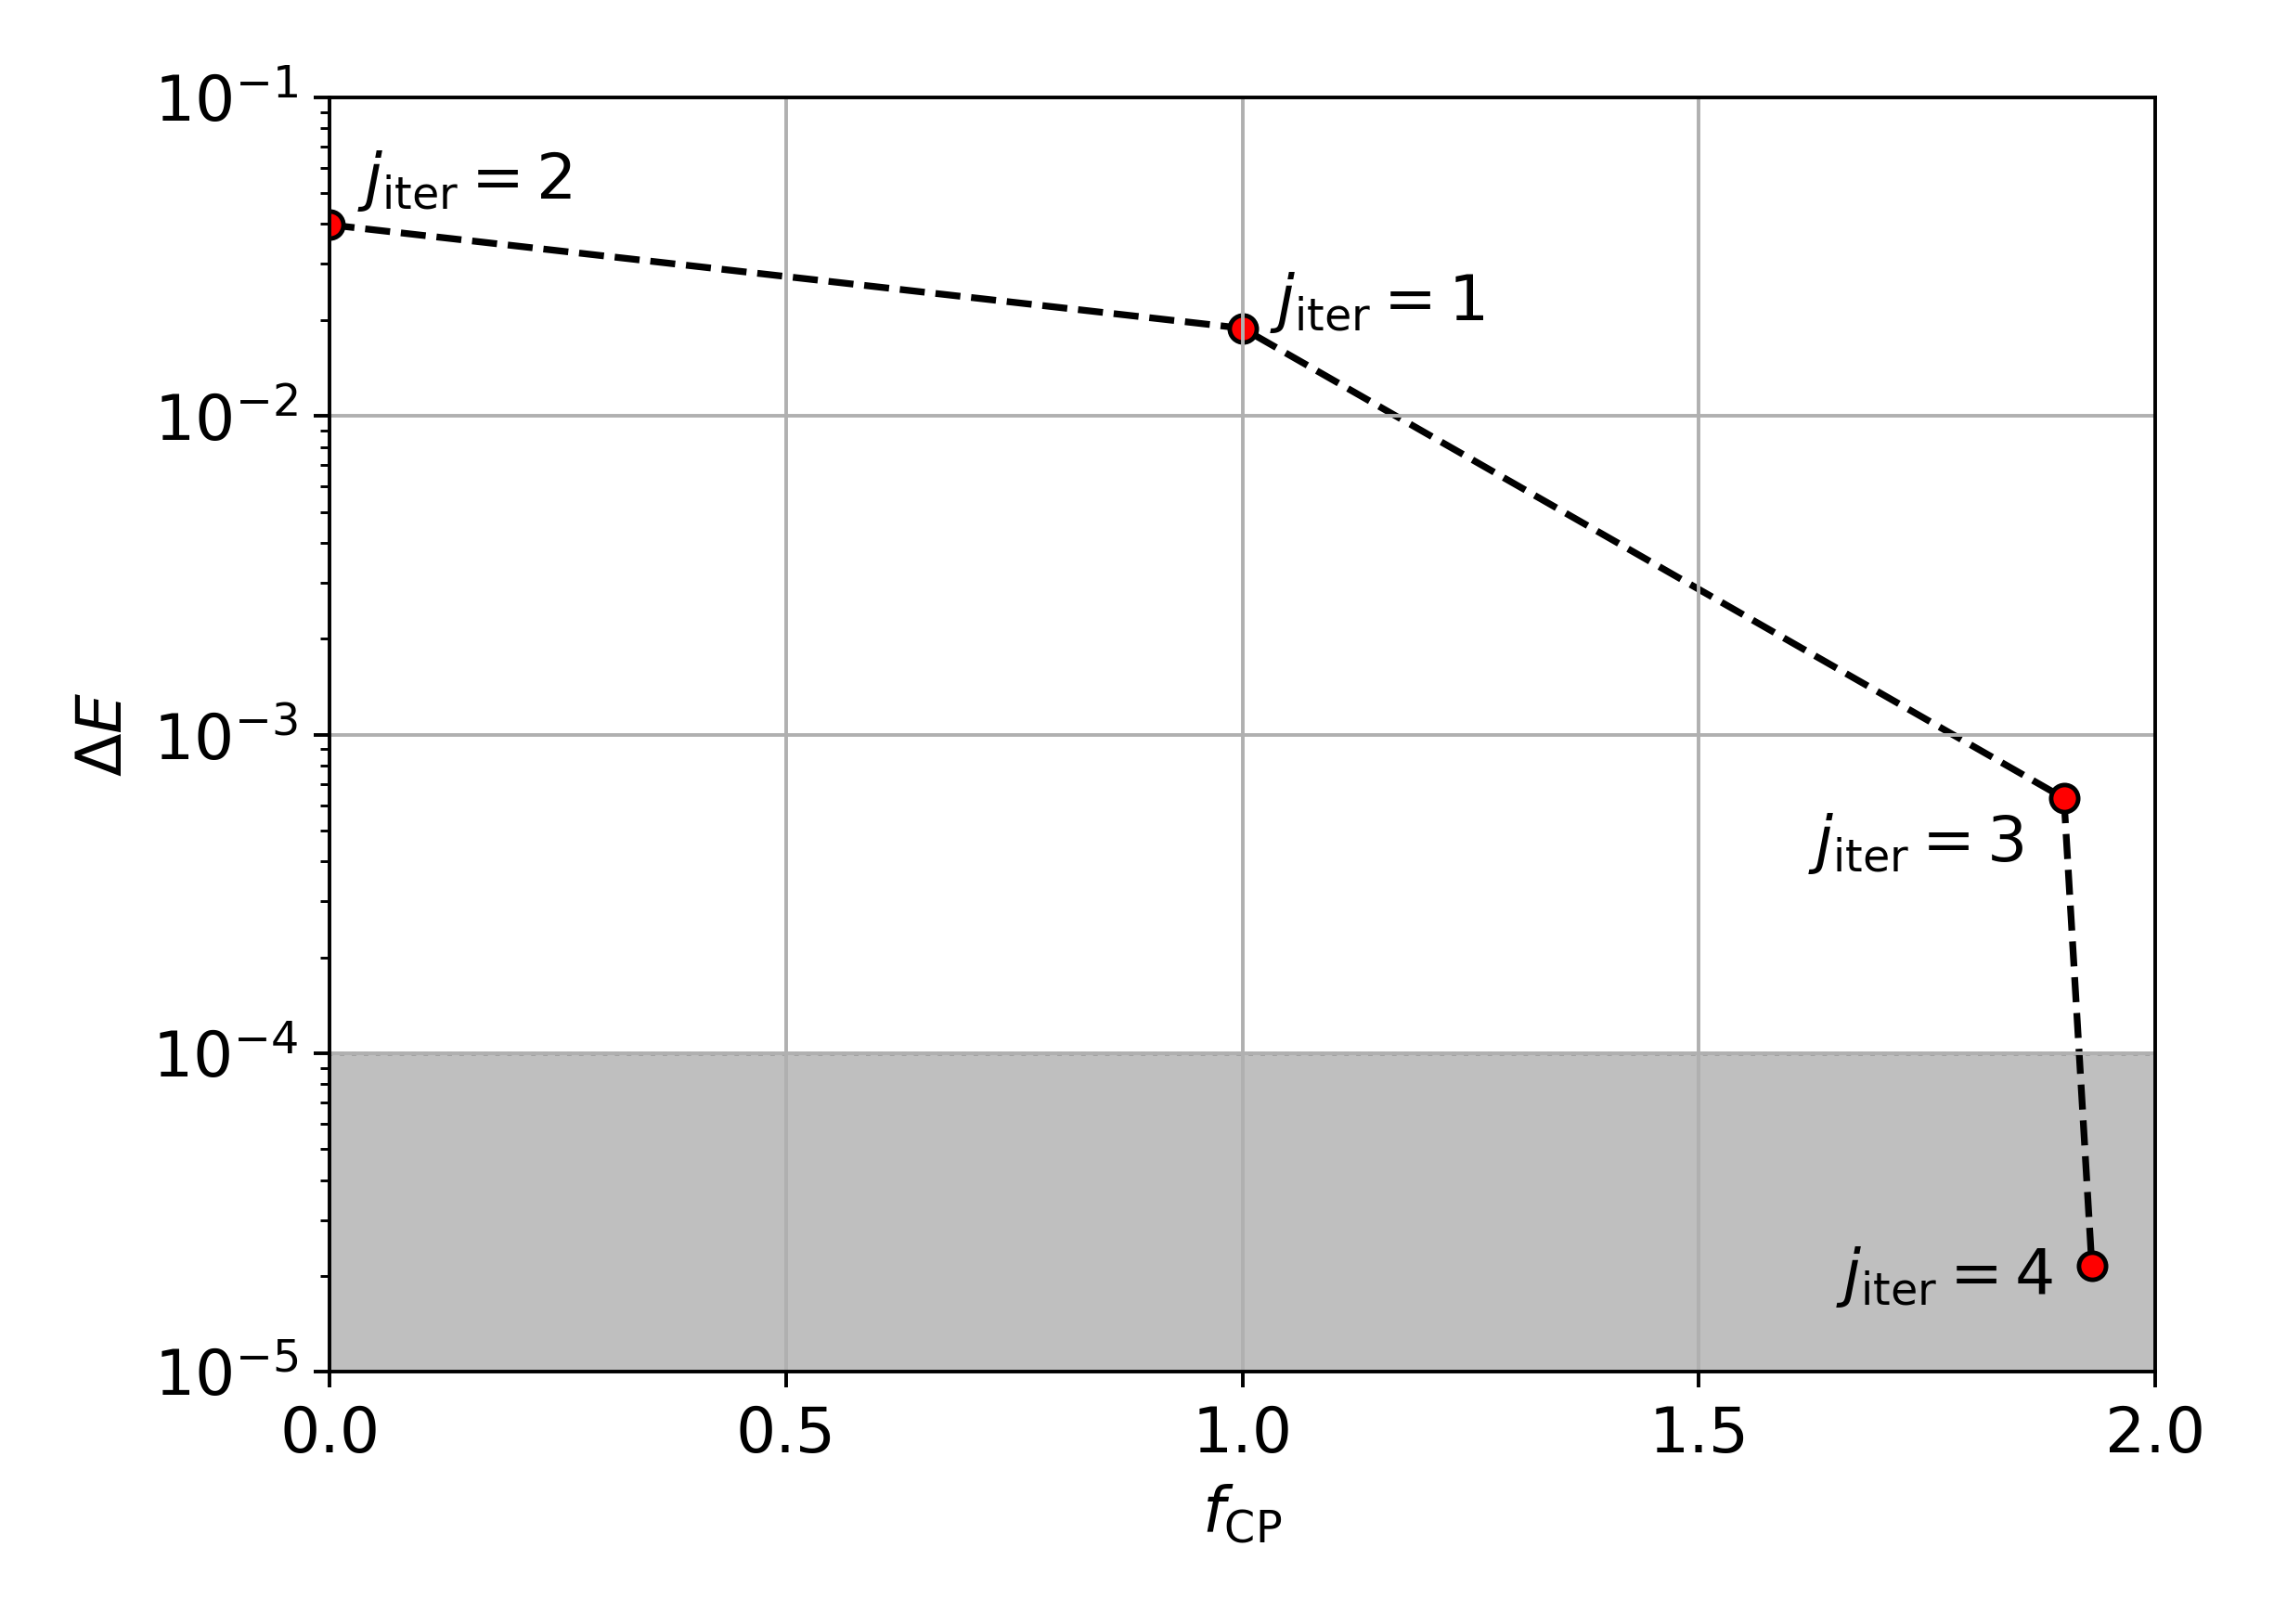
\includegraphics[width=0.6\linewidth]{Numerics/Images/delE_minimisation.png}
    \centering
    \caption{Energy conservation iterations for a two-beam caustic test problem, which is presented in Sec.~\ref{sec:SOLAS_CBET_caustic_test}.
    4 iterations were required to achieve energy conservation, which was defined to be $\delta E<1\times 10^{-4}$.
    The order of the iterations is indicated by the text next to each point.}%
    \label{fig:SOLAS_delE_minimisation}
\end{figure}

The converged field solution from the pump depletion iterations returns the steady-state field and deposition profiles, accounting for \ac{CBET}, given a field reconstruction algorithm, interpolation scheme \textit{etc}.
If there are errors in, for example, the field reconstruction algorithm, then the pump depletion iterations will return a steady-state solution, however this is not guaranteed to be accurate, \textit{i.e.} the same as the result from a higher fidelity solver.
The main cause of errors in field reconstruction is the treatment of laser caustics, as demonstrated for example in Fig.~\ref{fig:SOLAS_2d_field_test}.
This figure demonstrates that the \textsc{Solas} field reconstruction algorithm obtains essentially perfect agreement with \textsc{Lpse} everywhere apart from in the vicinity of the caustic.
It can therefore be assumed that any errors in the \ac{CBET} profiles, returned from the pump depletion iterations, occur due to errors in the field reconstruction and \ac{CBET} scattering in the caustic region.
The energy conservation error, $\Delta E$, is a good proxy for the accuracy of the fields obtained from \ac{CBET}, as in the absence of laser caustics, energy is conserved in ray-based algorithms~\cite{follett_validation_2022}.
This is defined as,
\begin{equation}
    \Delta E = \frac{ P_{\text{dep}} + P_{\text{out}} - P_{\text{inc}} }{ P_{\text{inc}} },
\end{equation}
where $P_{\text{dep}}$, $P_{\text{out}}$ and $P_{\text{inc}}$ are the power deposited by \ac{Inv-Brem}, the ray-power leaving the domain and the incident power respectively.
If this value is not small, it suggests that caustics are not accurately treated in the \ac{CBET} scattering.

As in the \textsc{BeamCrosser} code, the assumption in \textsc{Solas} is made that minimising $\Delta E$ by altering the \ac{CBET} gains in the caustic region will bring the result into better agreement with the true solution~\cite{follett_validation_2022}.
$M_{\text{CP}}$ is modified to include a new \textit{caustic pump multiplier}, $f_{\text{CP}}$, which is applied to probe ray \ac{CBET} gains, when they are in the caustic region of the pump sheet,
\begin{equation}
    \label{eq:modified_MCP}
    \tilde{M}_{\text{CP}}= 
\begin{cases}
    1 + f_{\text{CP}} \left( \frac{2}{\pi} \right),& \text{if in caustic region}\\
    1,              & \text{otherwise}
\end{cases}
\end{equation}
where the same, geometric identification for the pump sheet caustic region is used as in Sec.~\ref{sec:SOLAS_coherent_caustic}.
$f_{\text{CP}}=1$ initially and is varied between $f_{\text{CP}}\in [-\pi/2,2]$ over several \textit{energy conservation} iterations\footnote{Each energy conservation iteration contains a new set of pump depletion iterations, as is shown in Fig.~\ref{fig:SOLAS_CBET_flowchart}.} to minimise $\Delta E$.
The lower bound on $f_{\text{CP}}$ is to prevent `negative scattering' in the caustic region, where the sign of the gain flips.
The upper bound was selected by experimentation to prevent excessively large gains which result in the exponential power gain of rays blowing up to infinity.

An implementation of the Secant method is used to estimate the next value of $f_{\text{CP}}$.
The first and second energy conservation iterations in a simulation use $f_{\text{CP}}=1$ and $0$, to obtain a gradient with which to estimate values of the multiplier.
The Secant method was chosen for its simplicity and the fact that bracketing values of the root are not required.
An example of the minimisation results are shown in Fig.~\ref{fig:SOLAS_delE_minimisation}.
These results are from a two-beam caustic test problem, presented in Sec.~\ref{sec:SOLAS_CBET_caustic_test}, but the specifics of the problem are not important for the discussion here, simply that \ac{CBET} in the presence of a caustic occurs.
Therefore, a caustic region exists inside which $f_{\text{CP}}$ will lead to modified gains which reduce energy conservation errors.
The curve of $\Delta E(f_{\text{CP}})$ is simple and monotonic, which is observed for all simulations conducted with \textsc{Solas}, regardless of the complexity of the laser and target configuration.
This means a more complex algorithm than the Secant method is not required for minimisation.
When the \ac{CBET} model runs in-line with the hydrodynamics, the value of $f_{\text{CP}}$ from the last timestep that \ac{CBET} was calculated is used, which means that energy conservation iterations are often not necessary.
This is shown explicitly in Fig.~\ref{fig:SOLAS_89224}.c, which shows the results of a 1-D \textsc{Chimera}-\textsc{Solas} simulation of \textsc{Omega} shot 89224.
The bottom panel in the figure shows that energy conservation is frequently achieved by simply re-using the value of $f_{\text{CP}}$ from the previous timestep.

To summarise, the total \ac{CBET} gain that a probe ray ($i$) experiences in a pump sheet ($j$) is,
\begin{equation}
    \tilde{\gamma}_{ij} = \gamma_{ij} M_{\text{PS}} \tilde{M}_{\text{CP}},
\end{equation}
where $\gamma_{ij}$ is the value defined in Sec.~\ref{sec:SOLAS_ray_power_change} (depending on if using the kinetic or fluid gain model), the modified coherent caustic multiplier $\tilde{M}_{\text{CP}}$ is defined in Eq.~\ref{eq:modified_MCP} and the polarisation smoothing multiplier, $M_{\text{PS}}$, defined in Eq.~\ref{eq:polarisation_smoothing}, is applied if the beams are assumed to be randomly rather than parallel-polarised.

%################################################################################
%################################################################################
\subsection{CBET Validation}

This section presents results from several \ac{CBET} test problems where the results from \textsc{Solas} are compared to the wave based solver \textsc{Lpse}.
Because \textsc{Lpse} is a wave-solver coupled to a linearised fluid response, the fluid \ac{CBET} gain was used for all simulations in this section.
Beams in the simulations all had a vacuum wavelength, $\lambda_0=0.351\ \text{nm}$ and a super-Gaussian spot profile, which was defined in Eq.~\ref{eq:supgaus}.
For consistency with \textsc{Lpse}, the Doppler shift of laser frequency was not calculated in these simulations so its effect on \ac{CBET} is neglected, \textit{i.e.} the right-hand side of Eq.~\ref{eq:SOLAS_doppler_used} was forced to be zero.
The plasma backgrounds for all initialisations were fully-ionised CH with $Z=3.1$ and $T_i=T_e/2$.
All tests are presented in Ref.~\cite{follett_validation_2022} and the \textsc{Lpse} data is available from the repository in Ref.~\cite{follett_lpse_2022}.

%##################################################
\subsubsection{2-D CBET Without Caustics}

\begin{figure}[t!]
    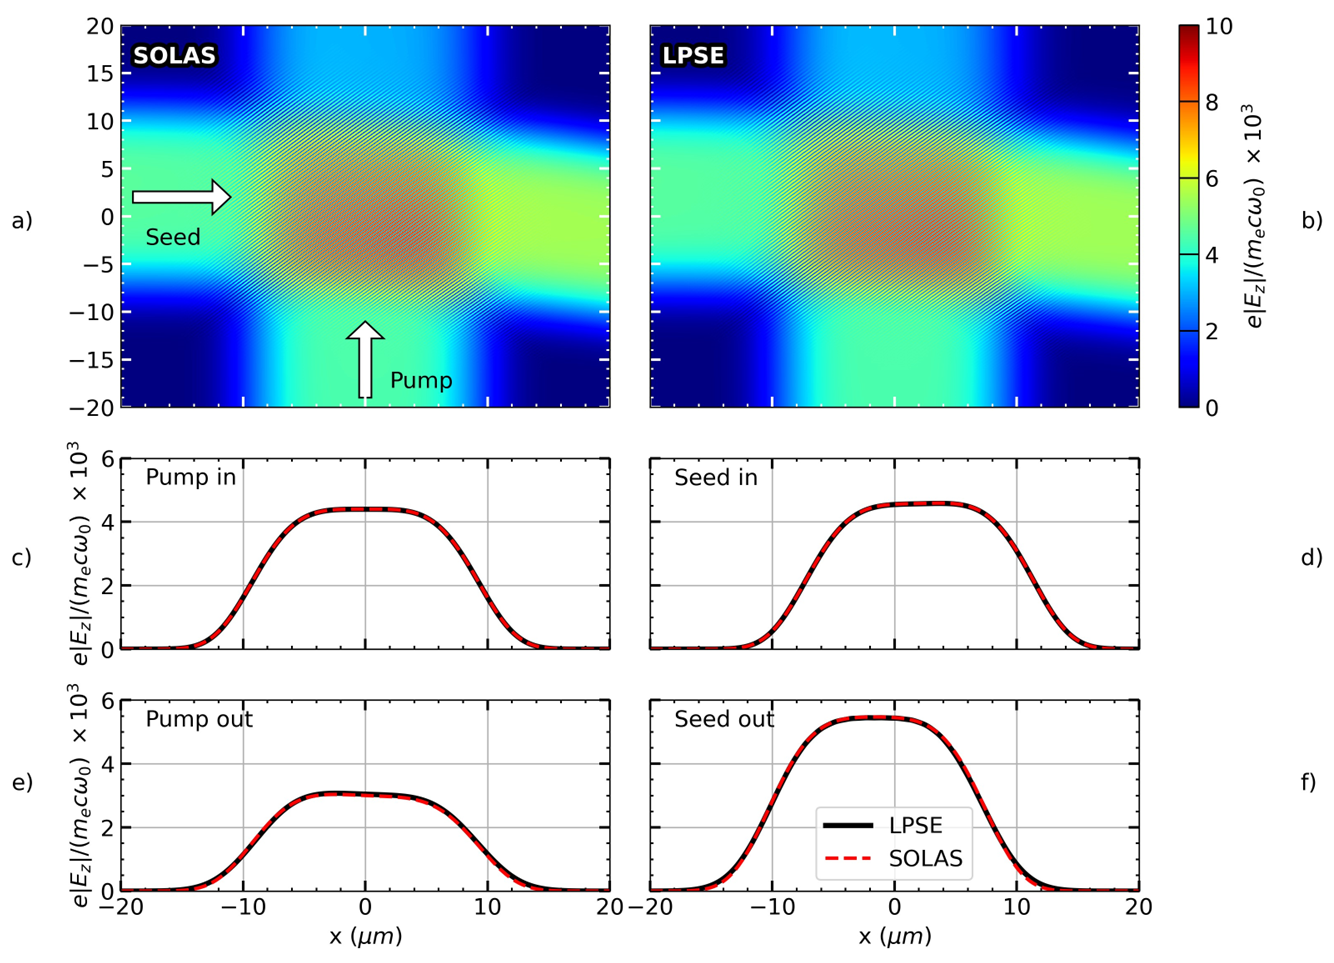
\includegraphics[width=1.0\linewidth]{Numerics/Images/CBET_test_nocaustics.png}
    \centering
    \caption{Results of the 2-D \ac{CBET} test in the absence of laser caustics.
    Panels a) and b) show the electric field from the \textsc{Solas} and \textsc{Lpse} simulations respectively, after the pump depletion iterations have occurred.
    Panels c) and d) plot lineouts from the inbound fields of the pump and seed beams respectively for both \textsc{Solas} and \textsc{Lpse}.
    e) and f) plot the same for the outbound fields.}%
    \label{fig:SOLAS_CBET_test_nocaustics}
\end{figure}

\begin{table}[ht]
    \centering
    \caption{The ratio of the power of the seed beam as it exits the domain to its initial power.}
    \begin{tabular}{cccc} \hhline{====}
    & $P_{\text{seed,out}}^{\textsc{Lpse}}/P_{\text{seed,in}}^{\textsc{Lpse}}$ & $P_{\text{seed,out}}^{\textsc{BeamCrosser}}/P_{\text{seed,in}}^{\textsc{BeamCrosser}}$ & $P_{\text{seed,out}}^{\textsc{Solas}}/P_{\text{seed,in}}^{\textsc{Solas}}$ \\ 
    \midrule
    CBET + Absorption & 1.315 & 1.325 & 1.320 \\
    CBET only & 1.551 & 1.561 & 1.558 \\
    Absorption only & 0.856 & 0.856 & 0.852 \\ \hhline{====}
    \end{tabular}%
    \label{tab:nocaustic_CBET_table}
\end{table}

The first test problem is for the case of two beams crossing in a non-uniform, non-stationary plasma in the absence of laser caustics.
The grid used for the problem was $x,y \in [-21,22]\ \mu\text{m}$ and 2160 cells were used in each direction.
This led to a resolution of $\Delta x\sim \lambda_0/20$ such that the beat field between the two beams could be resolved.
The electron temperature was uniform, $T_e=1\ \text{keV}$.
The density and fluid velocity profiles were,
\begin{align}
    n_e(y) &= n_{\text{cr}} (0.006y_{\mu\text{m}} + 0.25), \\
    \vec{u}(y) &= -\hat{\vec{y}}(1.4-0.008y_{\mu\text{m}})c_s,
\end{align}
where $y_{\mu\text{m}}$ is the coordinate in microns.
The beams both had widths $\sigma=8.41\ \mu\text{m}$ and peak intensities $I_0 = 2\times 10^{18}\ \text{W}/\text{m}^{2}$.
The beams were defined as \textit{pump} and \textit{seed} and launched from $\vec{x} = [-21,2]\ \mu\text{m}$ and $\vec{x} = [0,-21]\ \mu\text{m}$ along the $+\hat{\vec{x}}$ and $+\hat{\vec{y}}$ directions respectively.
The beam and plasma configuration were chosen to create a strong \ac{CBET} resonance where the beams cross one another.

Fig.~\ref{fig:SOLAS_CBET_test_nocaustics}.a and Fig.~\ref{fig:SOLAS_CBET_test_nocaustics}.b show the electric field obtained from the \textsc{Solas} and \textsc{Lpse} simulations respectively.
It can be seen that the density gradient in $\hat{\vec{y}}$ causes the seed beam to refract somewhat and that \ac{CBET} results in a significant energy transfer from the pump to the seed beam.
The lineouts in Fig.~\ref{fig:SOLAS_CBET_test_nocaustics}.c, Fig.~\ref{fig:SOLAS_CBET_test_nocaustics}.d, Fig.~\ref{fig:SOLAS_CBET_test_nocaustics}.e and Fig.~\ref{fig:SOLAS_CBET_test_nocaustics}.f all show excellent agreement between \textsc{Solas} and \textsc{Lpse}.
This is further demonstrated in Tab.~\ref{tab:nocaustic_CBET_table}, which lists the ratio of the outgoing seed beam power to the incident power for \textsc{Lpse}, \textsc{Solas} and the \textsc{BeamCrosser} post-processor, the results from which are also presented in Ref.~\cite{follett_validation_2022}.
The energy conservation error after the pump depletion iterations was small, $\Delta E \sim 10^{-6}$, as expected because the \ac{CBET} interaction does not involve any caustics.

%##################################################
\subsubsection{2-D CBET With Caustics}%
\label{sec:SOLAS_CBET_caustic_test}

\begin{figure}[t!]
    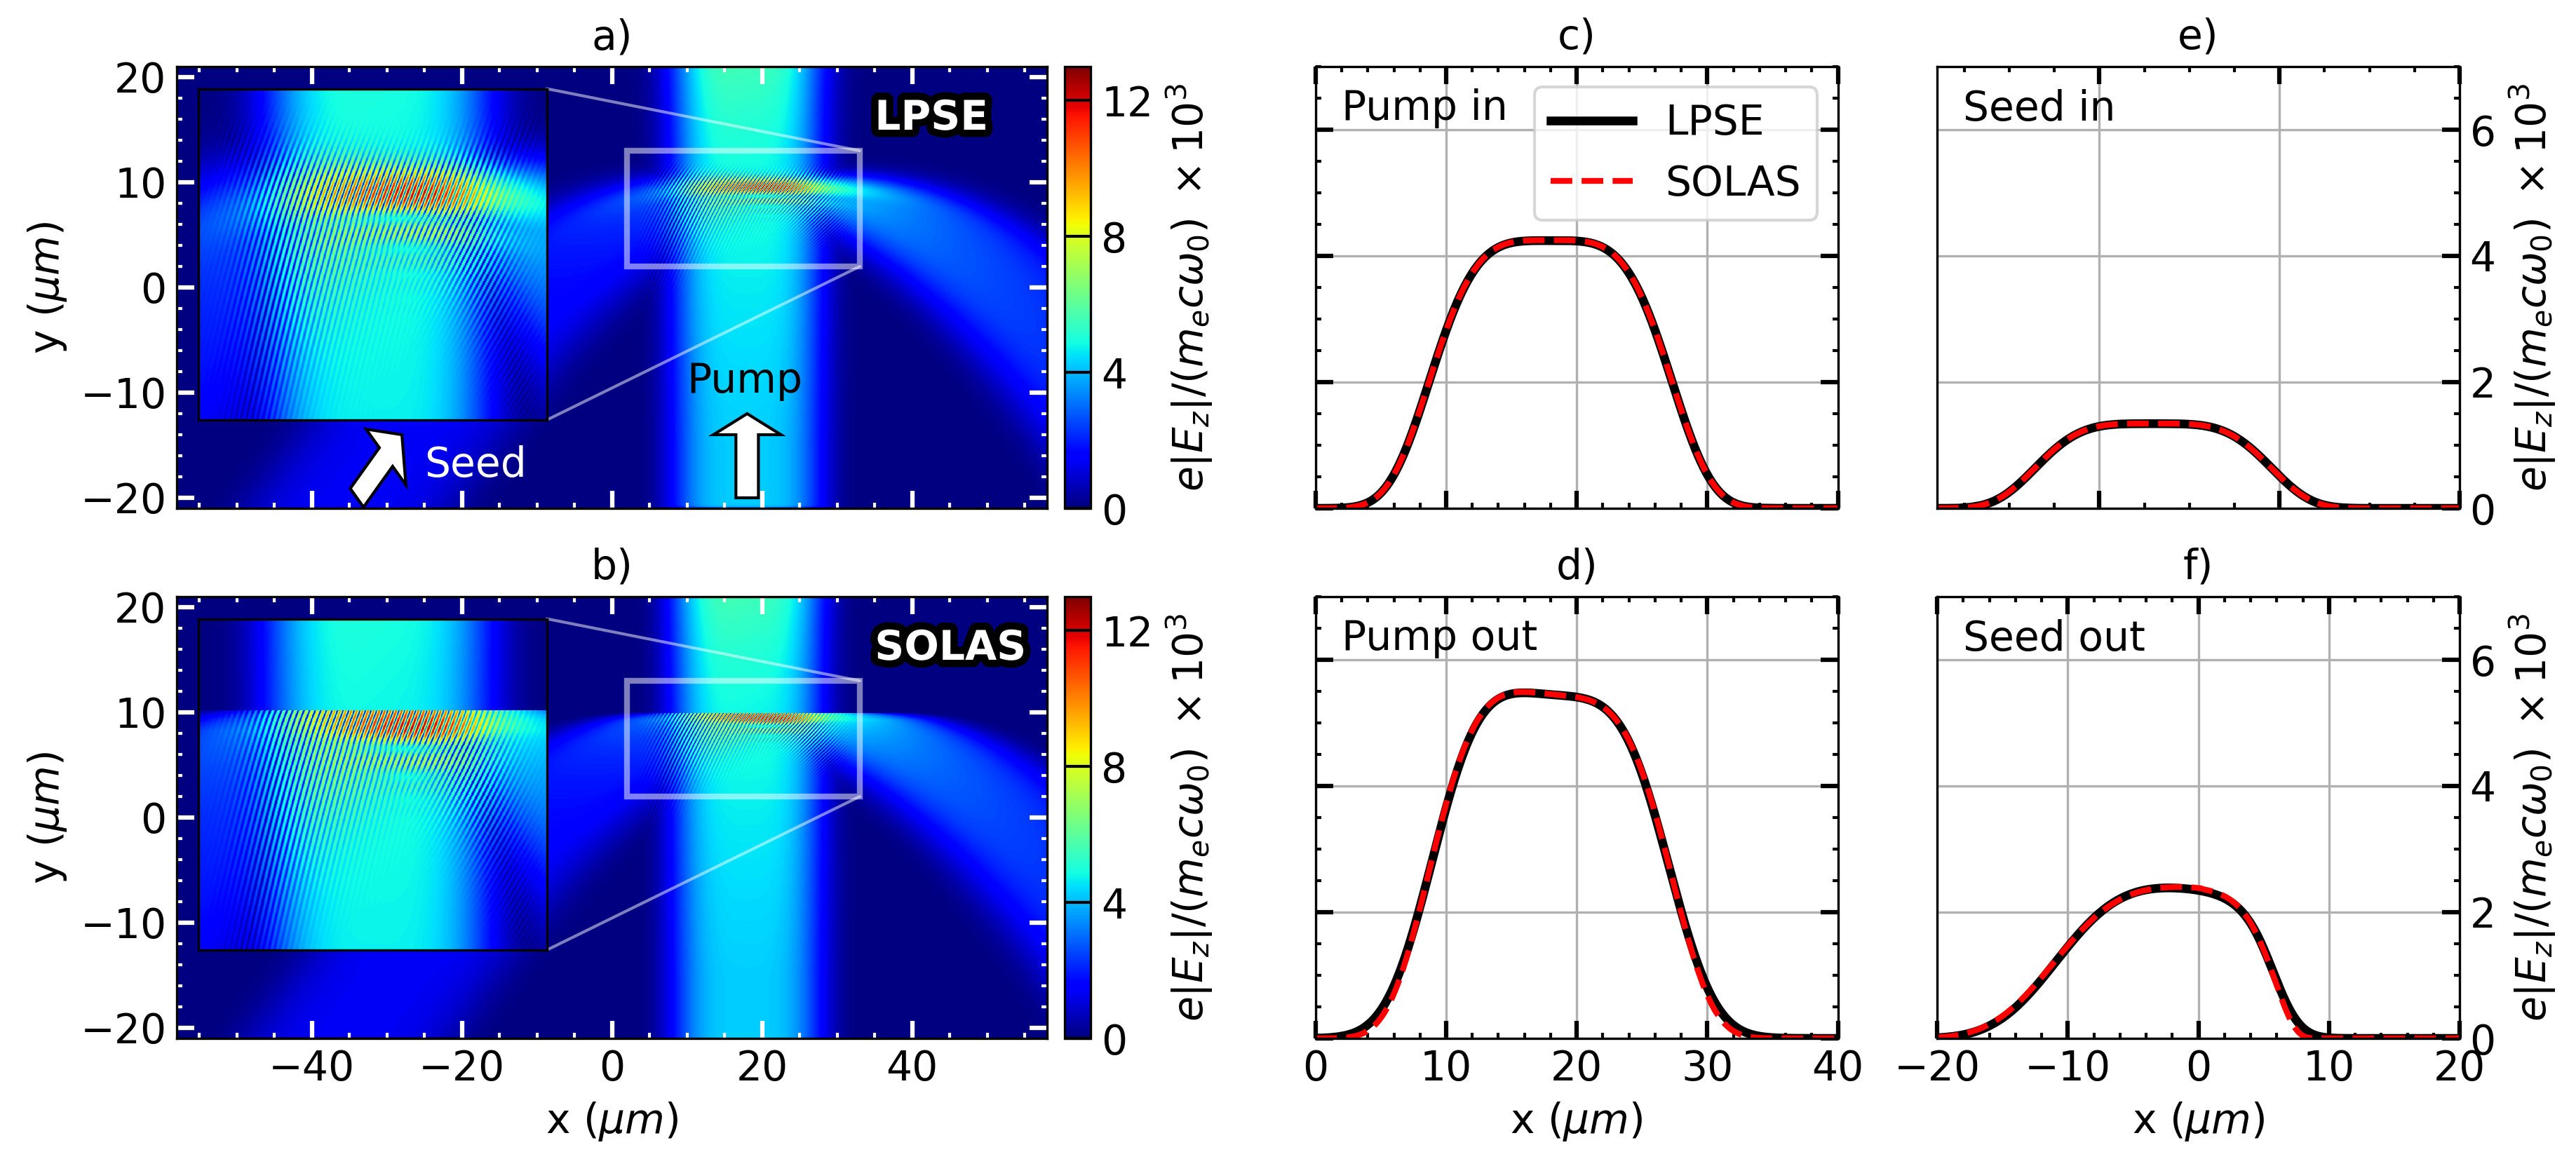
\includegraphics[width=1.0\linewidth]{Numerics/Images/caustic_CBET_test.png}
    \centering
    \caption{Results of the 2-D \ac{CBET} test in the presence of a laser caustic.
    Panels a) and b) show the electric field from the \textsc{Lpse} and \textsc{Solas} simulations respectively.
    Also plotted is an inset zoom on the caustic region of the seed beam, which demonstrates that \textsc{Solas} does not capture the evanescent field.
    Panels c) and e) plot lineouts from the inbound fields of the pump and seed beams respectively for both \textsc{Solas} and \textsc{Lpse}.
    d) and f) plot the same for the outbound fields.}%
    \label{fig:SOLAS_CBET_test_caustics}
\end{figure}

Another two-beam problem was implemented to test \ac{CBET} in the presence of a caustic.
For this simulation, the grid was $x,y \in [-21,21]\ \mu\text{m}$ and $x,y \in [-60,60]\ \mu\text{m}$ with a minimum resolution of $\Delta x = \Delta y \sim \lambda_0/20$.
A uniform electron temperature was used, $T_e=2\ \text{keV}$.
The pump beam travelled straight up a linear density gradient and therefore did not refract, whereas the seed beam reflected in the gradient and travels out.
The beam geometry was chosen so that the pump beam crossed through the middle of the seed beam caustic and the density and flow profiles were tuned to create a resonance at this crossing location,
\begin{align}
    n_e(y) &= 
    \begin{cases}
        0.02y_{\mu\text{m}} + 0.3, & x\geq -15\ \mu\text{m},\\
        0,              & x<-15\ \mu\text{m},
    \end{cases} \\
    \vec{u} &= -1.14 c_s \hat{\vec{y}}.
\end{align}
Both beams again had widths $\sigma=8.41\ \mu\text{m}$.
The pump and seed beams were launched from $\vec{x}=[18,-21]\ \mu\text{m}$ and $\vec{x}=[-35,-21]\ \mu\text{m}$ and pointed along $\hat{\vec{k}}=[0,1]$ and $\hat{\vec{k}}=[0.707,0.707]$ respectively.
The peak intensities were $I_0=2\times10^{18}\ \text{W}/\text{m}^2$ and $I_0=2\times10^{17}\ \text{W}/\text{m}^2$ for the pump and seed respectively.

Fig.~\ref{fig:SOLAS_CBET_test_caustics}.a and Fig.~\ref{fig:SOLAS_CBET_test_caustics}.b plot the \textsc{Lpse} and \textsc{Solas}\footnote{The field from \textsc{Solas} simulation with the minimum resolution, $\Delta x \sim \lambda_0/20$ is plotted in Fig.~\ref{fig:SOLAS_CBET_test_caustics}.b.} total fields respectively.
The inset zooms demonstrate that the evanescent fields are not captured in the \ac{GO} framework.
Fig.~\ref{fig:SOLAS_CBET_test_caustics}.c, Fig.~\ref{fig:SOLAS_CBET_test_caustics}.d, Fig.~\ref{fig:SOLAS_CBET_test_caustics}.e and Fig.~\ref{fig:SOLAS_CBET_test_caustics}.f plot the lineouts of the \textsc{Lpse} and \textsc{Solas} field solutions at their exit from the grid, which all demonstrate excellent agreement.
The \textsc{Lpse} seed beam amplification was $P_{\text{seed,out}}/P_{\text{seed,in}}=1.94$~\cite{follett_validation_2022}.
This test was run both with and without the \ac{CGT} model described in Sec.~\ref{sec:SOLAS_caustic_gain_truncation} and at a variety of resolutions, to demonstrate how energy conservation at caustics are partially a resolution problem and how \ac{CGT} mitigates for this somewhat.

\begin{figure}[t!]
    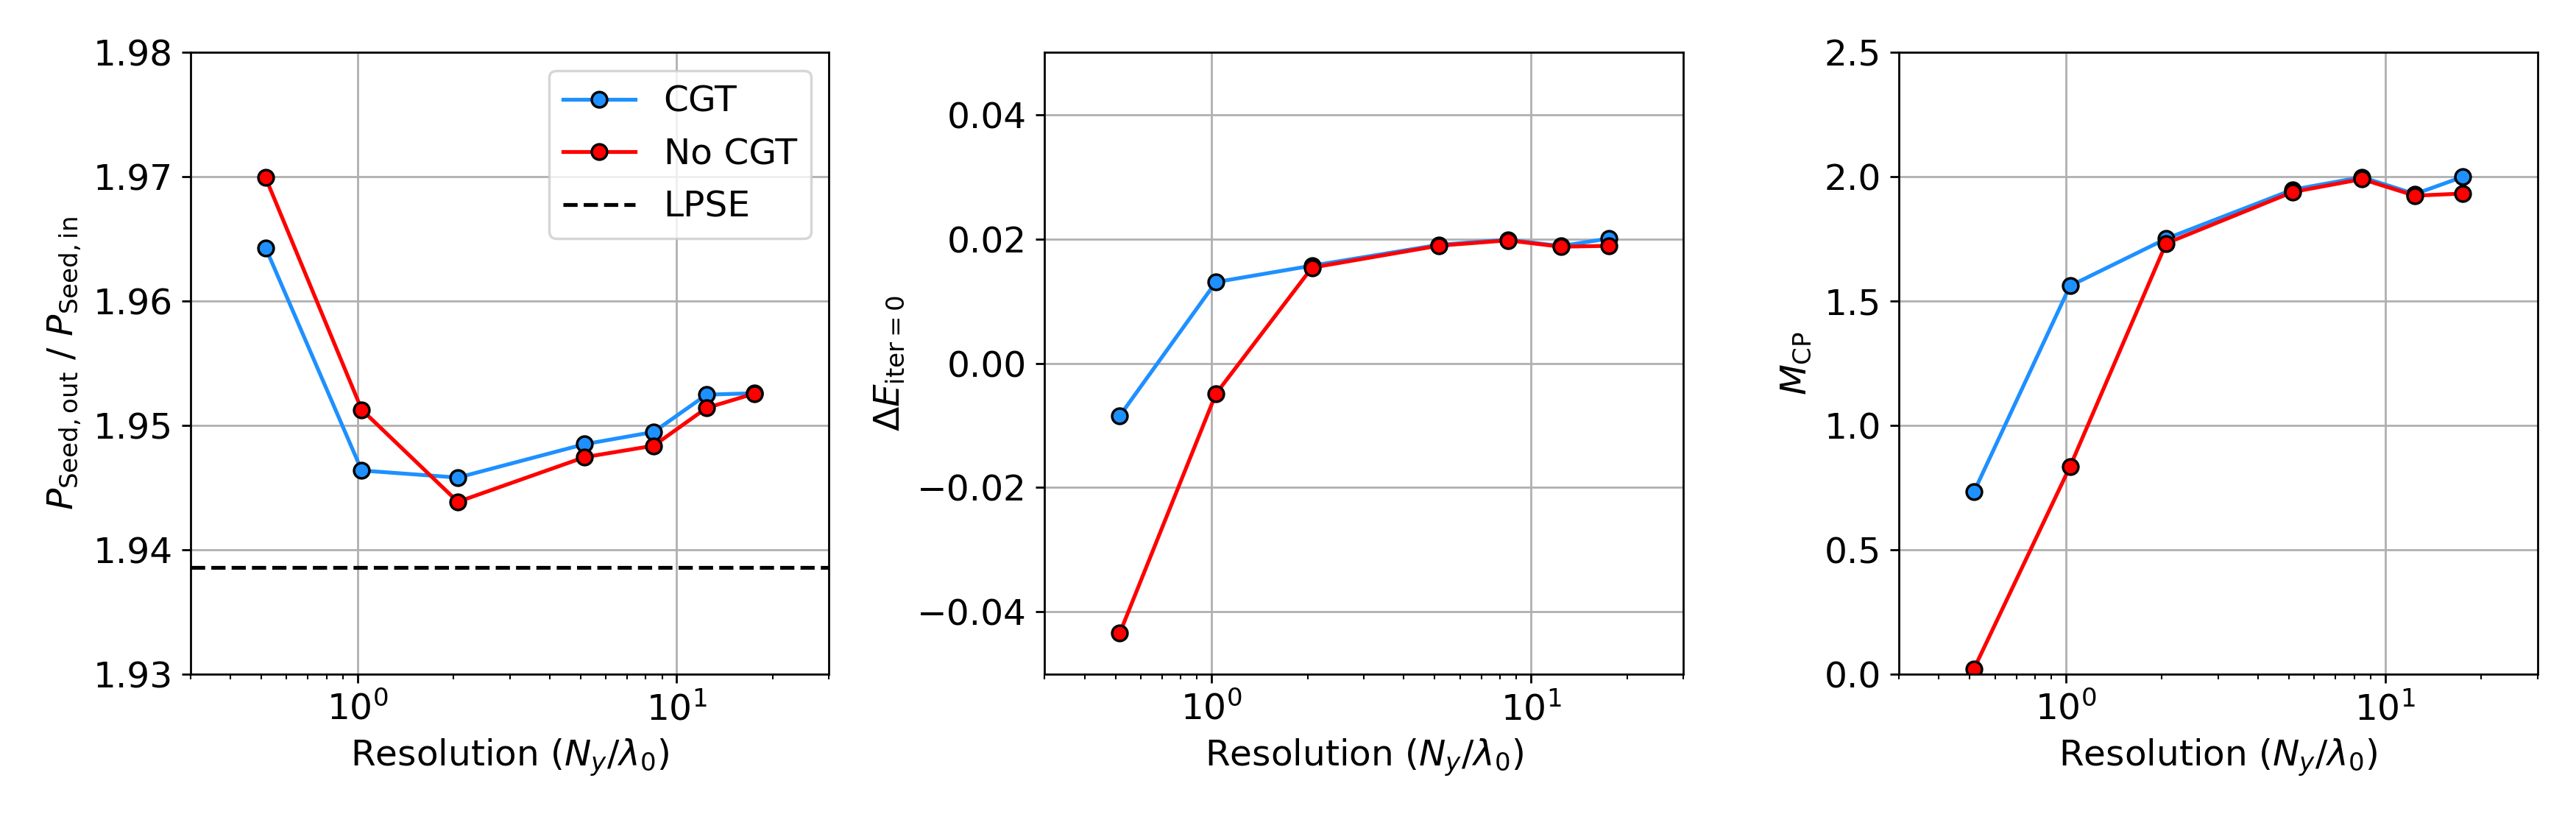
\includegraphics[width=1.0\linewidth]{Numerics/Images/caustic_cbet_test_resscan.png}
    \centering
    \caption{Results from a resolution scan of the two-beam caustic \ac{CBET} test both with \ac{CGT} and without.
    Plotted in a), b) and c) are the power amplification of the seed beam, initial energy conservation error before energy conservation iterations and caustic pump multiplier used to obtain energy conservation respectively.}%
    \label{fig:SOLAS_CBET_test_caustics_resscan}
\end{figure}

Fig.~\ref{fig:SOLAS_CBET_test_caustics_resscan} plots the results of the resolution scans both with and without \ac{CGT}.
The seed beam amplification after energy conservation iterations is plotted in Fig.~\ref{fig:SOLAS_CBET_test_caustics_resscan}.a, which demonstrates that even at lower resolutions, \textsc{Solas} is manages to reproduce the \textsc{Lpse} result to an accuracy of $\mathcal{O}(1\%)$.
The energy conservation error from the first energy conservation iteration (\textit{i.e.} after the first set of pump depletion iterations, but before energy conservation was achieved), is plotted in Fig.~\ref{fig:SOLAS_CBET_test_caustics_resscan}.b.
This plot shows convergence in the physics at higher resolutions, although the converged solution (without enforced energy conservation) indicates small errors in the handling of the caustics, which energy conservation is able to correct in an \textit{ad-hoc} manner.
Fig.~\ref{fig:SOLAS_CBET_test_caustics_resscan}.c plots the caustic pump multiplier that was required to achieve energy conservation.
Both Fig.~\ref{fig:SOLAS_CBET_test_caustics_resscan}.b and Fig.~\ref{fig:SOLAS_CBET_test_caustics_resscan}.c show that \ac{CGT} improves the convergence of the \textsc{Solas} solution when the caustic region width $\sim\lambda_0$ is not properly resolved by the mesh.

%##################################################
\subsubsection{16 Beam CBET in 2-D}%
\label{sec:SOLAS_16beam_CBET}

\begin{figure}[t!]
    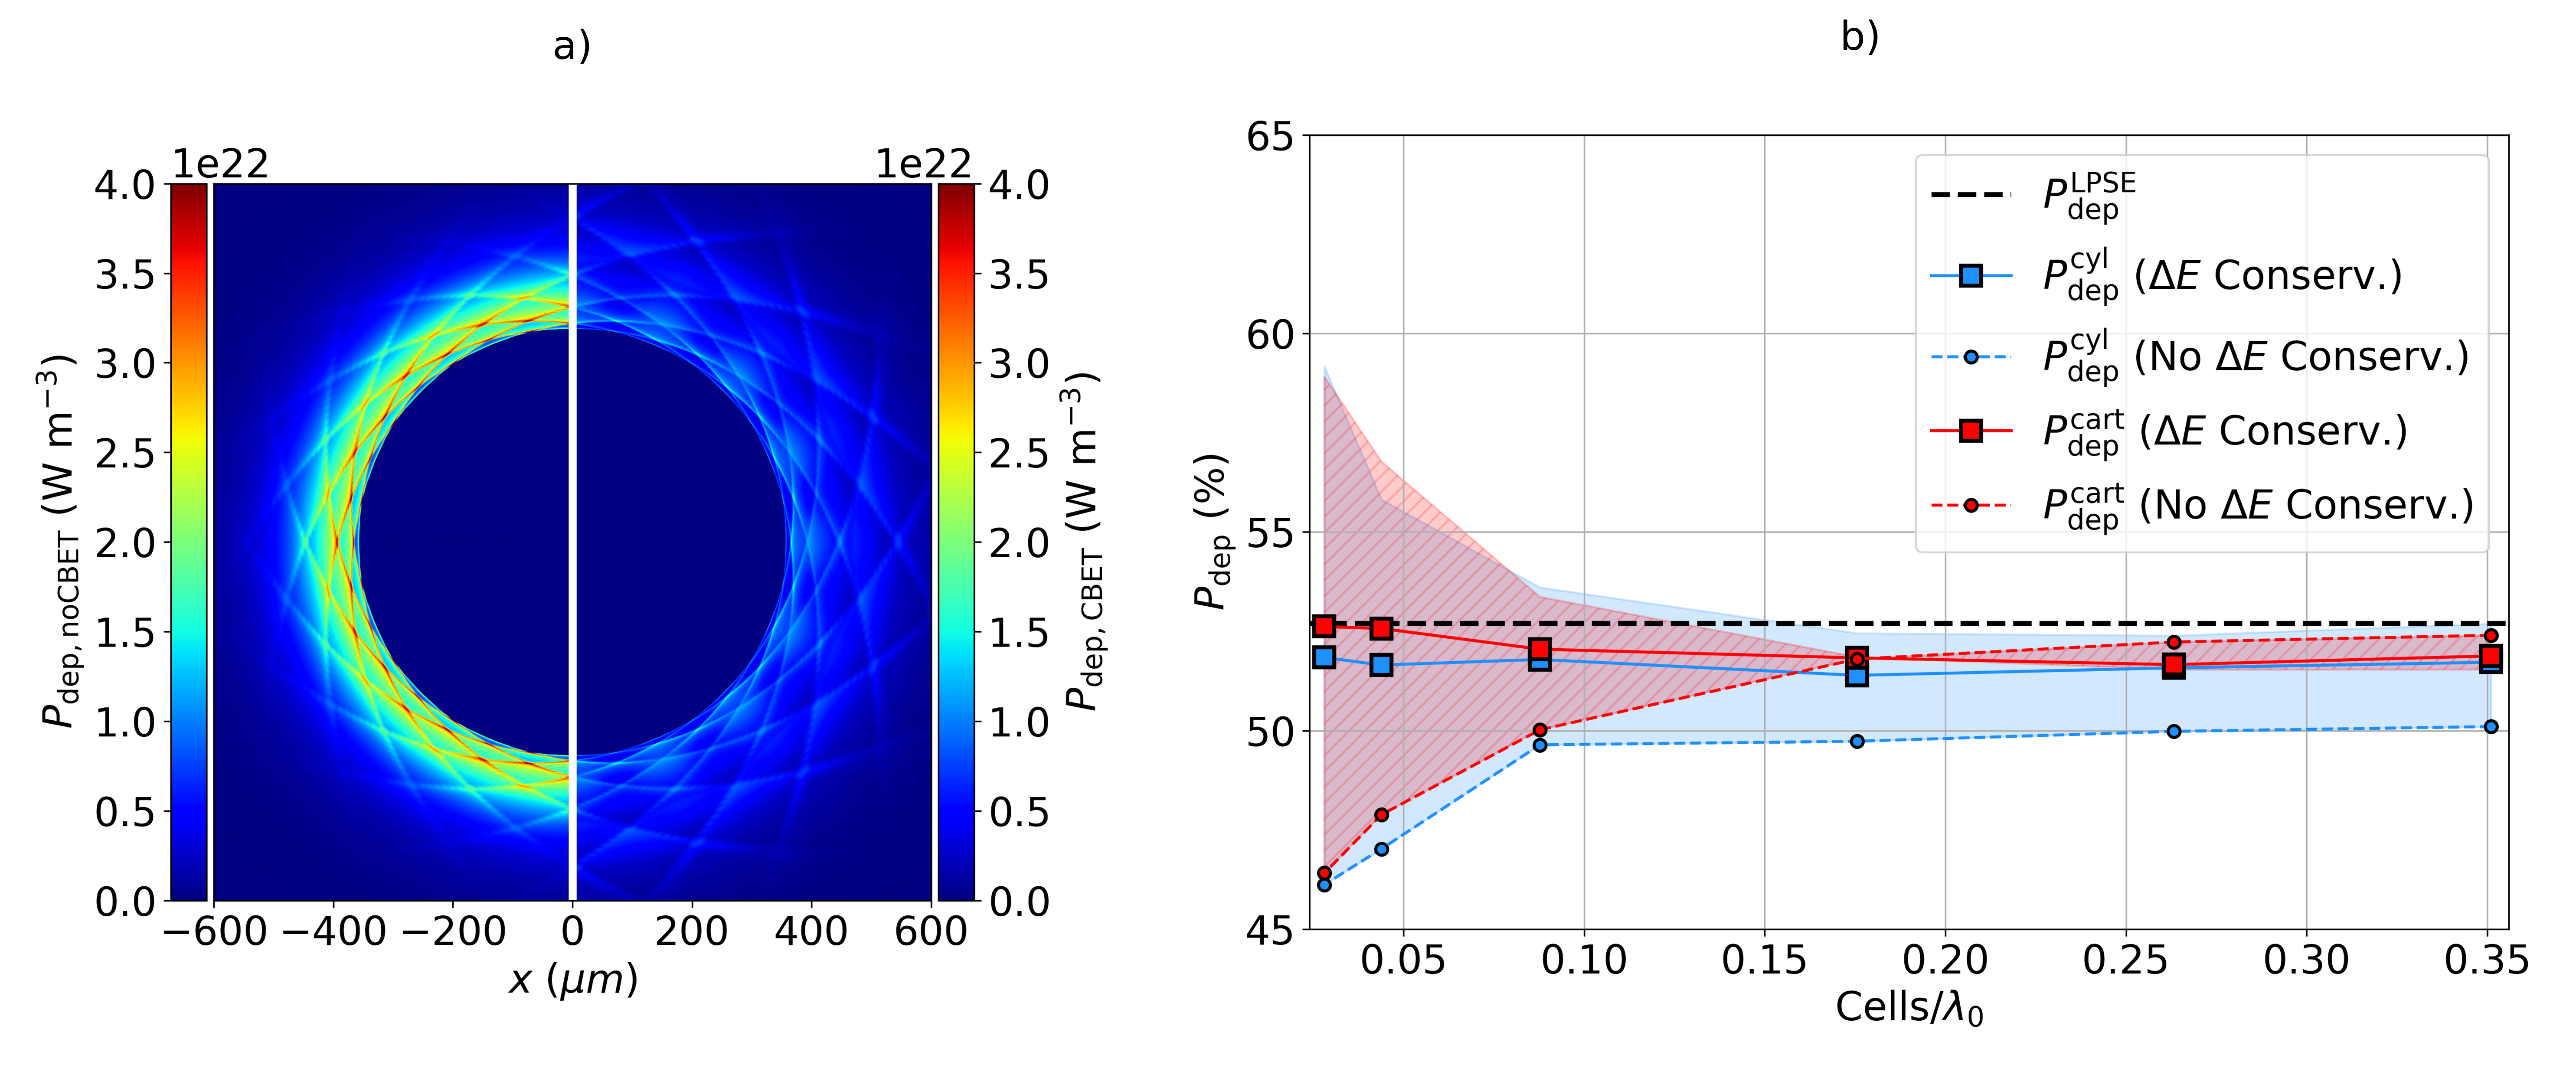
\includegraphics[width=1.0\linewidth]{Numerics/Images/16beamCBET.png}
    \centering
    \caption{Results from the 16 beam \ac{CBET} test problem.
    Panel a) plots the deposited power both without (left) and with (right) \ac{CBET} from the simulation ran in cylindrical coordinates at 1 $\mu\text{m}$ radial resolution.
    Panel b) plots the results of the resolution scan for both Cartesian and cylindrical coordinates.
    The circles and squares are the values of power deposition without and with enforced energy conservation respectively.
    The shaded regions illustrate the magnitude of energy conservation error from the initial energy conservation iteration, which can be thought of as the (single-sided) error on the circular points.}%
    \label{fig:SOLAS_16CBET_pdep}
\end{figure}

The final \ac{CBET} test problem presented as validation is a planar, azimuthally symmetric \ac{CBET} test with 16 beams in a direct-drive like plasma at the \textsc{Omega} scale~\cite{follett_validation_2022}.
This problem involves many beams, all of which undergo laser caustics and \ac{CBET} scattering with multiple other laser sheets.
It is also well suited to test the implementation of the \textsc{Solas} \ac{CBET} model in non-Cartesian geometries, unlike the previous problems which did not have an angle of symmetry.
The same setup can be easily initialised in both Cartesian and cylindrical geometry to cross-compare the results.

All beams were pointed toward the origin with an initial starting radius of 1 $\text{mm}$, equally spaced around the circle with a width $\sigma=386.8\ \mu\text{m}$.
The peak intensity of each beam was $I_0=0.68\times10^{18}\ \text{Wm}^{-2}$ and each had an incident power $P_{\text{inc}}=76.3\ \text{TW}$.
The electron temperature was set to $T_e = 2\ \text{keV}$ and the ion temperature $T_i = T_e/2$.
The electron density used the profile from Eq.~\ref{eq:SOLAS_test_ne}, with the scale factor, $S=1$.
A radial velocity profile was used, which was obtained from a fit to a 1-D \textsc{Lilac} simulation,
\begin{equation}
    \vec{u}(r) = c_s \left[ M_0 + M_1 \log\left( \frac{r-x_0}{x_1} \right) \right],
\end{equation}
where $M_0 = 1.41$, $M_1=1.37$, $x_0=204\ \mu\text{m}$ and $x_1=343\ \mu\text{m}$.
The Cartesian simulations had a bounding domain $x,y\in[-800,800]\ \mu\text{m}$, with a resolution ranging from $\Delta_{x,y}=1\rightarrow 12.5\ \mu\text{m}$.
The cylindrical simulations had domain $r\in[0,800]\ \mu\text{m}$ and $\phi\in[-\pi,\pi]$, with radial resolutions $\Delta_{r}=1\rightarrow 12.5\ \mu\text{m}$ and a fixed $\phi$ resolution of $\Delta_{\phi}=0.025$.
These simulations are compared to an \textsc{Lpse} simulation of the same problem below.

In the absence of \ac{CBET}, \textsc{Lpse} calculated $90.5\%$ power deposition.
All \textsc{Solas} simulations agree with this result to within $\mathcal{O}(0.1\%)$.
Including \ac{CBET}, \textsc{Lpse} obtained an absorption of $52.7\%$.
Deposited power from the $\Delta_r=1\ \mu\text{m}$ simulation is plotted in Fig.~\ref{fig:SOLAS_16CBET_pdep}.a, both without \ac{CBET}, and with \ac{CBET} after energy conservation was achieved.
Power deposition from the Cartesian simulation at $\Delta_x=1\ \mu\text{m}$ is not plotted, but looks almost identical, apart from the small grid artefacts.
The reduction in magnitude of deposition is clearly visible, along with a slight radial broadening of the deposition region.
The angled-line features in both plots are from the caustic region of the beam, where a 16-fold symmetry can be seen in both of the results, due to the beam geometry of the problem.
The finer scale thin structures in both of these plots is due to enhanced deposition occurring at the beam caustic, where the ray amplitude swells to a maximum, enhancing the field strength.

Plotted in Fig.~\ref{fig:SOLAS_16CBET_pdep}.b are the values of deposited power in the presence of \ac{CBET} for both the cylindrical and Cartesian simulations, compared to the \textsc{LPSE} result.
Circular markers are the values obtained for \ac{CBET} deposition after the first set of pump-depletion iterations, \textit{i.e.} before energy conservation was achieved.
The larger square markers are the results after energy conservation was achieved.
Shaded regions correspond to the magnitude and sign of the energy conservation error, $\Delta E_{j=0}$, \textit{before} energy conservation was achieved, \textit{i.e.}, for the circular points.
This region corresponds to the deposition that could be achieved if any, arbitrary approach was taken to enforce conservation, for example if the value $\Delta E_{j=0}=\pm10\%$ for one simulation, then up to $10\%$ could be added to (subtracted from) $P_{\text{dep}}$.
The trend, especially at lower resolution demonstrates that enforcing energy conservation brings the \textsc{Solas} result closer to \textsc{Lpse}, motivating the use of the approach in later chapters of this thesis.
Although the cylindrical results typically appear to have a larger value for $\Delta E_{j=0}$ compared to the Cartesian results, the post conservation results are all deemed sufficiently close to both the Cartesian result and \textsc{Lpse}.
The saturation of error for cylindrical geometry at higher radial resolutions seem to indicate that $\Delta E_{j=0}$ is dominated by the $\phi$ resolution in this region, which  was kept fixed across all simulations.

%###############################################################################################################################
%###############################################################################################################################
%###############################################################################################################################
\section{Simulations of CBET for \textsc{Omega} Direct-Drive Implosions}

This Section presents \textsc{Chimera}-\textsc{Solas} simulations of \textsc{Omega} direct-drive implosions.
In Sec.~\ref{sec:SOLAS_89224}, 1-D \ac{Rad-Hydro} simulations of \textsc{Omega} shot 89224 coupled to a 3-D ray-trace from \textsc{Solas} will be presented, both with and without the effect of \ac{CBET}.
This illustrates that the implementation of the \ac{CBET} model in \textsc{Solas} correctly captures the loss of drive efficiency.
In Sec.~\ref{sec:SOLAS_89224}, 3-D \textsc{Solas} post-processes of spherically symmetric hydrodynamic data from the \textsc{Lilac} code are presented both with and without \ac{CBET}.
It is compared to results from the 3-D \ac{CBET} codes \textsc{Ifriit} and \textsc{BeamCrosser}.
These simulations demonstrate that the \textsc{Solas} \ac{CBET} model also correctly captures the enhancement of beam-mode drive asymmetry introduced by \ac{CBET} in spherical illumination geometries.

%################################################################################
%################################################################################
\subsection{1-D hydrodynamics, 3-D Ray-Trace Simulation of \textsc{Omega} Shot 89224}%
\label{sec:SOLAS_89224}

\begin{figure}[t!]
    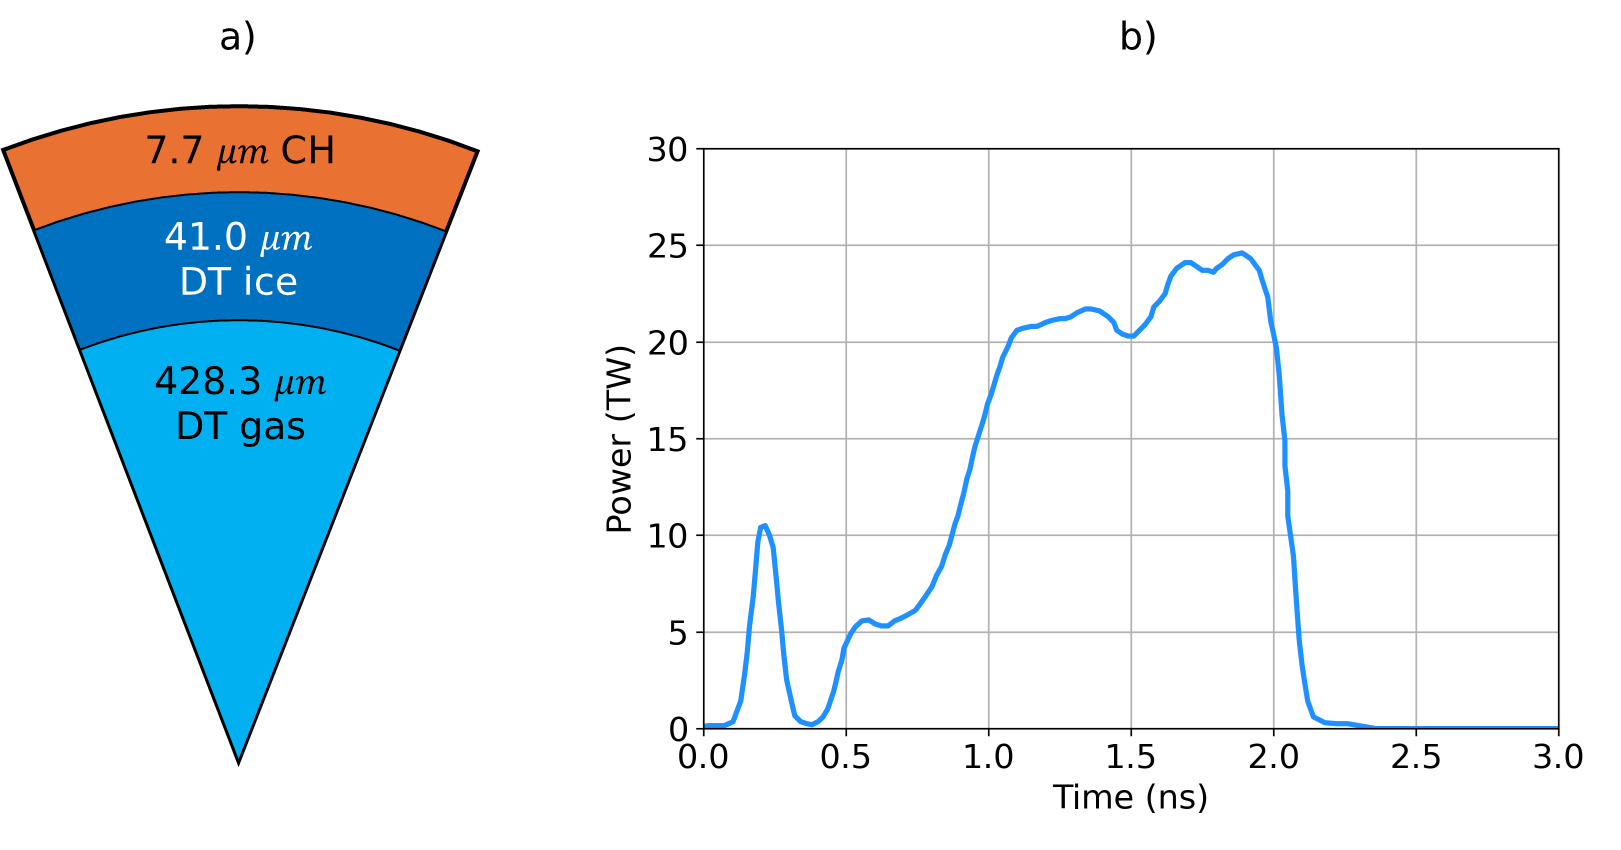
\includegraphics[width=0.9\linewidth]{Numerics/Images/89224_setup.png}
    \centering
    \caption{The initial conditions for \textsc{Omega} shot 89224.
    The shot was a cryogenic, DT implosion with materials and radii shown in panel a).
    Panel b) plots the incident laser pulse shape.}%
    \label{fig:89224_ICs}
\end{figure}

\begin{figure}[t!]
    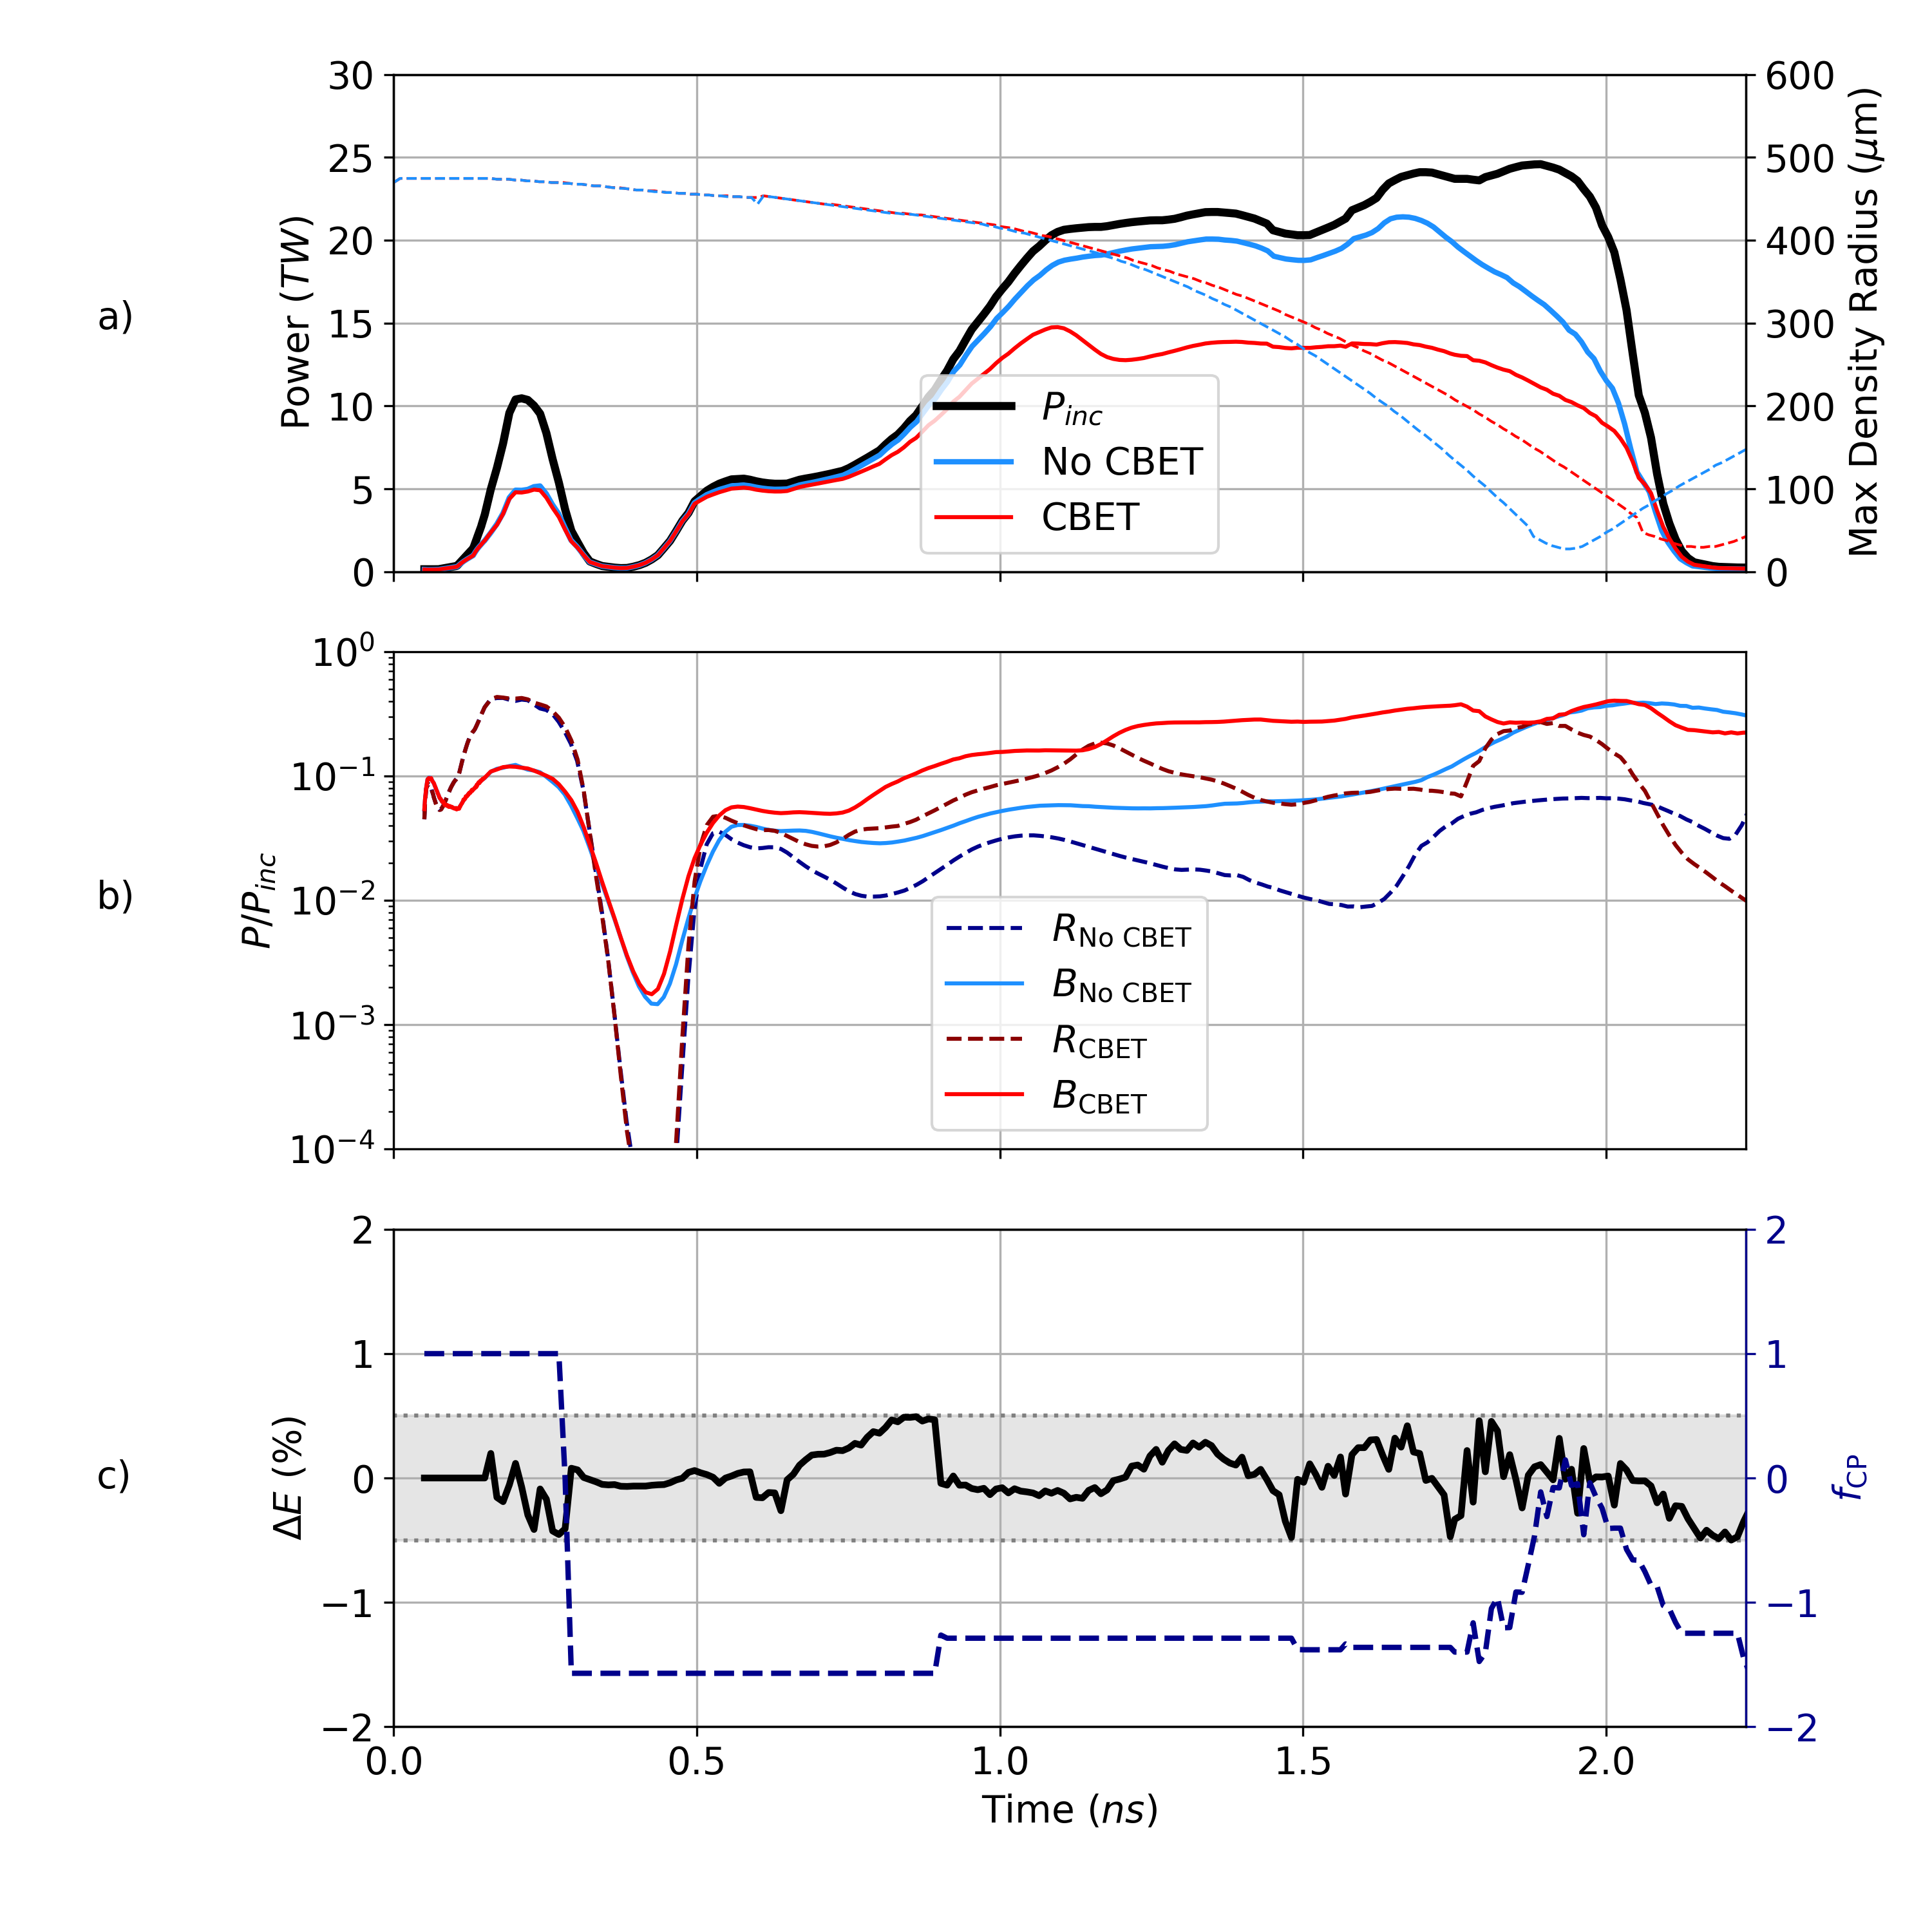
\includegraphics[width=0.9\linewidth]{Numerics/Images/89224_absorption.png}
    \centering
    \caption{\textsc{Chimera}-\textsc{Solas} simulation of \textsc{Omega} shot 89224.
    Panel a) shows the deposited power both from 2 separate simulations of 89224, one with and one without \ac{CBET} as red and blue solid curves respectively.
    The shell radius, defined at the radius of maximum density, is also plotted on the right axis as dashed curves.
    Panel b) plots the time resolved partition of non-absorbed light for these simulations.
    Plotted in c) is the energy conservation error after energy conservation was achieved, alongside the value of $f_{\text{CP}}$ that was used to achieve conservation.}%
    \label{fig:SOLAS_89224}
\end{figure}

\begin{table}[ht]
    \centering
    \caption{Integrated metrics from simulations of \textsc{Omega} 89224. \textsc{Lilac} metrics are from Refs.~\cite{patel_novel_2018,cao_interpreting_2019,crilly_neutron_2020}.}
    \begin{tabular}{cccccc} \hhline{=====}
    & $\text{Yield}$ & $\langle T_i \rangle$ & $t_{\text{bang}}$ & $V_{\text{imp}}$ \\ 
    & $\left(\times10^{14}\right)$ & $(\text{keV})$ & $(\text{ns})$ & $(\text{km/s})$ \\ 
    \hhline{-----}
    $\textsc{Lilac},\ \text{CBET}$ & 4.00 & 4.8 & 2.17 & 476  \\
    $\textsc{Chimera},\ \text{CBET}$ & 1.78 & 4.2 & 2.16 & 490  \\
    $\textsc{Chimera},\ \text{no CBET}$ & 6.77 & 6.2 & 1.94 & 661 \\ \hhline{======}
    \end{tabular}%
    \label{tab:SOLAS_89224_metrics}
\end{table}

A 1-D \textsc{Chimera}-\textsc{Solas} \ac{Rad-Hydro} simulation of \textsc{Omega} 89224 was performed to illustrate the effect that \ac{CBET} has on drive efficiency of direct-drive implosions.
Drive efficiency is lost primarily due a reduction in the magnitude of deposited energy.
A secondary effect is that the radii where deposition occurs is pushed slightly further away from the ablation surface.
This happens because beams only lose energy inside the \ac{CBET} resonance volume, which for backscatter \ac{CBET} occurs at the Mach-1 surface, as explained in Sec.~\ref{sec:Theory_sidescatter_backscatter_CBET}.
Therefore, the deposited power vs. radius curve is shifted to slightly higher radii.
Both of these effects are captured by a 3-D \ac{CBET} model coupled to 1-D \ac{Rad-Hydro}.

The initial conditions for shot 89224 are plotted in Fig.~\ref{fig:89224_ICs}.a, with vacuum outside the outer radius.
The incident laser pulse is also plotted in Fig.~\ref{fig:89224_ICs}.b, which has a total incident energy of $28.7\  \text{kJ}$.
An experimental yield of $1.17\times 10^{14}$ neutrons was observed for this shot.
A tabulated \texttt{Sesame} equation of state was used for each material \cite{mchardy_introduction_2018} and a $P_{1/3}$ radiation transport algorithm was used with tabulated opacities and emissivities from the \textsc{SpK} code~\cite{crilly_spk_2023}.
Thermal conduction was solved with using a fully implicit algorithm for flux-limited Spitzer conductivities~\cite{spitzer_transport_1953}.
The electron flux limiter was set by using the default \textsc{Chimera} direct-drive method,
\begin{equation}
    \label{eq:SOLAS_flime}
    f_{\text{lim},e} = 
    \begin{cases}
        0.06, & \text{if in picket pulse}\\
        0.15, & \text{otherwise}.
    \end{cases}
\end{equation}
The simulation domain was $r\in [0,1680]\ \mu\text{m}$, with a fixed radial resolution $\Delta_r = 1\ \mu\text{m}$.
Two simulations were conducted, one with the effect of \ac{CBET} on power deposition and one without.
In order to load balance the ray-trace and discretise \ac{CBET} interactions between different beams around the spherical $4\pi\ \text{sr}$, \textsc{Solas} used a sparse angular grid with $N_{\phi}=51$ and $N_{\theta}=30$ azimuthal and polar cells respectively.
At times earlier than $10\ \text{ps}$, a \textit{cold start} routine was employed, where $50\%$ of the incident power was deposited at the critical radius to create a finite scale length of underdense plasma, which rays could deposit and refract in.
Ray-traces were conducted every hydrodynamic timestep, without computing \ac{CBET} up to $150\ \text{ps}$\footnote{Note that the low intensity from this section of the pulse means that the \ac{CBET} gains are negligible.} after which a full ray-trace routine, including the effect of \ac{CBET} was conducted every $10\ \text{ps}$.
For hydrodynamic steps in between these \ac{CBET} ray-traces, the most recently computed $P_{\text{dep}}$ profile (normalised to 1 and then scaled to the incident power), was used as the laser source term for the timestep.
Parameter scans of the ray-trace frequency confirmed that the behaviour of \textsc{Omega} simulations is well converged with this frequency.

The spatially integrated absorbed power is plotted in Fig.~\ref{fig:SOLAS_89224}.a as solid curves.
$62.8\%$ and $83.9\%$ of the incident energy was absorbed for the \ac{CBET} and no-\ac{CBET} simulations respectively.
Also plotted as dashed curves are the shell trajectories from the two simulations.
It can be seen that the reduction is drive efficiency leads to a significantly slower implosion with a delayed bangtime.
Tab.~\ref{tab:SOLAS_89224_metrics} gives temporally and spatially integrated implosion metrics from the \textsc{Chimera}-\textsc{Solas} simulations, along with a comparison to a post-shot \textsc{Lilac} simulation which includes a 1-D model for \ac{CBET}.
Including \ac{CBET} in the \textsc{Chimera}-\textsc{Solas} simulation gives significantly better agreement across all metrics, which is primarily due to correctly capturing the reduction in absorption.
The most interesting metrics to compare across the codes when looking at the effect of \ac{CBET} in 1-D are the implosion velocity and bangtime, which are in excellent agreement with \textsc{Lilac}.
This is because these metrics are primarily functions of the absorbed laser energy, whereas the yield and burn averaged temperature additionally depend strongly on shock timing and compression~\cite{zhou_hydrodynamic_2007,trickey_physics_2024}.
Shock timing between codes is particularly sensitive to differences in the thermal conduction modelling, equation of states, grid resolution and preheat modelling, all of which are likely to have been different between the \textsc{Lilac} and \textsc{Chimera} simulations.
The strong agreement between the \textsc{Chimera} \ac{CBET} simulation and the \textsc{Lilac} results for the bangtime and implosion velocity metrics provide evidence that direct-drive implosions can be accurately modelled without using artificial multipliers to the laser power.

Fig.~\ref{fig:SOLAS_89224}.b plots the partition of the non-absorbed power for both simulations.
This is divided between \textit{blowby} light ($B$), which is light that left the computational domain travelling quasi parallel to the beam normal and \textit{reflected} light, which leaves the domain travelling quasi antiparallel.
Note that the plot is on a log axis.
Examining first the blue curves which are from the no-\ac{CBET} simulation, it can be seen that initially during the main pulse, from $t\sim 1.0\rightarrow1.6\ \text{ns}$, the reflected light fraction decreases while the blowby goes up.
This is because the critical radius converges, so the wings of the laser beam are less efficiently absorbed.
The reflected light fraction increases sharply at $t \sim 1.6\ \text{ns}$ and $t \sim 1.8\ \text{ns}$ for the no-\ac{CBET} and \ac{CBET} simulations respectively.
This corresponds to the time when the critical density crosses from the CH ablator material to DT fuel.
DT has a significantly lower ionisation state compared to the ablator and therefore the electron-ion collision frequency decreases, corresponding to a drop in the \ac{Inv-Brem} absorption and therefore an increase in the reflected light fraction.
Both simulations show that blowby light is the most significant loss of coupling both with and without \ac{CBET}, especially late in the implosion as the capsule converges.

Plotted in Fig.~\ref{fig:SOLAS_89224}.c are the laser energy conservation, $\Delta E$, and the modification to the caustic pump multiplier $f_{\text{CP}}$ that was found to achieve energy conservation.
The grey bounds indicate the accepted criteria to satisfy energy conservation, which was $0.5\%$ of the incident power.
The plot of $f_{\text{CP}}$ illustrates that the value remained constant over many timesteps and therefore only a single set of pump depletion iterations was required for the majority of timesteps.
This is not true late in the implosion, when the critical radius converges and \ac{CBET} is responsible for $\sim40\%$ reductions in deposited power.
At these times, caustic \ac{CBET} interactions are important and therefore $\Delta E$ is sensitive to the value of $f_{\text{CP}}$.
As shown in Sec.~\ref{sec:SOLAS_16beam_CBET} however, the iterations are believed to improve the fidelity of the modelling which is validated here by strong agreement with tuned, post-shot \textsc{Lilac} simulations.

\begin{figure}[t!]
    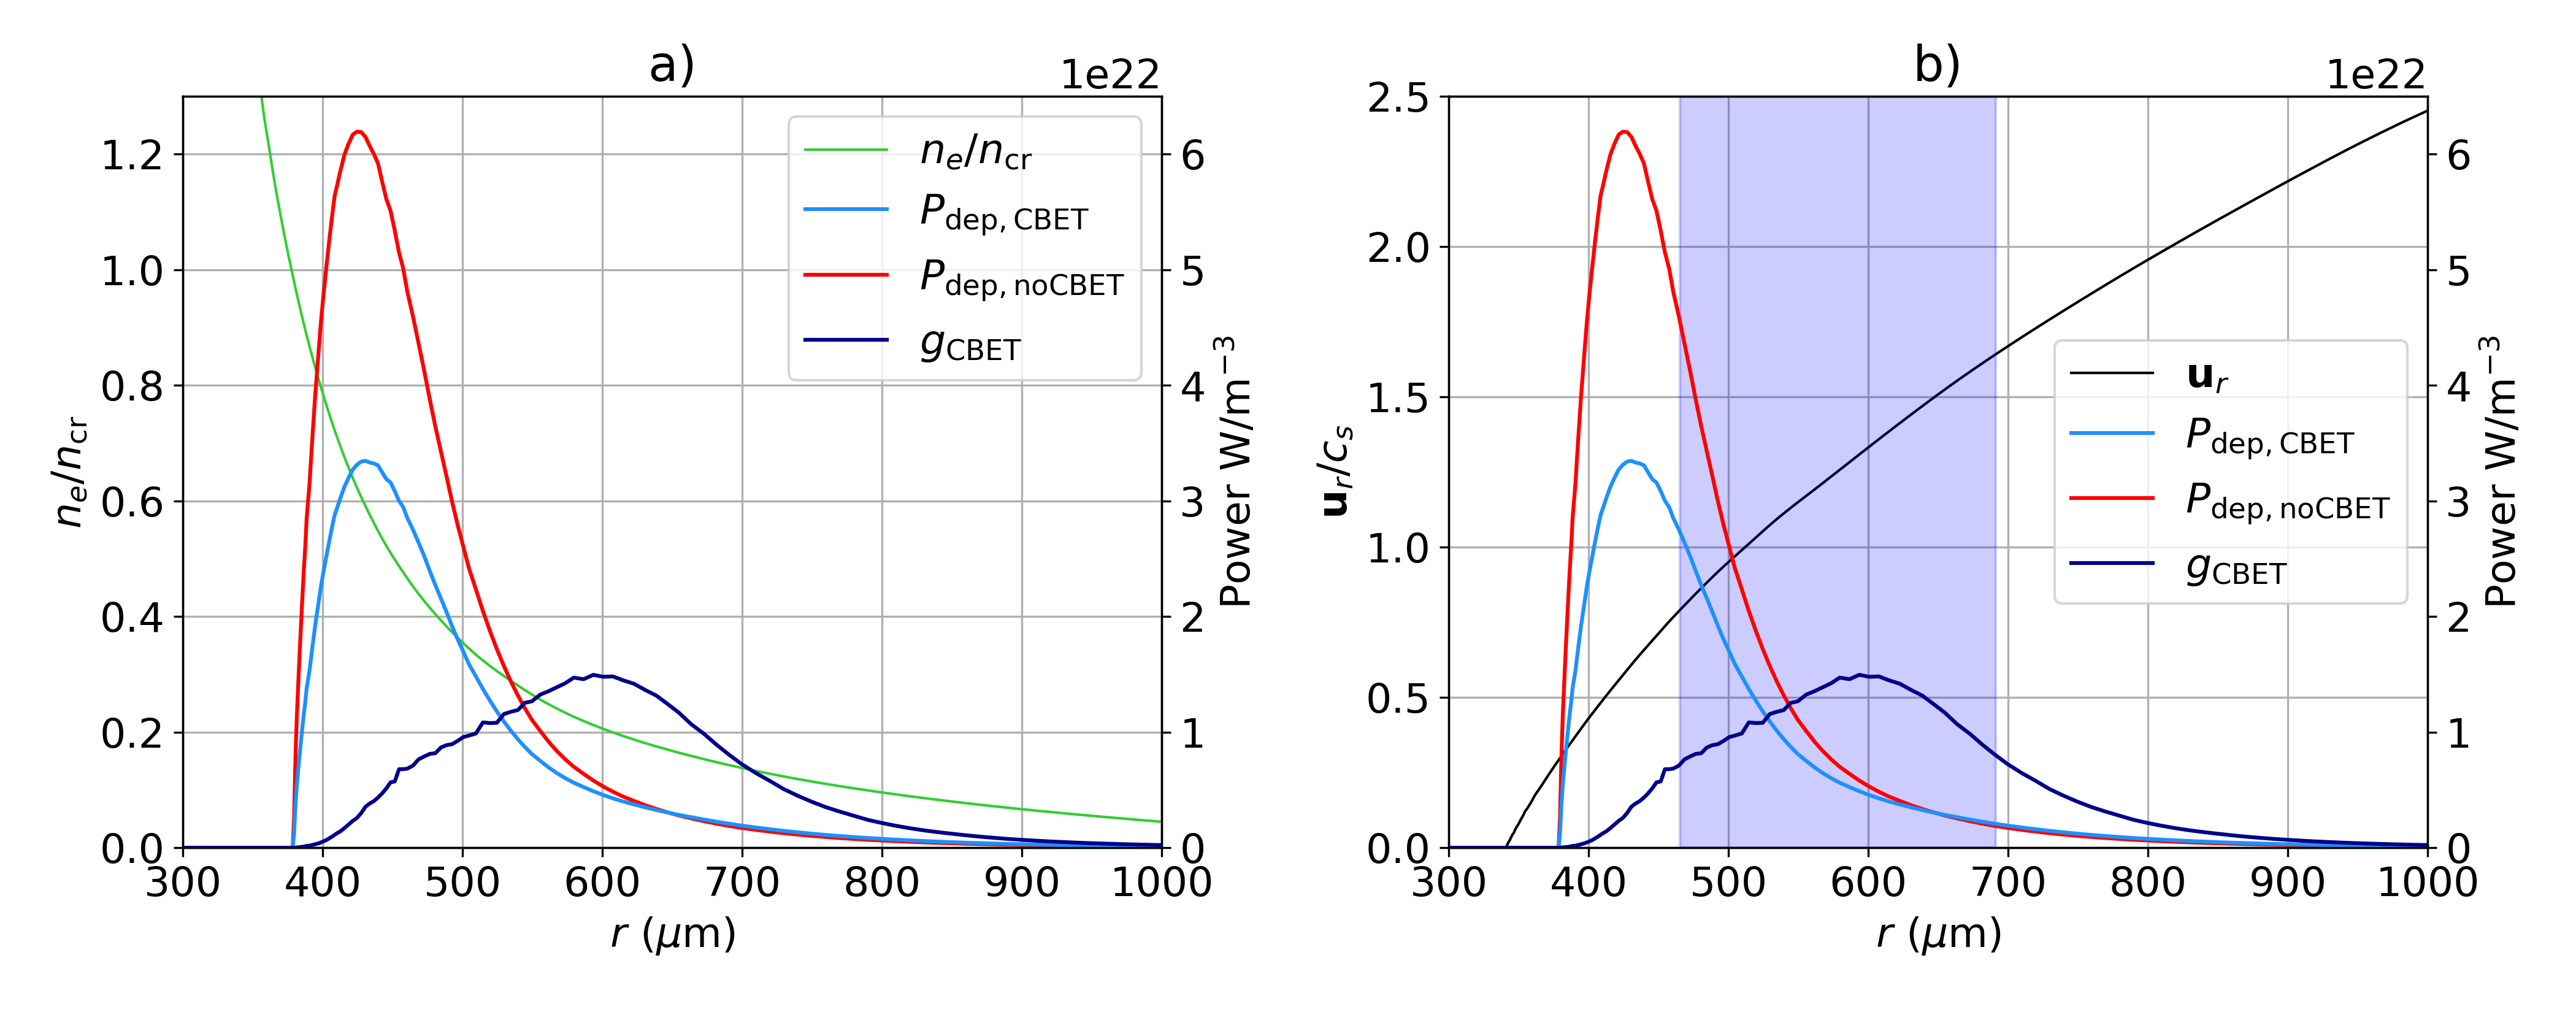
\includegraphics[width=\linewidth]{Numerics/Images/89224_it160_pdepcbet.png}
    \centering
    \caption{\ac{CBET} deposition diagnostics from $t=1.6\ \text{ns}$ into the \textsc{Chimera}-\textsc{Solas} simulation of \textsc{Omega} 89224, with \ac{CBET}.
    Both sub-plots plot the power deposition with and without \ac{CBET}, along with the $g_{\text{CBET}}$, which is defined as the sum of the absolute value of all power lost or gained by rays via \ac{CBET} in the cell.
    The electron density normalised to critical density and radial velocity normalised to the sound speed are also plotted in panel a) and b) respectively.
    The blue shaded region in b) represents the full-width half-maximum of the $g_{\text{CBET}}$ curve.}%
    \label{fig:SOLAS_89224_pdep}
\end{figure}

Plotted in Fig.~\ref{fig:SOLAS_89224_pdep}.a are the instantaneous power deposition profiles from the \textsc{Chimera}-\textsc{Solas} simulation with \ac{CBET} at $t=1.6\ \text{ns}$, alongside the $n_e$ profile in the under-dense region.
Note that the no-\ac{CBET} profile plotted here is not from the no-\ac{CBET} simulation of \textsc{Omega} 89224, but the power deposition from the field reconstruction ray-trace of the \ac{CBET} simulation, \textit{i.e.}, the deposition through the same hydrodynamic profiles, but without the effect of \ac{CBET} on the power deposition.
At this time, \textsc{Solas} estimates that \ac{CBET} reduces the deposition versus by about 40\% compared to the no-\ac{CBET} deposition.
No rays go beyond $n_{\text{cr}}$ and therefore all deposition occurs outside of the critical radius.
Also plotted in dark blue is the \ac{CBET} scattering, $g_{\text{CBET}}$, defined as the sum of the absolute value of all power lost or gained by rays due to \ac{CBET} in a \textsc{Solas} cell,
\begin{equation}
    \label{sec:SOLAS_cbet_scattering}
    g_{\text{CBET}}(\vec{x}) = \sum_{i}^{\text{rays}} \left| \Delta P_{i,\text{CBET}}(\vec{x}) \right|,
\end{equation}
where $\vec{x}$ represents the position of the power gain/ loss, discretised within cells on the \textsc{Solas} grid.
The deposition is broadly reduced only inside the peak of the scattering curve, because backscatter \ac{CBET} transfers energy from inbound light to outbound light in direct-drive.
Deposition is marginally increased outside the peak of the scattering curve, because the reflected and blowby light has been amplified due to \ac{CBET}.

These power profiles are also plotted alongside the coronal radial velocity profile, normalised to the sound speed.
The full-width half-maximum of the scattering curve is shown as the shaded blue region.
Resonance occurs close to the Mach-1 surface as expected, which is where the plasma flow shifts the frequencies of radially inbound and outbound light such that they can excite an \ac{IAW}.
%Note however, that the calculation of $c_s$ uses average ionisation and the simulation which computed $P_{\text{dep,CBET}}$ used the kinetic \ac{CBET} gain formulation, which can separately excite the fast and slow modes of the \ac{IAW}.
The peak scattering also is shifted slightly further out, because the outbound light mostly does not travel radially outward.
Assuming the fluid \ac{CBET} gain formulation and neglecting the $(\omega_j-\omega_i)$ in Eq.~\ref{eq:SOLAS_CBET_fluid_gain}, it can be shown that non-radial light shifts the resonance to larger $u_r$ and therefore greater radii.

%##################################################
\subsection{3-D Post Process of Absorption Non-Uniformity}%
\label{sec:SOLAS_IFRIIT_test}

\begin{figure}[t!]
    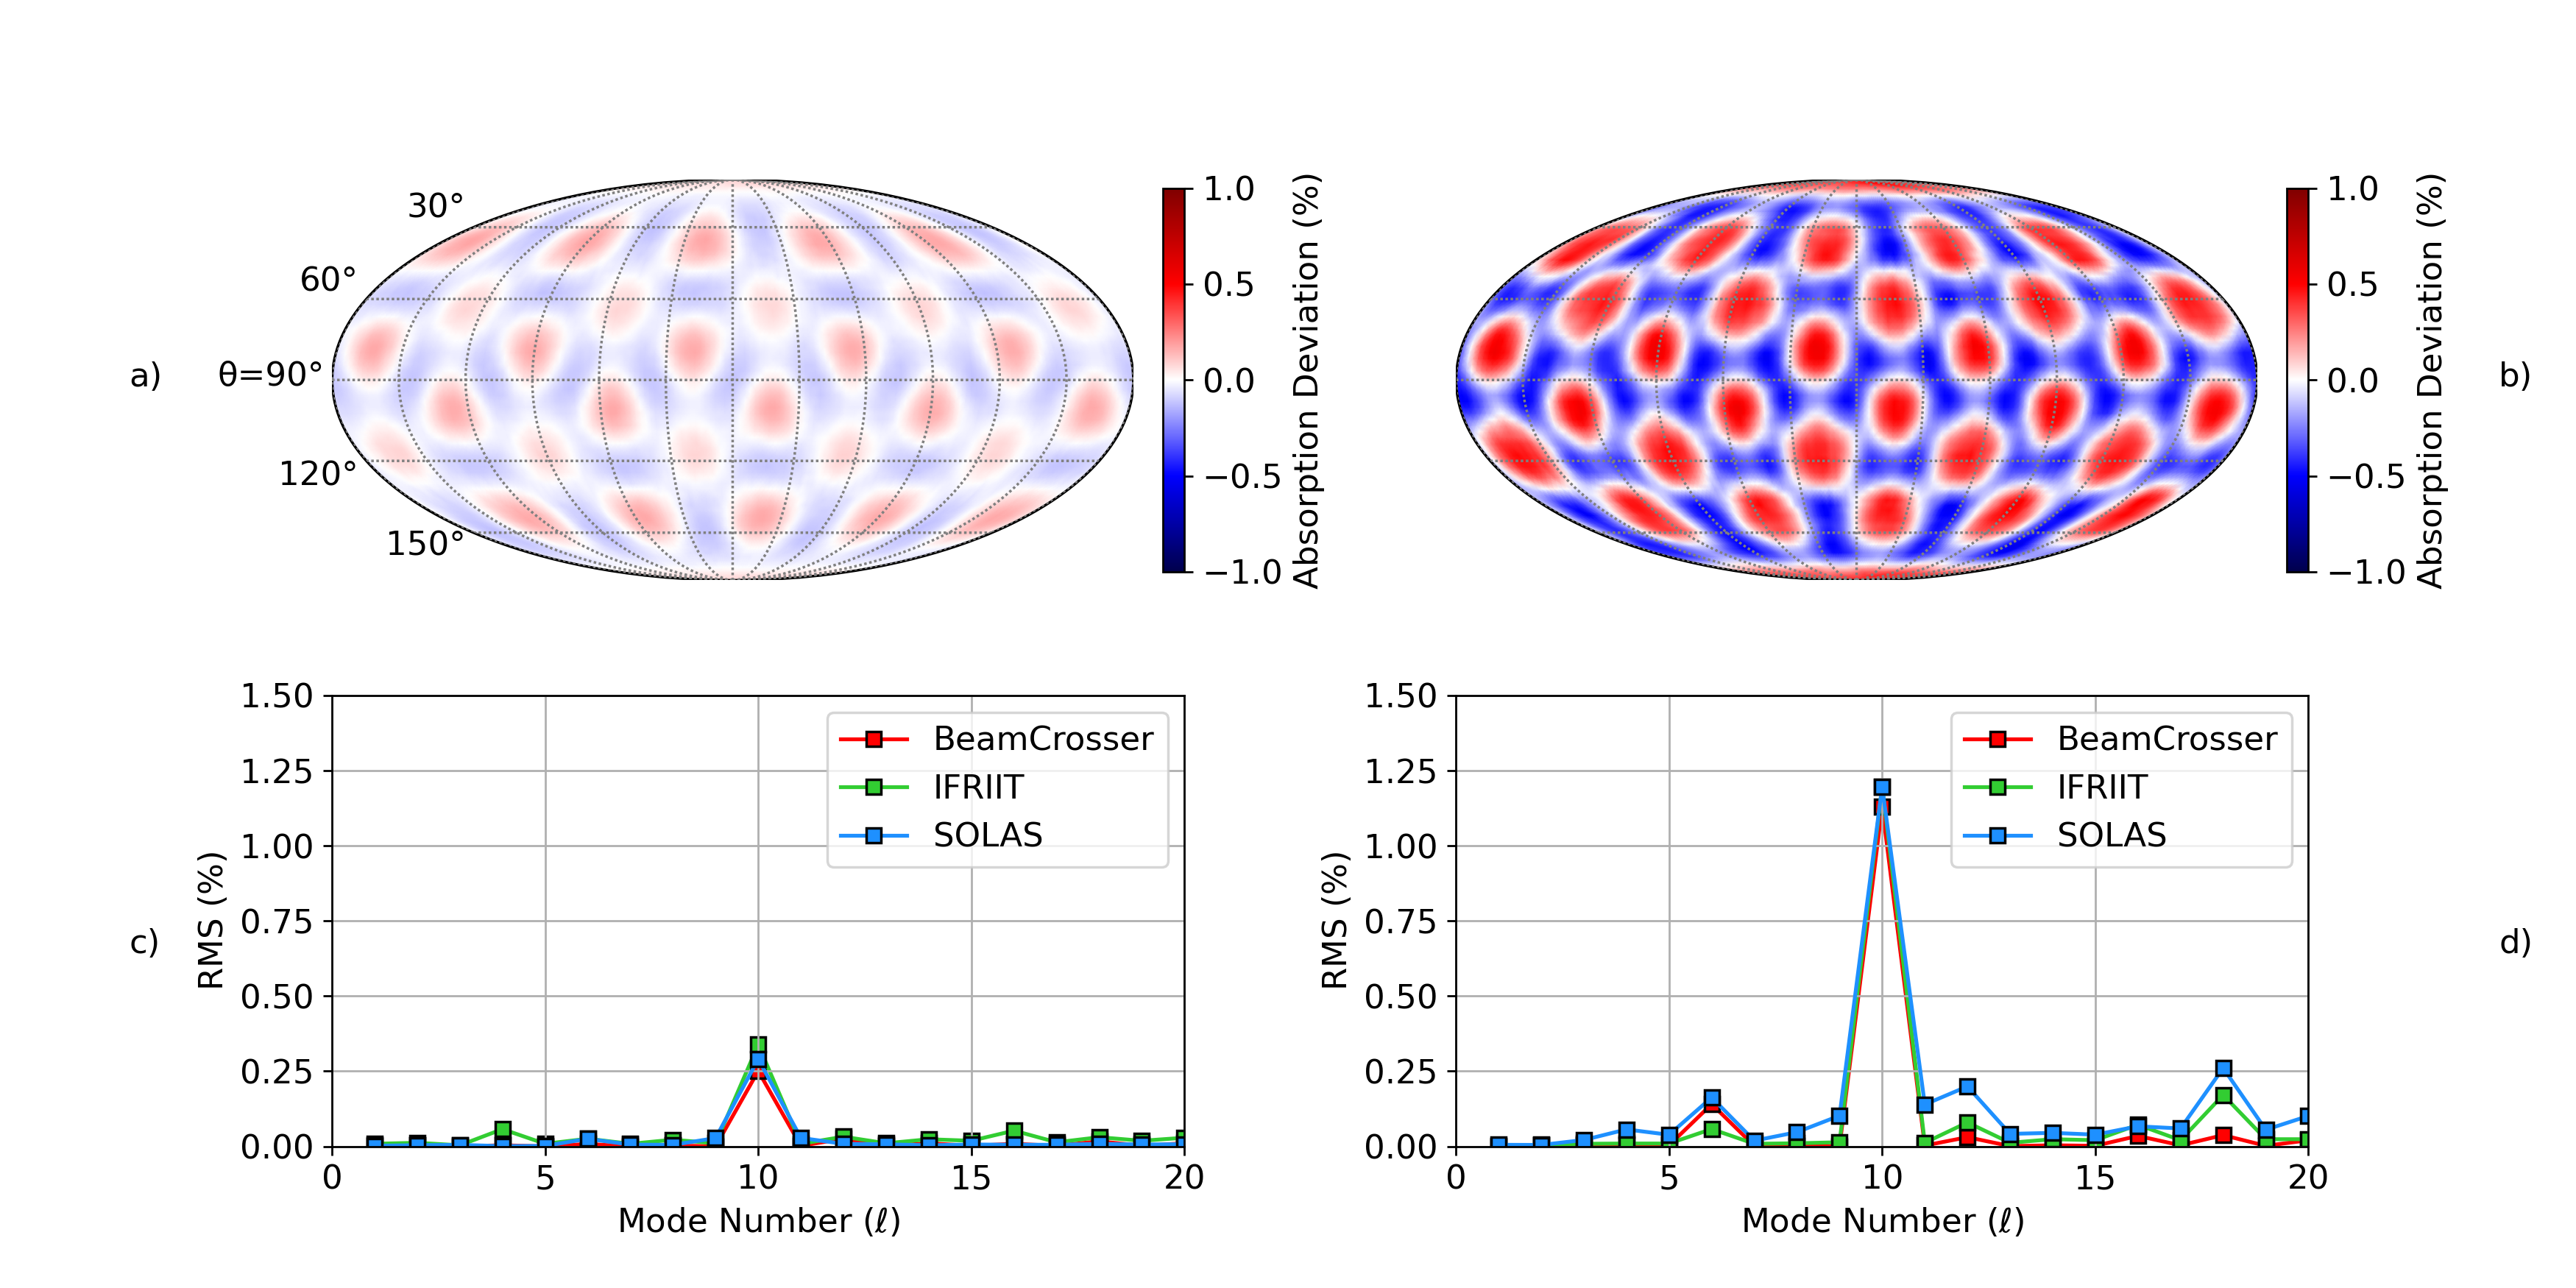
\includegraphics[width=1.0\linewidth]{Numerics/Images/DepositionAsymmetries_mollweide_xy32.png}
    \centering
    \caption{3-D \textsc{Solas} post-process of spherically symmetric hydrodynamic data obtained from a \textsc{Lilac} simulation of an \textsc{Omega} direct-drive implosion.
    Figures a) and b) show the deviation in radially integrated deposited power without and with \ac{CBET} respectively.
    Figures c) and d) plot the spherical harmonic modal decomposition for these maps alongside results from the \textsc{Ifriit} and \textsc{BeamCrosser} codes without and with \ac{CBET} respectively.}%
    \label{fig:SOLAS_qpR_IFRIIT_test}
\end{figure}

A final problem used to validate the \ac{CBET} model from \textsc{Solas} was to compute the instantaneous 3-D effect of \ac{CBET} on power deposition through spherically symmetric hydrodynamic data from a \textsc{Lilac} simulation of an \textsc{Omega} implosion.
The same problem has been computed with both the \textsc{Ifriit} and \textsc{BeamCrosser} codes allowing cross-code validation of the 3-D deposition asymmetry.
The \textsc{Lilac} profiles were taken from Ref.~\cite{colaitis_inverse_2021}, and the \textsc{Ifriit} and \textsc{BeamCrosser} results are presented in Ref.~\cite{colaitis_3d_2023}.
\ac{CBET} is known to enhance the beam-mode asymmetry which arises from the number and geometry of laser beams used to illuminate the target~\cite{edgell_mitigation_2017}.
Correctly capturing this enhancement of asymmetry relies on a field reconstruction algorithm with good treatment of laser caustics and sufficient ray statistics in every cell across the computational grid to reconstruct the field everywhere that \ac{CBET} is important.

This problem is a particularly stringent test of the grid discretisation for field reconstruction.
The use of an underlying spherical polar grid for the \textsc{Solas} semi-structured mesh leads to cells that vary in volume from pole to pole.
Some differences in the reconstructed field are therefore inevitable between the capsule waist and pole purely from this grid discretisation.
If this difference was insufficiently small, the power deposition with \ac{CBET} would contain a conspicuous mode-2 which, for simulations integrated with the hydrodynamics, would lead to undesirable stagnation asymmetries, purely seeded from the computational mesh.

The simulation had a radial domain $r\in[350,1362]\ \mu\text{m}$ with underlying grid resolution $\Delta_r=1\ \mu\text{m}$\footnote{Note that the adaptive radial resolution of the \textsc{Solas} mesh had a maximum radial resolution $\Delta_{r,\text{max}}=10\ \mu\text{m}$.}.
The full $4\pi\ \text{sr}$ was simulated, where an underlying polar mesh was used for the \textsc{Solas} grid with $N_{\phi}=160$ and $N_{\theta}=82$, which was then combined to give approximately equal area cells as described in Sec.~\ref{sec:SOLAS_mesh}.
Fig.~\ref{fig:SOLAS_qpR_IFRIIT_test}.a and Fig.~\ref{fig:SOLAS_qpR_IFRIIT_test}.b show the deviation in radially integrated power deposition from the mean value for the no-\ac{CBET} and \ac{CBET} simulations respectively.
The mode-10 pattern is clearly visible in both plots, although the magnitude is greatly increased by \ac{CBET}, as expected.
No clear mode-2 from the capsule pole to waist is seen which indicates that the \textsc{Solas} mesh is sufficiently close to equal-area to not result in significant grid artefacts.

A function, $f$ discretised over azimuthal ($\phi$) and polar ($\theta$) angles can be decomposed into spherical harmonics,
\begin{equation}
    f(\phi,\theta) = \sum_{\ell=0}^{\ell_{\text{max}}} \sum_{m=-\ell}^{m=\ell} a_{\ell m} Y_{\ell}^{m}(\phi,\theta),
\end{equation}
where $Y_{\ell m}$ are the spherical harmonic basis vectors and $a_{\ell m}$ are the associated coefficients \cite{colaitis_3d_2023}.
The modal asymmetry of a given mode number, $\ell$, is then defined as,
\begin{equation}
    \sigma_{\ell} = \sqrt{ \frac{1}{4\pi} \sum_{m=-\ell}^{m=\ell} a_{\ell m} a^*_{\ell m} },
\end{equation}
where the $a^*_{\ell m}$ is the conjugate of $a_{\ell m}$.
Fig.~\ref{fig:SOLAS_qpR_IFRIIT_test}.c plots the modal decomposition of the no-\ac{CBET} radially integrated power deposition deviation from the mean, \textit{i.e.} $\sigma_{\ell}$ up to mode $\ell=20$.
Excellent agreement is observed between \textsc{Solas} and the other codes.
The dominant mode is $\ell=10$, as is expected due to the beam port geometry.

Fig.~\ref{fig:SOLAS_qpR_IFRIIT_test}.d plots the same, but now for the power deposition including \ac{CBET}.
As is also seen in the skymaps, the asymmetry is significantly amplified by \ac{CBET}.
Good agreement is again observed between \textsc{Solas}, \textsc{Ifriit} and \textsc{BeamCrosser} across the spectrum.
\ac{CBET} appears to induce small amplitude modes other than just the $\ell=10$ such as $\ell=6$, $\ell=12$ and $\ell=18$.
These are all multiples of 6, and therefore are likely induced by some \textsc{Omega} beam ports having 6 nearest neighbours~\cite{boehly_upgrade_1995,simon_lle_1989}.
Small differences are observed between all codes, which is expected due to the different solvers and grids employed by each.
\textsc{Solas} appears to slightly overestimate the modes 9 and 11, which have negligible values for both \textsc{Ifriit} and \textsc{BeamCrosser}.
This is potentially due to the ray shape function smearing routine used, that was described in Sec.~\ref{sec:SOLAS_ray_propagation}, which smear power from a ray in one cell into neighbours.
This could bleed some $\ell=10$ into neighbouring modes.
In future, a more robust spherical harmonic smoothing could be introduced to address this issue, although the effect is not likely to be significant for integrated simulations due to the small amplitude.

\begin{figure}[t!]
    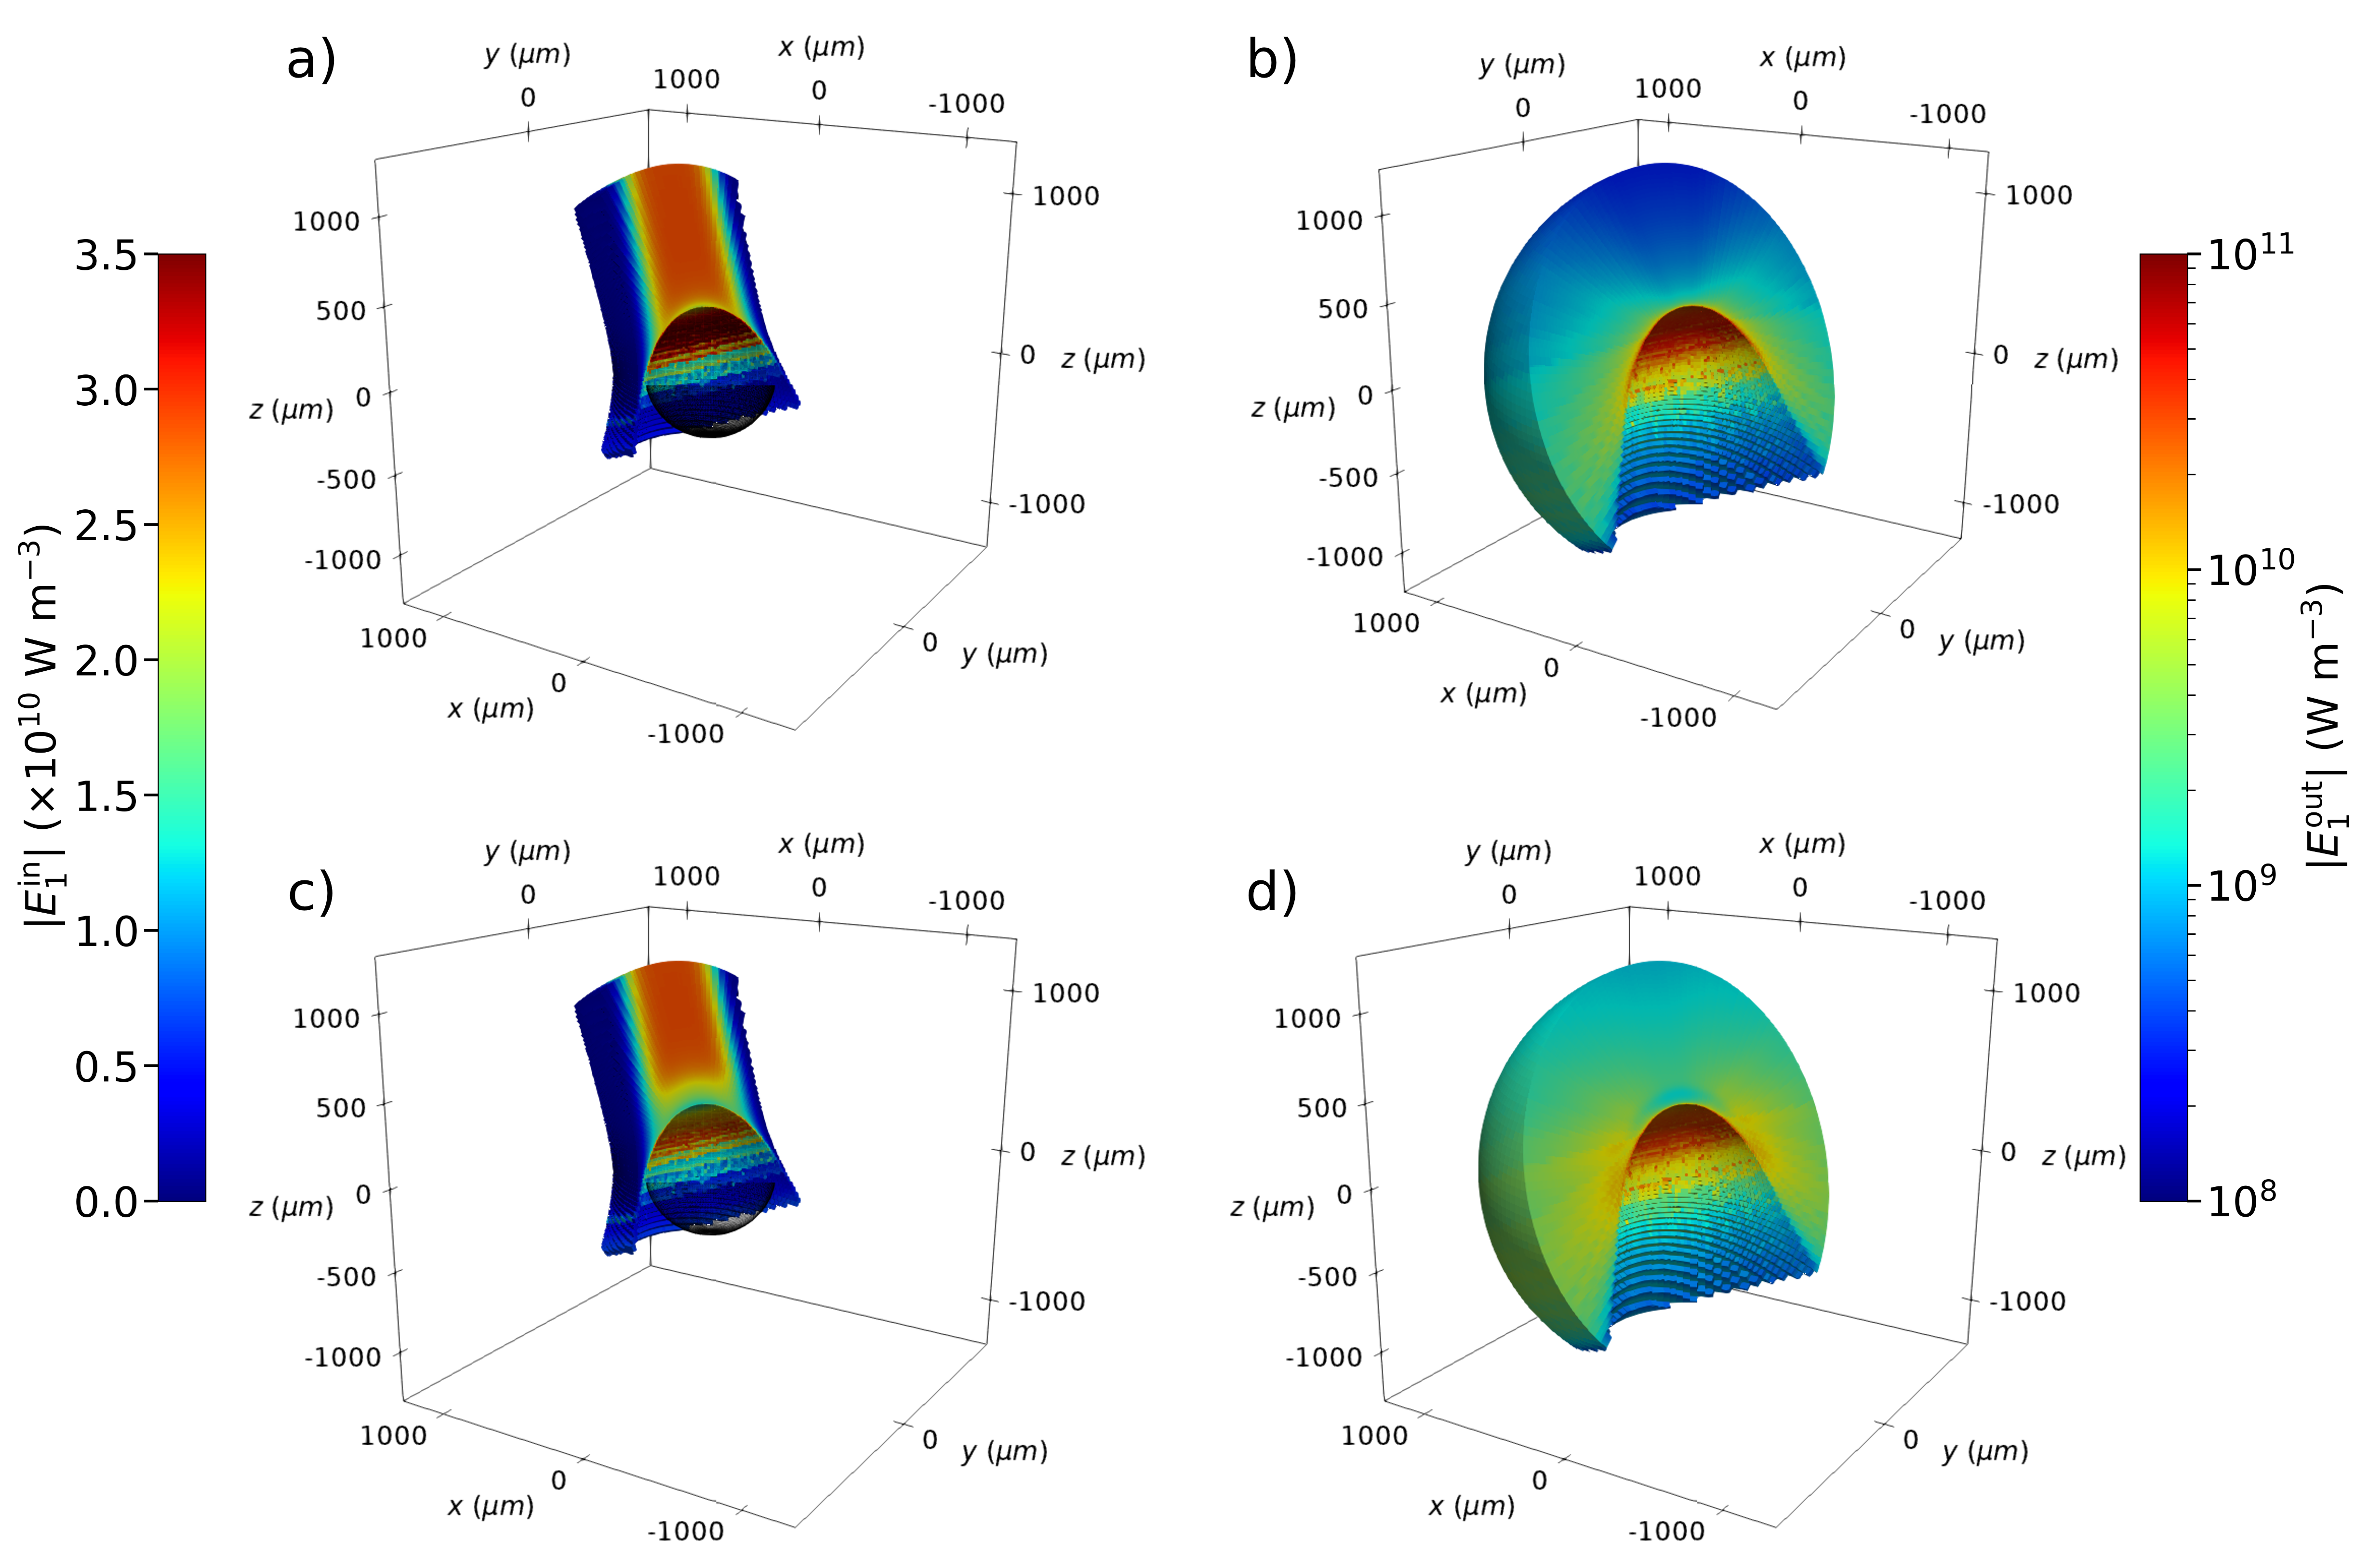
\includegraphics[width=1.0\linewidth]{Numerics/Images/IFRIIT_test_fields.png}
    \centering
    \caption{Electric fields from the 3-D post-process.
    Panels a), b), c) and d) plot the incident sheet without \ac{CBET}, the reflected sheet without \ac{CBET}, the incident sheet with \ac{CBET} and the reflected sheet with \ac{CBET} respectively.
    The critical surface is plotted with the inbound sheets as a transparent spherical wireframe.
    Note that the outbound sheets are plotted on a log scale.}%
    \label{fig:SOLAS_IFRIIT_test_fields}
\end{figure}

The incident and reflected sheet fields\footnote{Note that incident and reflected here refer to which sheet the ray belongs to, \textit{i.e.} if it is before or after the caustic location.} for a single beam both with and without \ac{CBET} are plotted in Fig.~\ref{fig:SOLAS_IFRIIT_test_fields}.
The incident fields without and with \ac{CBET} are plotted in Fig.~\ref{fig:SOLAS_IFRIIT_test_fields}.a and Fig.~\ref{fig:SOLAS_IFRIIT_test_fields}.c respectively, and share the left colourbar.
The inbound \ac{CBET} sheet field shows a clear depletion of the field strength near the critical surface compared to the no-\ac{CBET} field, which is the result of energy transfer from radially inward propagating light to outward travelling light via backscatter.
This leads to the reduction in absorbed energy.
Fig.~\ref{fig:SOLAS_IFRIIT_test_fields}.b and Fig.~\ref{fig:SOLAS_IFRIIT_test_fields}.d plot the reflected fields without and with \ac{CBET} respectively, and share the right colourbar.
The reflected sheet travels mostly radially outward and therefore has been significantly amplified by the \ac{CBET} backscatter mechanism compared to the no-\ac{CBET} case.
In the absence of \ac{CBET}, the field strength of the reflected sheet is significantly lower than the incident sheet field strengths for two reasons.
Firstly, peak absorption occurs at the maximum radial penetration depth of the light into plasma, which is typically close to where rays experience their caustic and change sheet.
Additionally, the rays diverge after reflecting from the critical surface leading to a reduction in ray amplitude and therefore field strength.


\iffalse

%###############################################################################################################################
%###############################################################################################################################
%###############################################################################################################################
\section{Future Model Extensions}

Say that there is even more laser/ CBET physics that is interesting and can be implemented within the ray-tracing framework.
Some are straightforward to implement, while others more difficult and computationally expensive.

%################################################################################
%################################################################################
\subsection{Langdon Effect on Absorption}

Describe Langdon from a kinetic perspective and why it reduces absorption.
Describe how you can fit it and include as a modification to ray-tracing absorption if you have the field/ intensity.
Describe the magnitude of the effect for ICF like conditions.
Describe breifly how it would be implemented, say it would not be difficult.

%################################################################################
%################################################################################
\subsection{Langdon Effect on CBET}

Describe what this is.
Say that it is important for high overlapping intensities, eg hohlraum LEH.
Say that it is thought to stabilise the CBET interaction in indirect drive configurations and remove the need for artificial clamps.
Describe briefly how it would be implemented, say it would not be difficult.

%################################################################################
%################################################################################
\subsection{Polarised CBET}

Describe how ion acoustic waves are driven by beat between electric fields from light and therefore is polarisation dependent.
Say how on \textsc{Omega}, RPP smoothing means that each beam is split into 2 sub-beams with linear polarisation.
Say that these do not have a symmetry to the configuration about the sphere.
Say that this leads to mode-1 on \textsc{Omega}.
Say that you can track polarisation of rays and trace these sub-beams independently.
Would make it more expensive, but definitely feasible.

%################################################################################
%################################################################################
\subsection{Bandwidth for CBET Mitigation Studies}

Describe how bandwidth should reduce LPI growth rates.
Understanding the desired bandwidth to mitigate CBET is a key consideration for design of future laser systems.
Fields can be modified to include discrete wavelengths to model bandwidth.

%################################################################################
%################################################################################
\subsection{Additional LPIs}

Could look at TPD, SBS and SRS.
In theory not a difficult problem to do backscatter, but side-SRS is difficult, because additional rays would need to be launched.
This could make the model more useful to indirect-drive experiments and design of ignition scale direct-drive facilities, where SRS is thought to be important energetically due to long scale lengths.

\fi

%###############################################################################################################################
%###############################################################################################################################
%###############################################################################################################################
\section{Conclusions}

This chapter presented the implementation and validation of a 3-D ray-trace and \ac{CBET} model, \textsc{Solas}, for the 3-D \ac{Rad-Hydro} code \textsc{Chimera}.
Prior to this work, a simple 1-D ray-trace was used to model the laser for direct-drive implosions which was strongly detrimental to the ability of the code to accurately model these experiments.
Radially tracing rays inward, even for 1-D \ac{Rad-Hydro} simulations, misses the important interplay between the convergence of the target and loss of deposition.
The lack of a \ac{CBET} model, which is responsible for significant energy coupling loss at \textsc{Omega} laser facility energy scale implosions, also meant that deposited power had to be reduced in an \textit{ad-hoc} manner to obtain agreement with experiments.
These factors severely limited the predictive capability of the code to model these experiments.

Sec.~\ref{sec:SOLAS_raytrace} described the implementation of the 3-D ray-trace in the \textsc{Solas} laser package.
An adaptive solver is used to trace rays through a semi-structured Eulerian mesh in Cartesian, cylindrical or spherical geometries. 
Validation of this implementation was also presented.
The 3-D laser ray-trace enables \textsc{Chimera} to model direct-drive implosions and other laser-driven \ac{HEDP} experiments.
It is also a crucial prerequisite to a ray-based \ac{CBET} model.

Issues with ray-based \ac{CBET} models often stem from a poorly reconstructed laser electric field profile.
The approach taken in \textsc{Solas} to obtain the electric field was described in Sec.~\ref{sec:SOLAS_field_reconstruc}, which is to trace a set of neighbouring rays around each ray and then relate the area of the ray to the field strength.
Validation problems were conducted for this section which illustrated that this approach yields excellent agreement with the wave-based solver \textsc{Lpse}.
Caustics are also identified and the field near them is capped to a diffraction limited value.
Validation problems showed that the field solver was robust and suitable for use within the \ac{CBET} model.

The implementation of the \textsc{Solas} \ac{CBET} model was described in Sec.~\ref{sec:SOLAS_cbet_model}.
This model employs the linear kinetic or fluid gain formulations and the reconstructed field to estimate power changes of rays due to \ac{CBET}.
Fixed point iteration is then used to find the equilibrium solution and additional energy conservation iterations can be used to account for small errors in the caustic field reconstruction.
Validation problems against \textsc{Lpse} and the ray-based \textsc{BeamCrosser} post-processor demonstrated that \textsc{Solas} correctly computes \ac{CBET} for direct-drive conditions in Cartesian and cylindrical geometries.

A 1-D, spherical \ac{Rad-Hydro}, \textsc{Chimera}-\textsc{Solas} simulation of the \textsc{Omega} shot 89224 was presented in Sec.~\ref{sec:SOLAS_89224}, alongside a comparison to a \textsc{Lilac} simulation.
The \ac{CBET} model behaved as expected, significantly reducing the power deposition and slowing the implosion.
Excellent agreement was obtained between \textsc{Chimera}-\textsc{Solas} and \textsc{Lilac} for integrated parameters which primarily depend on the amount of energy coupled to the target.
Sec.~\ref{sec:SOLAS_IFRIIT_test} presented a 3-D post-process of spherically symmetric hydrodynamic data from a \textsc{Lilac} simulation.
The power deposition asymmetry was compared to the \textsc{Ifriit} and \textsc{BeamCrosser} codes and good agreement was found with those models.
\ac{CBET} was shown to significantly enhance the deposition asymmetries as expected.
The results from this section showed that the \textsc{Solas} \ac{CBET} model functions as expected in spherical geometry and therefore \textsc{Chimera}-\textsc{Solas} is capable of performing 3-D spherical direct-drive implosions with \ac{CBET} which could previously only be conducted with the \textsc{Aster}-\textsc{Ifriit} code combination.
